%%%%%%%%%%%%%%%%%%%% author.tex %%%%%%%%%%%%%%%%%%%%%%%%%%%%%%%%%%%
%
% sample root file for your "contribution" to a contributed volume
%
% Use this file as a template for your own input.
%
%%%%%%%%%%%%%%%% Springer %%%%%%%%%%%%%%%%%%%%%%%%%%%%%%%%%%%%%%%%%


% RECOMMENDED %%%%%%%%%%%%%%%%%%%%%%%%%%%%%%%%%%%%%%%%%%%%%%%%%%%
\documentclass[graybox]{svmult}

% choose options for [] as required from the list
% in the Reference Guide

\usepackage{mathptmx}       % selects Times Roman as basic font
\usepackage{helvet}         % selects Helvetica as sans-serif font
\usepackage{courier}        % selects Courier as typewriter font
\usepackage{type1cm}        % activate if the above 3 fonts are
                             % not available on your system

\usepackage{makeidx}         % allows index generation
\usepackage{graphicx}        % standard LaTeX graphics tool
                             % when including figure files
\usepackage{multicol}        % used for the two-column index
\usepackage[bottom]{footmisc}% places footnotes at page bottom

\usepackage{subcaption}
\captionsetup{compatibility=false}
\usepackage{multirow}

\usepackage[
binary-units=true,
per-mode=symbol,
detect-weight=true,
]{siunitx}

% figure path and their extensions so you won't have to specify these with
% every instance of \includegraphics
\graphicspath{{figures/}}
\DeclareGraphicsExtensions{.pdf,.jpg,.png}

\usepackage[
backend=biber,
%style=numeric, % Orders alphabetically by author last name
% style=ieee, % Orders by appearance in text
%citestyle=numeric-comp,
% citestyle=ieee,
%maxnames=6,
%minnames=1,
]{biblatex}

\bibliography{references}

\usepackage{booktabs}

\usepackage{refcheck}
\norefnames

% see the list of further useful packages
% in the Reference Guide

\makeindex             % used for the subject index
                       % please use the style svind.ist with
                       % your makeindex program

%%%%%%%%%%%%%%%%%%%%%%%%%%%%%%%%%%%%%%%%%%%%%%%%%%%%%%%%%%%%%%%%%%%%%%%%%%%%%%%%%%%%%%%%%

\begin{document}

\title{System Integration of RISC-V Processors with FD-SOI}
% Use \titlerunning{Short Title} for an abbreviated version of
% your contribution title if the original one is too long
\author{Ben Keller and Borivoje Nikoli\'{c}}
% Use \authorrunning{Short Title} for an abbreviated version of
% your contribution title if the original one is too long
\institute{Ben Keller \at NVIDIA Research, 2788 San Tomas Expressway, Santa Clara, CA 95051 \email{benk@nvidia.com}
\and Borivoje Nikoli\'{c} \at Department of Electrical Engineering and Computer Sciences, University of California, Berkeley, Berkeley, CA 94720 \email{bora@eecs.berkeley.edu}}
%
% Use the package "url.sty" to avoid
% problems with special characters
% used in your e-mail or web address
%
\maketitle

\abstract{TODO - abstract}


%-------------------------------------%
\section{SoC Design in FD-SOI}

FD-SOI technology presents unique opportunities for system integration to achieve resilient and energy-efficient operation of digital systems.
The use of the free, open RISC-V instruction set architecture (ISA) for processor design allows custom experimentation and tight integration of power management features.
By integrating voltage regulators, clock generators, resilient SRAMs, and body-bias generators into a single die, the system can respond rapidly to variation and implement closed-loop feedback algorithms for energy savings at high performance.
The Raven-3 and Raven-4 testchips were developed to explore these concepts and prove the practicality of efficient system integration in FD-SOI~\cite{Keller2017Dissertation}.

\subsection{Raven-3}

The Raven-3 testchip features energy-efficient integrated voltage regulation, adaptive clocking, resilient SRAMs, and a fully-featured application processor~\cite{Zimmer2016}.
A block diagram of the system is shown in Figure~\ref{fig:6-raven3-blockdiagram}.

\begin{figure}
  \centering
  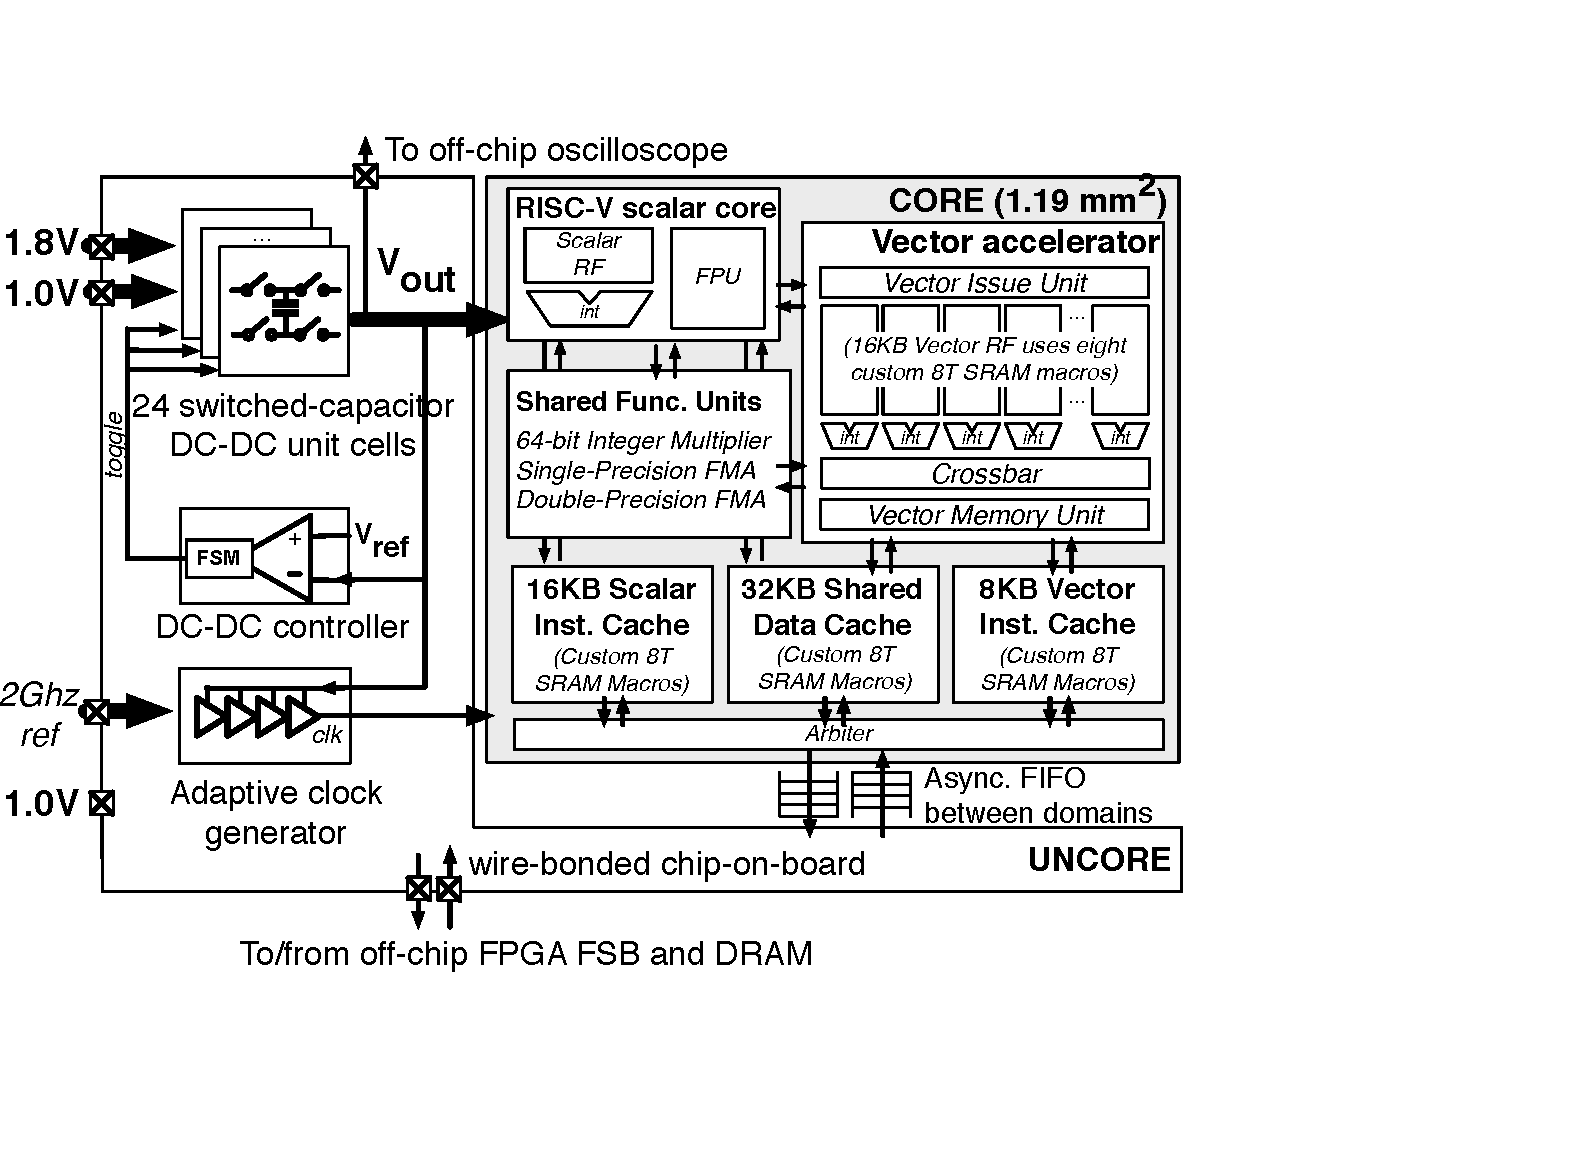
\includegraphics[width=0.9\textwidth]{6-raven3-blockdiagram}
  \caption{A block diagram of the Raven-3 testchip~\cite{Zimmer2016} ({\textcopyright} 2016 IEEE, reprinted with permission).}
  \label{fig:6-raven3-blockdiagram}
\end{figure}

The application core in Raven-3 is Rocket Chip, a 64-bit in-order energy-efficient processor.
The Hwacha vector accelerator can accelerate common computational kernels, achieving energy-efficient dataflow via its systolic operation and tight coupling with the Rocket core.
The SRAMs in Rocket's instruction and data caches, as well as the Hwacha register file, are implemented as custom-designed, highly resilient macros that can operate at low voltages.
Together, these components comprise the core digital logic of the system.

The core voltage is supplied by an integrated switched-capacitor (SC) DC-DC converter.
\SI{1.0}{\volt} and \SI{1.8}{\volt} supplies are downconverted to rippling output voltages averaging \SI{0.9}{\volt}, \SI{0.67}{\volt}, and \SI{0.5}{\volt} depending on the reconfigurable converter topology.
The \SI{1.0}{\volt} supply can also be passed directly to the core in a bypass mode.
The converter is subdivided into twenty-four \SI{90}{\micro\meter} $\times$ \SI{90}{\micro\meter} unit cells that are located near the core voltage area.

The core clock is generated by an adaptive clock generator that selects clock edges from a 16-phase DLL output as determined by the delay through a replica critical path supplied by the core voltage.
The replica path is made up only of inverters, with the depth of the path programmable via selectable muxes.
The generated clock is supplied to all register and SRAM sinks in the core voltage domain.

The IP blocks and their control registers, IO cells, and HTIF logic comprise the uncore voltage domain, which operates at a fixed \SI{1}{\volt} and fixed frequency.
Because the uncore and core may be asynchronous depending on the operating mode, bisynchrounous FIFOs guard all communication between them as shown in Figure~\ref{fig:5-bisync-fifo}.
Level shifters are inserted on signals crossing the domains to ensure correct operation as the core voltage varies.

\begin{figure}
  \centering
  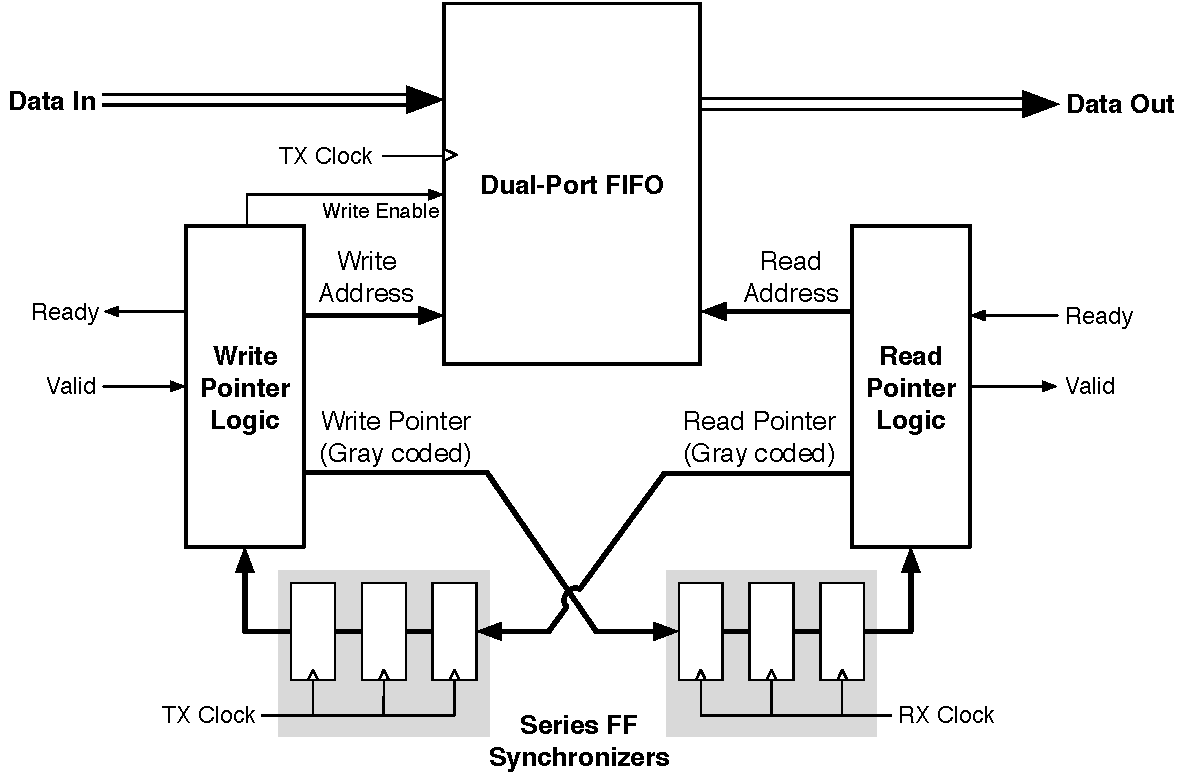
\includegraphics[width=\textwidth]{5-bisync-fifo}
  \caption{The standard bisynchronous FIFO.}
  \label{fig:5-bisync-fifo}
\end{figure}

\begin{figure}
  \centering
  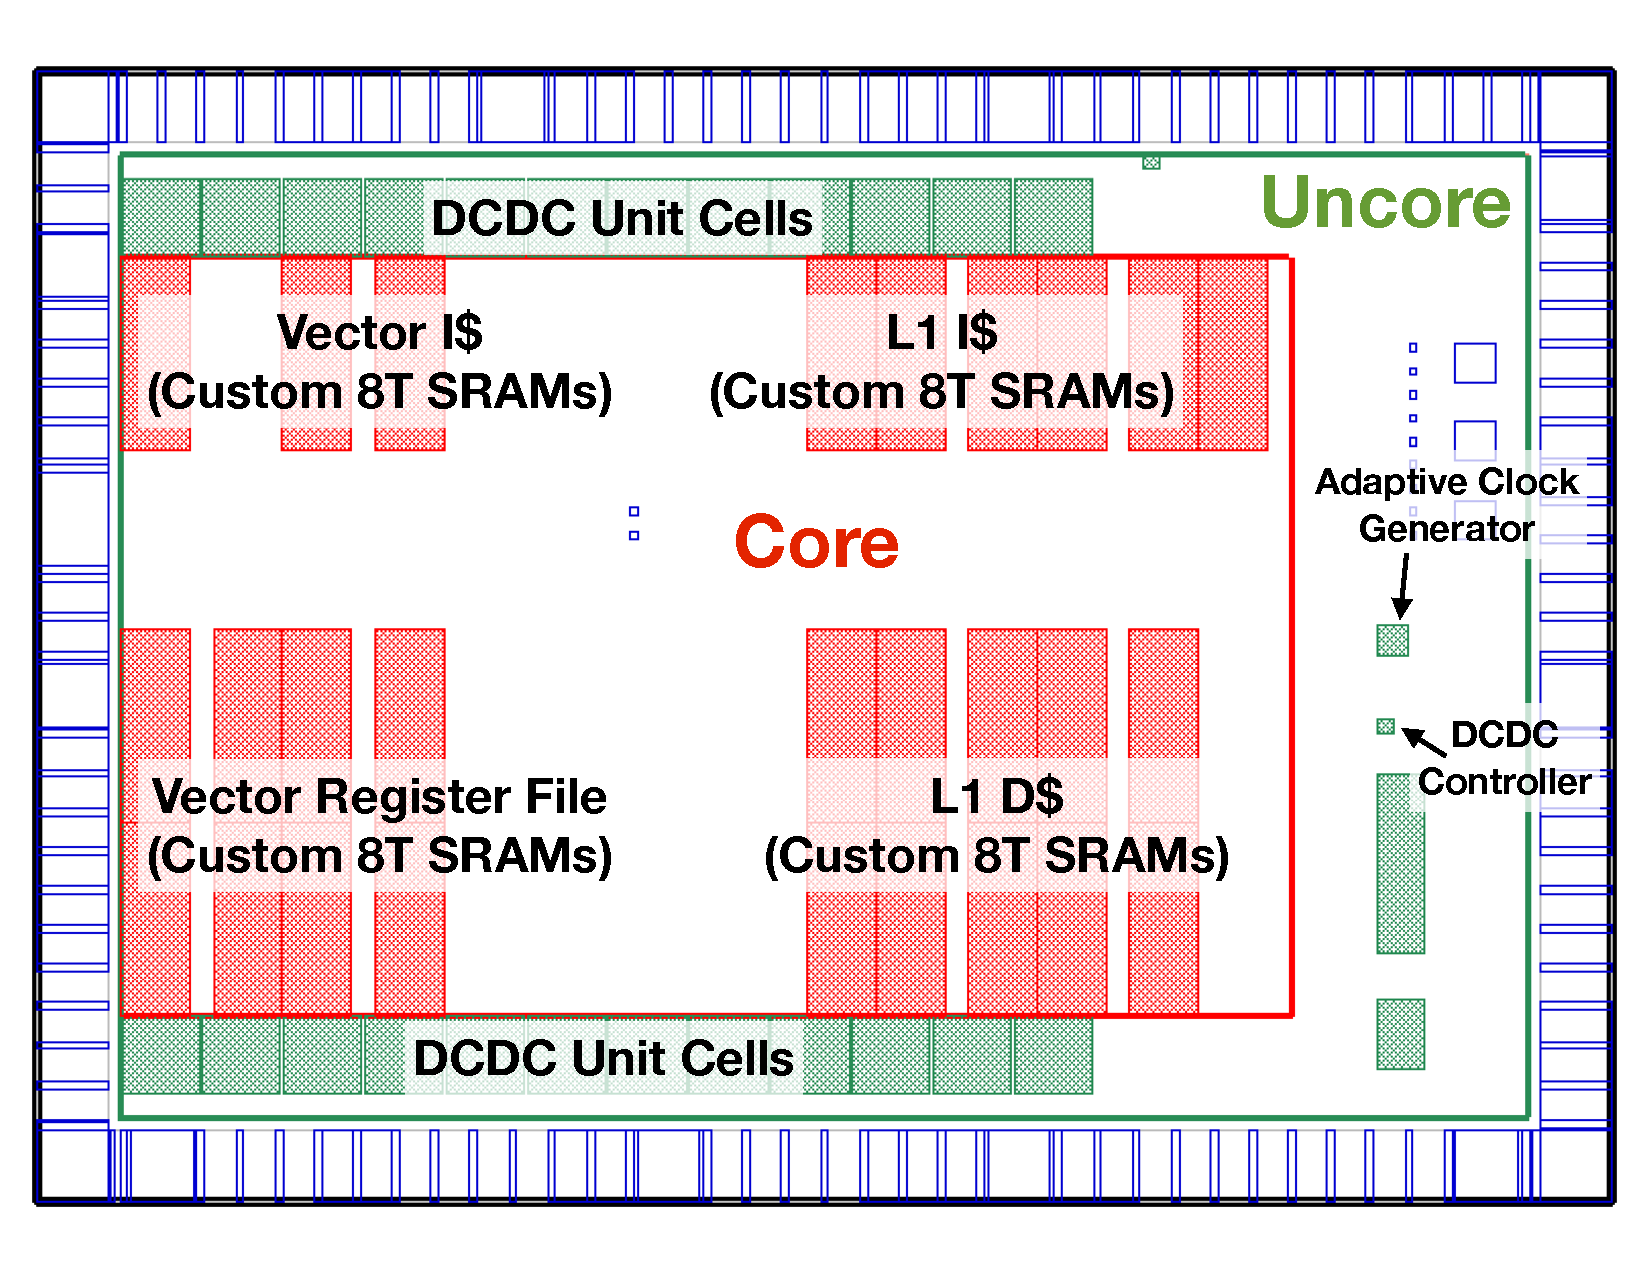
\includegraphics[width=0.6\textwidth]{6-raven3-floorplan}
  \caption{Annotated floorplan of the Raven-3 testchip~\cite{Zimmer2016} ({\textcopyright} 2016 IEEE, reprinted with permission).}
  \label{fig:6-raven3-floorplan}
\end{figure}

A multivoltage and multiclock design flow was used to construct the processor.
Figure~\ref{fig:6-raven3-floorplan} shows the processor floorplan, with the larger core voltage domain in red separated from the smaller uncore voltage domain to the right of the chip.
The custom SRAMs were manually placed within the core voltage domain.
The SS-SC unit cells surround the core to minimize voltage drop.
Two layers of thick upper-layer metal were dedicated to a power grid, where the core voltage and ground each utilize 25\% of the chip area in each layer.
Outside the core, these core voltage rails are not necessary, so the input voltages to the converters use the majority of the power routing resources to connect power coming from the pad frame to the converters.
An annotated die photo of the chip, which was fabricated in \SI{28}{\nano\meter} ultra-thin body and BOX fully depleted silicon-on-insulator (UTTB FD-SOI) technology~\cite{Flatresse2013}, is shown in Figure~\ref{fig:6-raven3-diephoto}.

% TODO - tweak figure
\begin{figure}
  \centering
  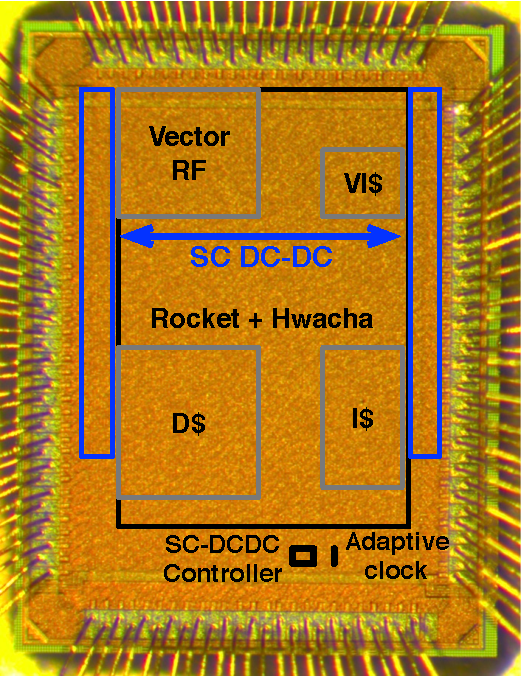
\includegraphics[width=0.6\textwidth]{6-raven3-diephoto}
  \caption{Annotated die micrograph of the Raven-3 testchip~\cite{Zimmer2016}.}
  \label{fig:6-raven3-diephoto}
\end{figure}



\subsection{Raven-4}

The Raven-4 testchip builds upon the Raven-3 design with design changes and additional features~\cite{Keller2017}.
The integrated voltage regulation and adaptive clocking systems are improved and supplemented with an integrated power management unit allowing fast adaptive voltage scaling (AVS) algorithms to be demonstrated on die.
An integrated body bias generator, power monitor, and measurement circuits enable more extensive power management and system characterization.
A block diagram of the testchip is shown in Figure~\ref{fig:6-raven4-blockdiagram}.

\begin{figure}
  \centering
  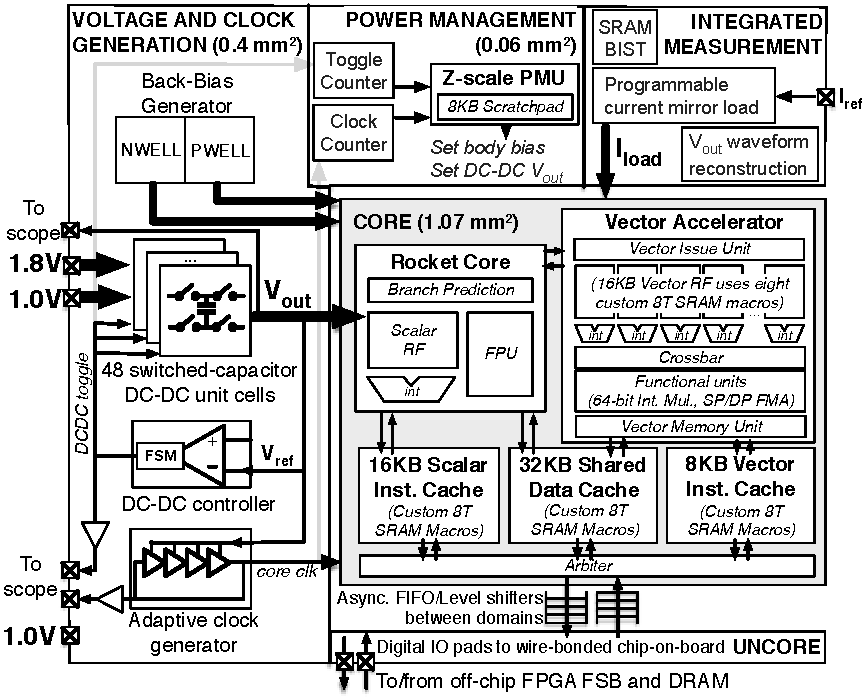
\includegraphics[width=\textwidth]{6-raven4-blockdiagram}
  \caption{A block diagram of the Raven-4 testchip~\cite{Keller2016} ({\textcopyright} 2016 IEEE, reprinted with permission).}
  \label{fig:6-raven4-blockdiagram}
\end{figure}

The core voltage domain contains an updated version of the Rocket core implemented in Raven-3.
The Hwacha vector accelerator is improved with the inclusion of additional math resources, doubling the peak rate of computation.
Additionally, separate long-latency functional units are dedicated to the coprocessor rather than being shared with the Rocket core.
The core SRAMs are implemented using the same custom 8T macros to enable low-voltage operation.
Level shifters and bisynchronous FIFOs guard the crossings to the uncore clock domain, which contains the PMU, control registers, IP, and IO logic.

The integrated voltage regulator and clocking systems that supply the core are also improved from Raven-3.
The flying capacitance of the SC regulators is doubled to forty-eight \SI{90}{\micro\meter} $\times$ \SI{90}{\micro\meter} unit cells, enabling improvements in conversion efficiency.
Decoupling capacitance was added to improve the integrity of the \SI{1.0}{\volt} and \SI{1.8}{\volt} inputs to the SC unit cells and help offset power delivery issues caused by the wirebond packaging of the chip.
%Custom decoupling cells with MOS capacitors and a six-layer MOM \SI{50}{\nano\meter} mesh add \SI{539}{\pico\farad} of capacitance to the \SI{1.8}{\volt} supply and \SI{802}{\pico\farad} of capacitance to the \SI{1.0}{\volt} supply.
An improved, free-running clock generator is implemented alongside the version employed in Raven-3 for direct measurement comparison.
Unlike the Raven-3 design, the replica timing circuit is comprised of multiple types of standard cells, each with an independently selectable depth.
%Large insertion delays diminish the effectiveness of adaptive clocking, so care was taken during physical design to reduce the insertion delay of the core clock tree compared to Raven-3.

A second, smaller processor serves as the power management unit (PMU) for the design.
The PMU processor is based on Z-scale, a tiny, three-stage RISC-V implementation that is nonetheless fully programmable via the RISC-V software toolchain.
The application core and the PMU can communicate directly via inter-processor interrupts, and each has a register mapped directly into the control and status register (CSR) space of the other system, allowing arbitrary data to be communicated between the two cores.
%Table~\ref{tab:raven4-processors} compares key features of the two processors.
The processor maps the control registers for the SC converters, adaptive clock generator, and other IP into its CSR space, which enables programs to directly manipulate the voltage and frequency of the chip.
In addition, the core clock and the SC toggle clock are read by counters, and the counter values are synchronized into the uncore domain.
Successive reads to this second counter enable a rapid estimate of core power consumption for active power management.

Several other circuits further the power management and measurement capabilities of the SoC.
The threshold voltage of the logic in the core voltage domain can be manipulated by an integrated body bias generator.
Fine tuning resolution and fast response allow adaptive body bias to be incorporated into power management techniques.
%Because the core voltage waveform is difficult to accurately observe off-chip due to parasitics on the measurement path, a waveform measurement circuit was implemented that uses a lightweight sampling approach to statistically reconstruct the waveform~\cite{Cochet2016}.
%This approach allows core power consumption to be measured with high accuracy via numerical integration.
%As the current load of the application core can vary over time and has a limited range, a programmable current-mirror load connected to the core voltage domain was added to allow straightforward characterization and measurement of the SS-SC converters and power monitoring circuitry.
The core clock and SS-SC toggle clock are also connected to output drivers for direct observation.

\begin{figure}
  \centering
  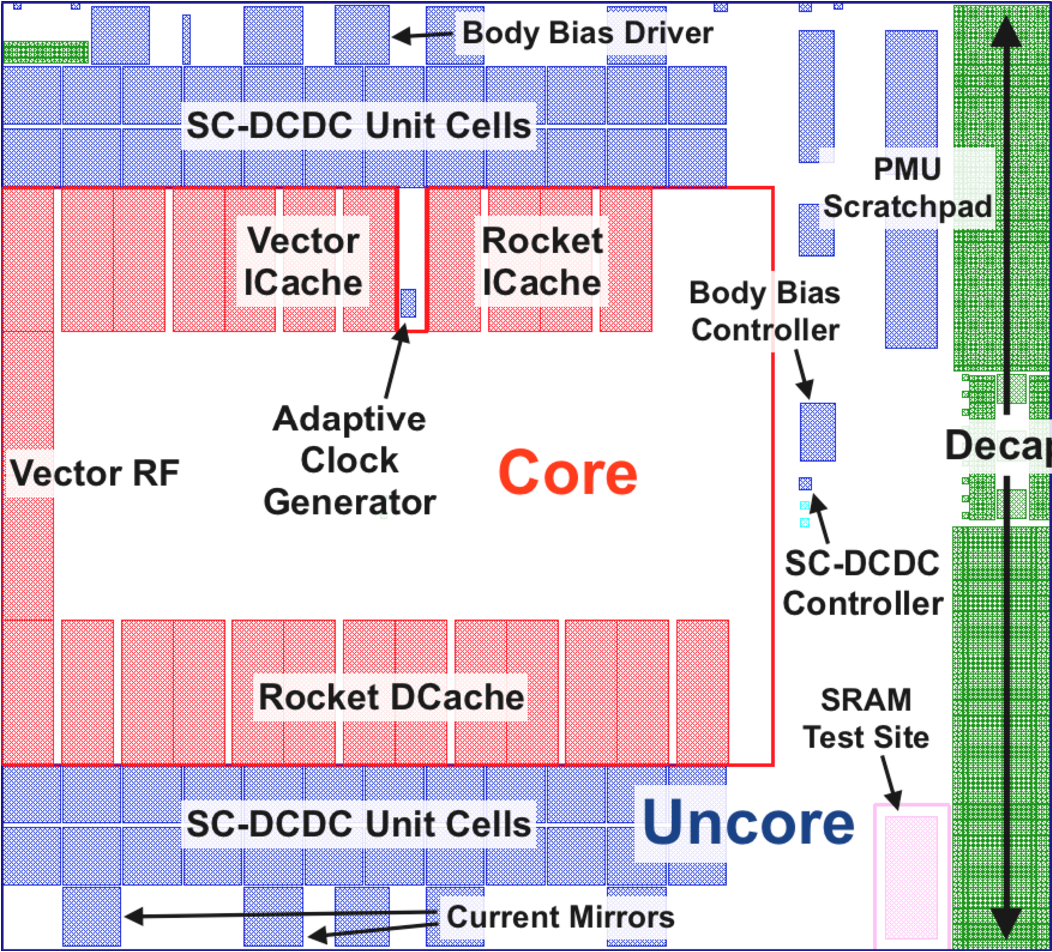
\includegraphics[width=0.6\textwidth]{6-raven4-floorplan}
  \caption{Annotated floorplan of the Raven-4 testchip~\cite{Keller2017} ({\textcopyright} 2017 IEEE, reprinted with permission).}
  \label{fig:6-raven4-floorplan}
\end{figure}

Figure~\ref{fig:6-raven4-floorplan} shows the floorplan of the SoC.
The design is partitioned into two voltage areas, with the core voltage area supplied by the SS-SC converters placed centrally.
Numerous additional voltages and clocks are defined to supply both the core and the various analog and mixed-signal blocks that make up the SoC.
To reduce core insertion delay, the clock generator itself was placed near the center of the core area, and a ``peninsula" of the uncore voltage domain was extended to allow the routing of control signals from the block to the top level of the design hierarchy.
The location of the core clock multiplexer, which allowed the selection of different core clock sources for test, was specified explicitly and placed near the center of the core area.
These improvements combined to reduce core insertion delay by several hundred picoseconds.
An annotated die photo of the testchip, which was fabricated in \SI{28}{\nano\meter} UTBB FD-SOI, is shown in Figure~\ref{fig:6-raven4-diephoto}.

%TODO - tweak figure
\begin{figure}
  \centering
  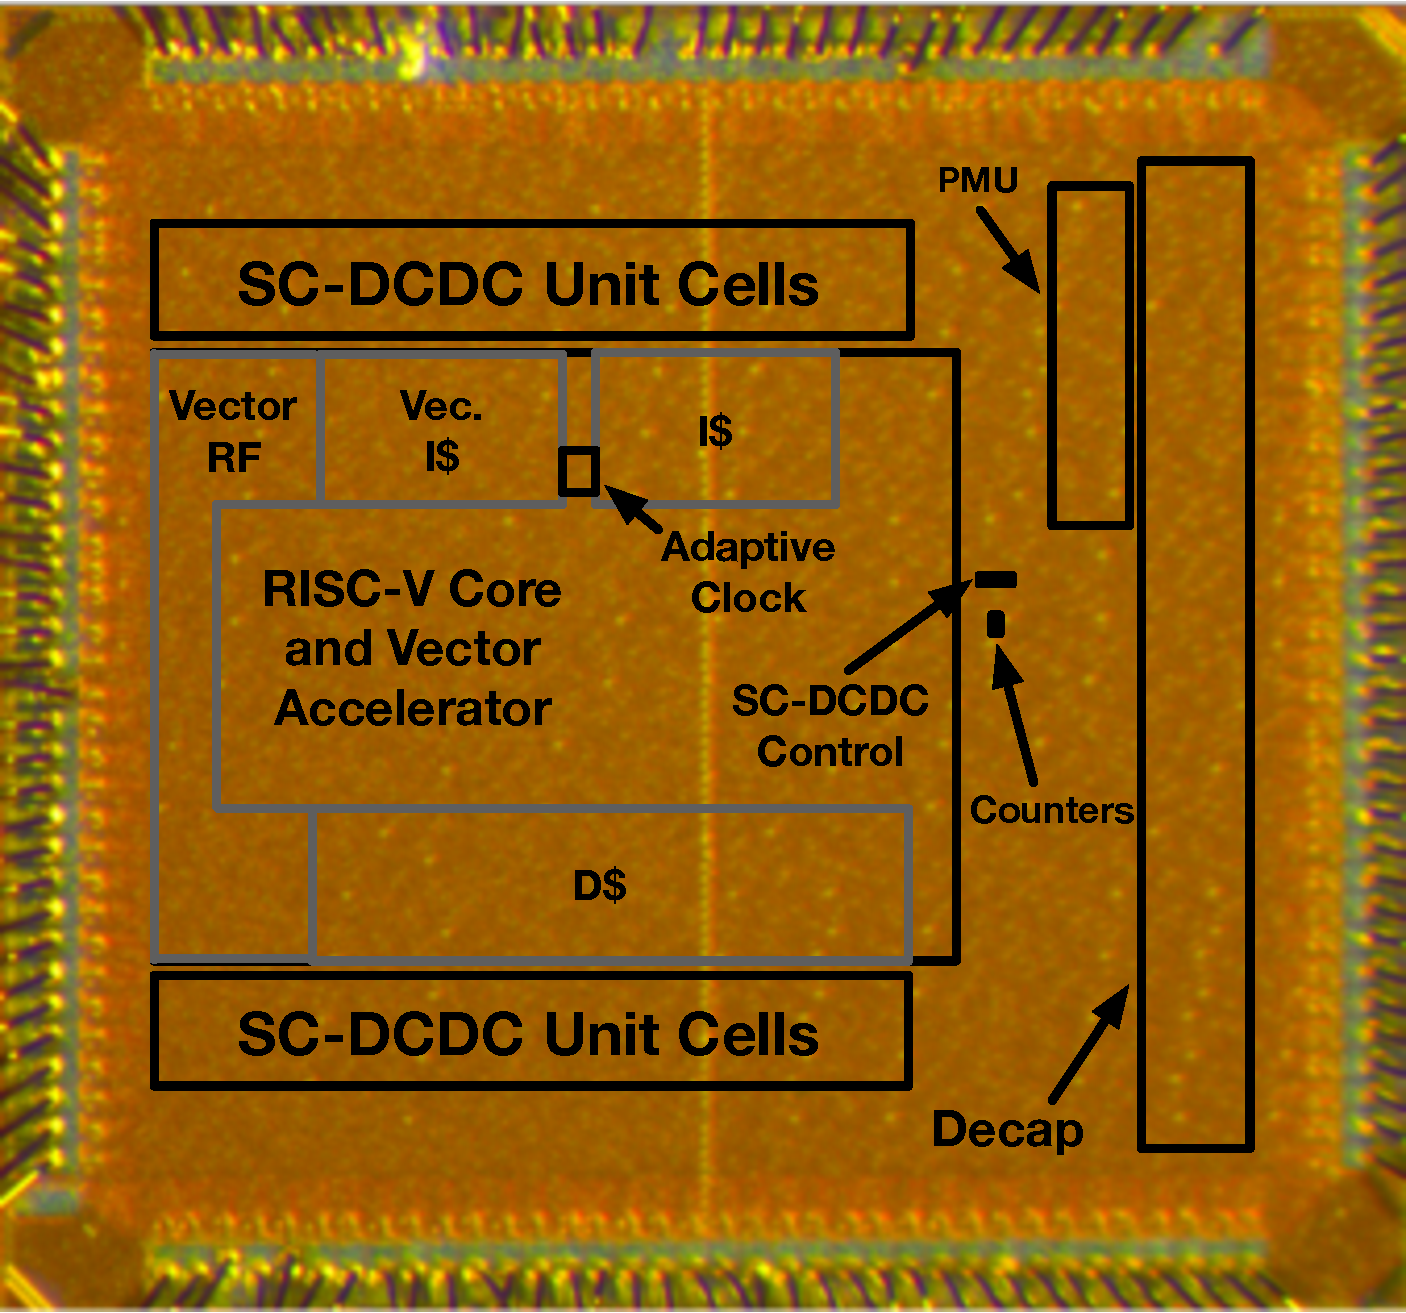
\includegraphics[width=0.6\textwidth]{6-raven4-diephoto}
  \caption{Annotated die micrograph of the Raven-4 testchip~\cite{Keller2016}.}
  \label{fig:6-raven4-diephoto}
\end{figure}



%-------------------------------------%
\section{RISC-V Processors}

The RISC-V instruction set was developed as a free and open architecture that defines simple base instructions and optional extensions~\cite{RISCV}.
Without licensing requirements, the ISA encourages experimentation and allows for the flexibility needed to design tightly-integrated FD-SOI systems.
Raven-3 and Raven-4 implement the Rocket scalar processor and the Hwacha vector accelerator.
In addition, Raven-4 implements a small Z-scale processor for power management.

\subsection{Rocket Chip}

Rocket Chip is a freely available in-order RISC-V implementation.
The processor, an instance of the Rocket Chip Generator~\cite{Rocket2016}, is a 64-bit five-stage single-issue pipeline (see Figure~\ref{fig:6-raven3-rocket}).
The pipeline is carefully designed to minimize the impact of long clock-to-output delays of SRAM macros.
For example, the pipeline resolves branches in the memory stage to shorten the critical path through the bypass path, but relies on extensive branch prediction (a 64-entry branch target buffer, a 256-entry two-level branch history table, and a two-entry return address stack) to mitigate the increased branch resolution penalty.
The blocking \SI{16}{\kibi\byte} instruction cache is private to the Rocket core, while the nonblocking \SI{32}{\kibi\byte} data cache is shared between the scalar core and a vector coprocessor designed to accelerate data-parallel workloads.
The Rocket core has a memory-management unit that supports page-based virtual memory.
Both caches are virtually indexed and physically tagged, and have separate TLBs that are accessed in parallel with cache accesses.
The core has an IEEE 754-2008-compliant floating-point unit that executes single- and double-precision floating-point operations, including fused multiply-add (FMA) operations, with hardware support for subnormal numbers.

%TODO - tweak figure
\begin{figure}
  \centering
  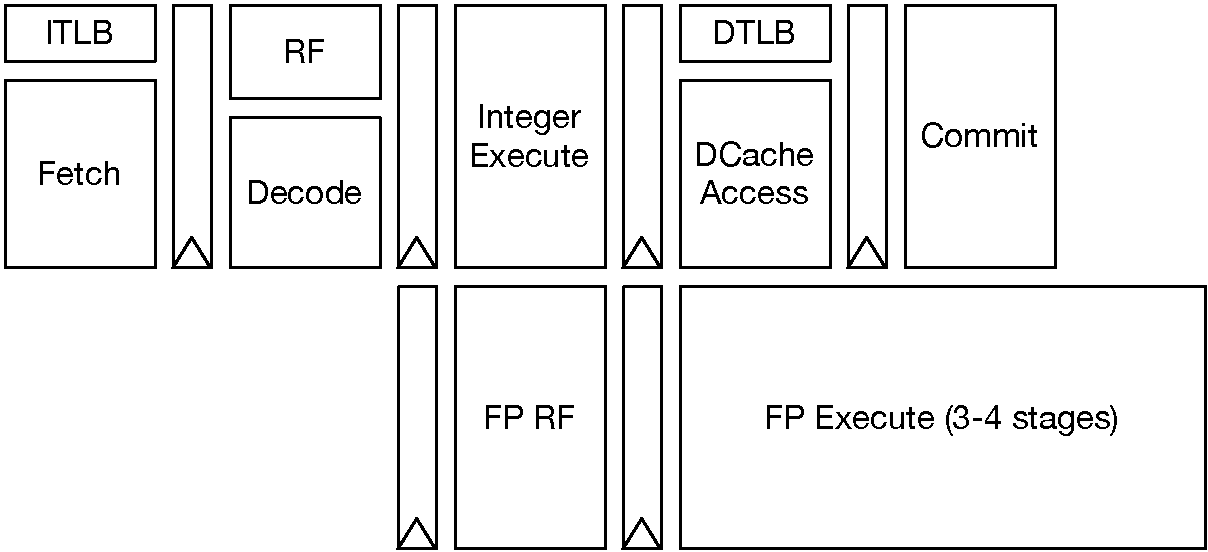
\includegraphics[width=0.8\textwidth]{6-raven3-rocket}
  \caption{A simplified pipeline diagram of the Rocket processor~\cite{Zimmer2016}.}
  \label{fig:6-raven3-rocket}
\end{figure}

%To reduce design complexity, the microprocessor is implemented as a tethered system.
%Unlike a standalone system, a tethered system depends on a host machine to boot, and lacks I/O devices such as a console, mass storage, frame buffer, and network card.
%The host (e.g., an x86 laptop) is connected to the target tethered system via the host-target interface (HTIF), a simple protocol that lets the host machine read and write target memory and control registers.
%All I/O-related system calls are forwarded to the host machine using HTIF, where they are executed on behalf of the target.
%Programs that run on the scalar core are downloaded into the target's memory via HTIF.
%The resulting system is able to boot modern operating systems such as Linux utilizing I/O devices residing on the host machine, and can run standard applications such as the Python interpreter.


\subsection{Hwacha Vector Processor}

The Hwacha vector accelerator, shown in Figure~\ref{fig:6-raven3-hwacha}, is a decoupled single-lane vector unit tightly coupled with the Rocket core that implements a custom RISC-V vector extension~\cite{Lee2014}.
Hwacha executes vector operations temporally (split across subsequent cycles) rather than spatially (split across parallel datapaths), and has a vector length register that simplifies vector code generation and keeps the binary code compatible across different vector microarchitectures with different numbers of execution resources.
The Rocket scalar core sends vector memory instructions and vector fetch instructions to the vector accelerator.
A vector fetch instruction initiates execution of a block of vector arithmetic instructions.
The vector execution unit (VXU) fetches instructions from the private \SI{8}{\kibi\byte} vector instruction cache (VI\$), decodes instructions, clears hazards, and sequences vector instruction execution by sending multiple micro-ops down the vector lane.
The vector lane consists of a banked vector register file built out of two-ported SRAM macros, operand registers, per-bank integer ALUs, and long-latency functional units.
Multiple operands per cycle are read from the banked register file by exploiting the regular access pattern with operand registers used as temporary space~\cite{Lee2014}.
%The long-latency functional units such as the integer multiplier and FMA units are shared between the Rocket core and the Hwacha accelerator.
The vector memory unit (VMU) supports unit-strided, constant-strided, and gather/scatter vector memory operations to the shared L1 data cache.
Vector memory instructions are also sent to the vector runahead unit (VRU) by the scalar core.
The VRU prefetches data blocks from memory and places them in the L1 data cache ahead of time to increase performance of vector memory operations executed by the VXU.
The resulting vector accelerator is more similar to traditional Cray-style vector pipelines~\cite{Russel1978} than SIMD units such as those that execute ARM's NEON or Intel's SSE/AVX instruction sets, and delivers high performance and energy efficiency while remaining area efficient.

%TODO - tweak figure
\begin{figure}
  \centering
  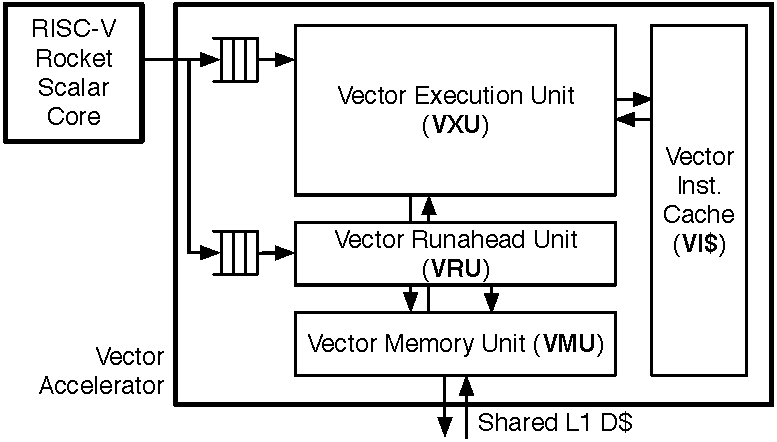
\includegraphics[width=0.65\textwidth]{6-raven3-hwacha}
  \caption{A block diagram of the Hwacha vector accelerator~\cite{Zimmer2016}.}
  \label{fig:6-raven3-hwacha}
\end{figure}


\subsection{Z-scale}

Z-scale is a 32-bit 3-stage single-issue in-order RISC-V processor (see Figure~\ref{fig:4-zscale}) that is suitable as a power management unit (PMU) due to its simplicity and small footprint.
The core forgoes caches in favor of an \SI{8}{\kibi\byte} 128-bit-wide scratchpad memory.
The PMU supports the RV32IM instruction extensions and is fully programmable via the RISC-V software toolchain.
It is designed to reside in a fixed-voltage ``always-on" domain for use in controlling the operating states of the remaining domains in the system.

%TODO - tweak figure
\begin{figure}
  \centering
  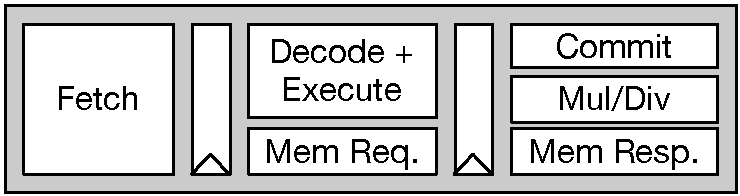
\includegraphics[width=0.5\textwidth]{4-zscale}
  \caption{The Z-scale processor pipeline~\cite{Keller2017}.}
  \label{fig:4-zscale}
\end{figure}

The three-stage design minimizes gate count while enabling sufficient performance to enable fine-grained power management.
The first stage of the pipeline fetches an instruction out of a 128-bit line buffer that reduces read-port contention on the single-ported scratchpad by storing four consecutive RISC-V instructions (the value of the program counter is calculated in the previous cycle).
The second stage of the pipeline decodes a RISC-V instruction, reads the register file, and executes an ALU instruction.
Branches are resolved in the second stage, so the instruction in the fetch stage is flushed when a branch is taken.
Writeback is isolated into the third stage of the pipeline, reducing the fanout delay on the write port of the register file.
The result in the third stage is bypassed to the second stage, eliminating the need for stalls in some cases.
The memory stage and the multiplication/division pipeline stages are also in the third pipeline stage, although only one of these three subsystems will be active at a time, as their use triggers a stall in the second stage until the result of the instruction is written back to the register file.
The multiply and divide units minimize hardware resources such that only one bit of the operation is completed each cycle, and so 32 cycles are required to compute any multiplication or division result.
Loads and stores directly access the scratchpad; since the scratchpad is 128 bits wide, the pipeline must properly swizzle the load data and store data.
An extra pipeline register was added in the arbiter between instruction and data memory requests to eliminate a long critical path and speed the achievable cycle time of the design.
The entire design (excluding the scratchpad memories) uses just 18K gates, making the implementation overhead small relative to large application processors, accelerators, and caches.
A comparison between the Rocket and Z-scale implementations in Raven-4 is shown in Table~\ref{tab:raven4-processors}.

\begin{table}[]
\footnotesize
\renewcommand{\arraystretch}{1.2}
\centering
\begin{tabular}{@{}lll@{}}
\toprule
\textbf{Feature} & \textbf{Rocket (excluding Hwacha)} & \textbf{Z-scale} \\
\midrule
{Instruction Set} & RISC-V RV64G & RISC-V RV32IM\\
{Pipeline} & Five-stage single-issue in-order & Three-stage single-issue in-order\\
{Memories} & 32KB DCache, 16KB ICache & 8KB unified scratchpad \\
{Standard Cell Count} & 196K & 18K \\
{Area (Cells + Memories)} & \SI{0.461}{\milli\meter}$^2$ & \SI{0.053}{\milli\meter}$^2$ \\
\bottomrule
\end{tabular}
\caption{Comparison of the two Raven-4 processors~\cite{Keller2017}.}
\label{tab:raven4-processors}
\end{table}


%For fast power-management feedback loops, it is critical that the PMU be able to read counters and actuate changes in voltage and frequency with low latency.
%The Z-scale PMU accomplishes this by mapping all system control registers, including both counters used to sense activity changes and control registers used to change the operating condition of a voltage domain, into its control status register (CSR) space, so that reading or writing from these registers accesses the appropriate system registers directly in hardware.
%CSR reads and writes are natively supported in the RISC-V ISA, so standard instructions can be used to write programs for power management.
%An alternative implementation memory-maps all system control registers, allowing the PMU core to access key system state with standard load and store operations.


%-------------------------------------%
\section{Energy-Efficient SRAMs}

Operation at low voltages is critical to achieving maximum energy efficiency, but on-chip SRAM typically limits the minimum operating voltage of the entire system as the small transistors in SRAM bitcells are especially vulnerable to process variation.
Raven-3 and Raven-4 implement custom 2KB 8T-based SRAM macros as shown in Figure~\ref{fig:sram}.
It is logically organized as 512 entries of 72 bits (64 bits + 8 possible ECC bits) and physically organized as two arrays of 128 rows by 144 columns with two-to-one physical interleaving.
Low-voltage operation is enabled by the 8T bitcell, where each transistor is larger than the equivalent high-density 6T bitcell, and by the FD-SOI process which reduces the threshold voltage variation \cite{planes}~\cite{raven1}.
While the arrays also implemented a negative bitline write assist, the assist was not necessary to achieve minimum voltage operation.

\begin{figure}
  \centering
  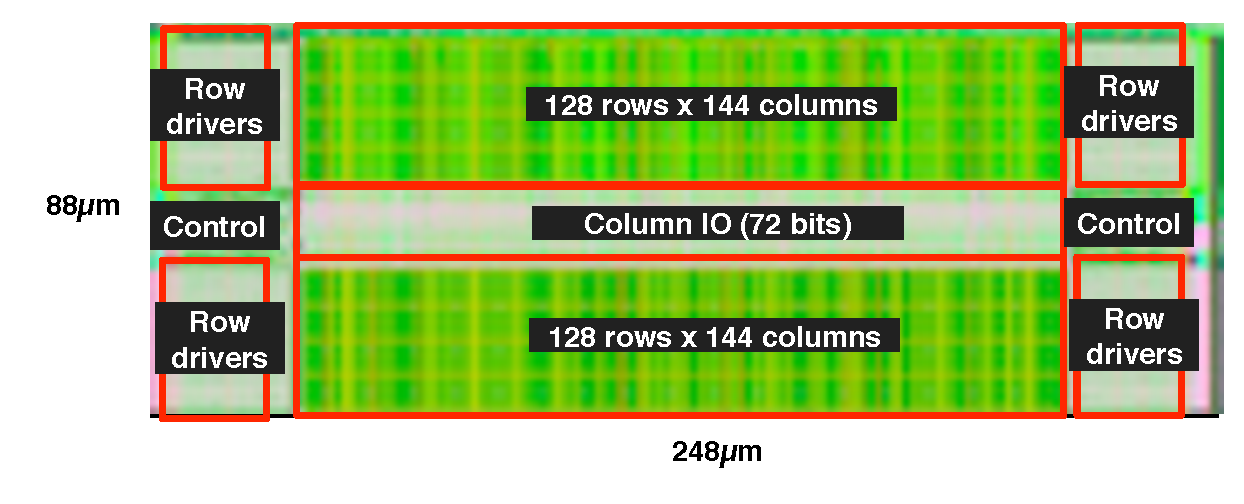
\includegraphics[width=0.7\textwidth]{sram}
  \caption{Layout of the custom 8T SRAM macro~\cite{Keller2017} ({\textcopyright} 2017 IEEE, reprinted with permission).}
  \label{fig:sram}
\end{figure}


%-------------------------------------%
\section{DC-DC Converters}
\label{sec:sc-dcdc}

The implementation of AVS to improve system energy efficiency requires the delivery of multiple different voltages to different areas of the chip, and the particular voltages used must be dynamically reconfigurable.
These multiple voltages are supplied by voltage regulators, circuits that convert one voltage to another.
Typically, one or two input voltages will be downconverted by one or more voltage regulators to some number of lower voltages for use by the different voltage areas of the SoC.
By building regulators into the same die as the SoC they are supplying, system costs are reduced, transition times are shortened due to the smaller passives, and many voltages can be generated from just a few external supplies, ameliorating any issues with IO count.
However, integrated regulators must achieve high conversion efficiency while minimizing area overhead.

%All \SI{1}{\volt} input switches are implemented as low-$V_t$ devices to reduce their \textsc{on} resistance, while the larger \SI{1.8}{\volt} input switches are implemented as regular-$V_t$ devices with FBB applied to further reduce their leakage when active.
%To achieve simultaneous switching, the DCDC toggle clock generated by the controller must arrive at each unit cell at the same time.
%The place-and-route tool was therefore directed to construct a clock tree for this signal, balancing arrival times.
%The flying capacitor is implemented using MOS capacitors with two layers of MOM capacitors above.
%Parasitic bottom-plate capacitance is reduced by using a series connection of the box, well, and substrate capacitances~\cite{Le2013}.
%The converter achieves a total capacitance of \SI{2.1}{\nano\farad} and a capacitive density of \SI{11.0}{\femto\farad\per\micro\meter\squared}. 

Switched-capacitor voltage regulators are a favorable choice for integrated voltage regulation because high-quality integrated capacitors are much easier to implement than inductors, while switching regulator efficiencies exceed those of linear regulators.
However, switched-capacitor regulators typically achieve conversion efficiencies that are not high enough to justify their overhead. 
%Energy savings from AVS are reduced by conversion losses to the extent that the additional area and design complexity required for their implementation were not worthwhile.
Designing a switched-capacitor regulator with reasonably high efficiency is a critical component of a realistic FG-AVS system.

Because each switching event in a switched-capacitor circuit is perturbing its output voltage with a discontinuous addition of charge, the output of switched-capacitor regulators tends to ripple.
Traditional switched-capacitor designs employ a technique known as interleaving to suppress this voltage ripple and produce a relatively flat output supply that is well-suited for synchronous digital logic \cite{Clerc2015, Jain2014, Jiang2017, Kim2015, Song2015, Teh2016}.
By dividing the total flying capacitance in the system into many smaller unit cells, and switching each of these unit cells out of phase with the others, the relative amount of charge delivered onto the supply with each switching event is small, and the output voltage ripple is minimized as shown in Figure~\ref{fig:3-simultaneous-switching-a}.
High interleaving phase counts of 16, 32, or even greater can be used to suppress the ripple and produce a steady output voltage \cite{Andersen2014, Le2011, Pique2012}.
However, this interleaved approach suffers from charge-sharing losses as each unit cell shares charge across the flying capacitance of the others when it switches.
These intrinsic charge-sharing losses comprise up to 40\% of the overall energy losses in the voltage conversion~\cite{Jevtic2014}.

\begin{figure}
  \centering
  \hspace*{\fill}
  \begin{subfigure}[t]{0.42\textwidth}
  \centering
  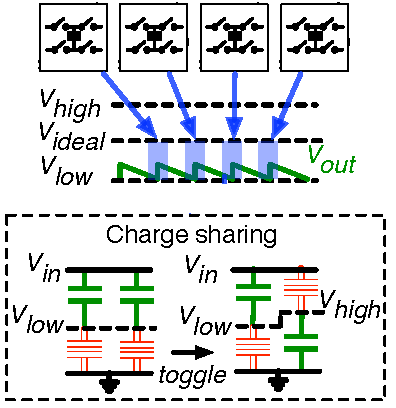
\includegraphics[width=\textwidth]{3-simultaneous-switching-a}
  \caption{}
  \label{fig:3-simultaneous-switching-a}
  \end{subfigure}
  \hspace*{\fill}
  \begin{subfigure}[t]{0.42\textwidth}
  \centering
  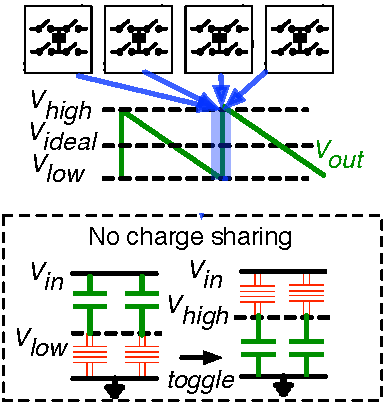
\includegraphics[width=\textwidth]{3-simultaneous-switching-b}
  \caption{}
  \label{fig:3-simultaneous-switching-b}
  \end{subfigure}
  \hspace*{\fill}
  \caption{Interleaved and simultaneous-switching switched-capacitor DC-DC converters~\cite{Zimmer2016}.  In the four-phase interleaved converter shown in (\subref{fig:3-simultaneous-switching-a}), each unit cell switches out of phase with the others, resulting in a relatively flat output voltage but incurring charge-sharing losses.  In the simultaneous-switching converter shown in (\subref{fig:3-simultaneous-switching-b}), all unit cells switch at once, eliminating charge-sharing losses but resulting in a large output voltage ripple.}
  \label{fig:3-simultaneous-switching}
\end{figure}

The conversion losses of switched-capacitor voltage regulators are composed of four parts, three of which depend on the switching frequency of the design~\cite{Le2011}.
The intrinsic charge-sharing loss $P_{cfly}$ of switched-capacitor designs is inversely proportional to the switching frequency of the design, because a slower switching frequency means more charge being transferred for each switching event.
The bottom-plate conduction loss $P_{bottom}$ caused by the parasitic capacitance of the flying capacitor to ground and the parasitic gate capacitance $P_{gate}$ of the switches are both directly proportional to the switching frequency.
The conduction loss $P_{cond}$ through the switches does not depend on switching frequency.
Switched-capacitor designs typically operate at the optimal switching frequency to minimize the total losses in the system, operating fast enough to reduce charge-sharing losses but not so fast that the parasitic losses dominate.

%\subsection{Simultaneous-Switching Switched-Capacitor Regulation}
%\label{sec:3-sc-dcdc}

An alternative approach called simultaneous switching is shown in Figure~\ref{fig:3-simultaneous-switching-b}.
Instead of interleaving the unit cells, the entire flying capacitance of the regulator is switched at once, eliminating all charge-sharing between different unit cells present in the interleaved approach~\cite{Zimmer2016}.
The elimination of this loss term also means that the only losses remaining in the system are either directly proportional to switching frequency or agnostic to it, so the switching frequency of the system can be reduced, further shrinking remaining losses.
Figure~\ref{fig:3-dcdc-analysis} shows analytical results comparing the losses from an interleaved system with those of a simultaneous-switching regulator driving an ideal resistive load.
The simultaneous-switching switched-capacitor DC-DC (SS-SC) converter is able to achieve total losses of less than 10\% by slowing its switching frequency.
In real systems, the load is not purely resistive, but instead has some capacitive component, so charge-sharing losses are not eliminated entirely.
%Figure~\ref{fig:3-dcdc-analysis-cap} shows a simulated example of how the inclusion of a capacitive load in the SS-SC circuit diminishes some of the advantage of the simultaneous-switching design and increases the most efficient switching frequency relative to a purely resistive load.
Nonetheless, the energy savings over the interleaved approach remain substantial, and the optimal switching frequency is lower in the SS-SC design.

\begin{figure}
  \centering
  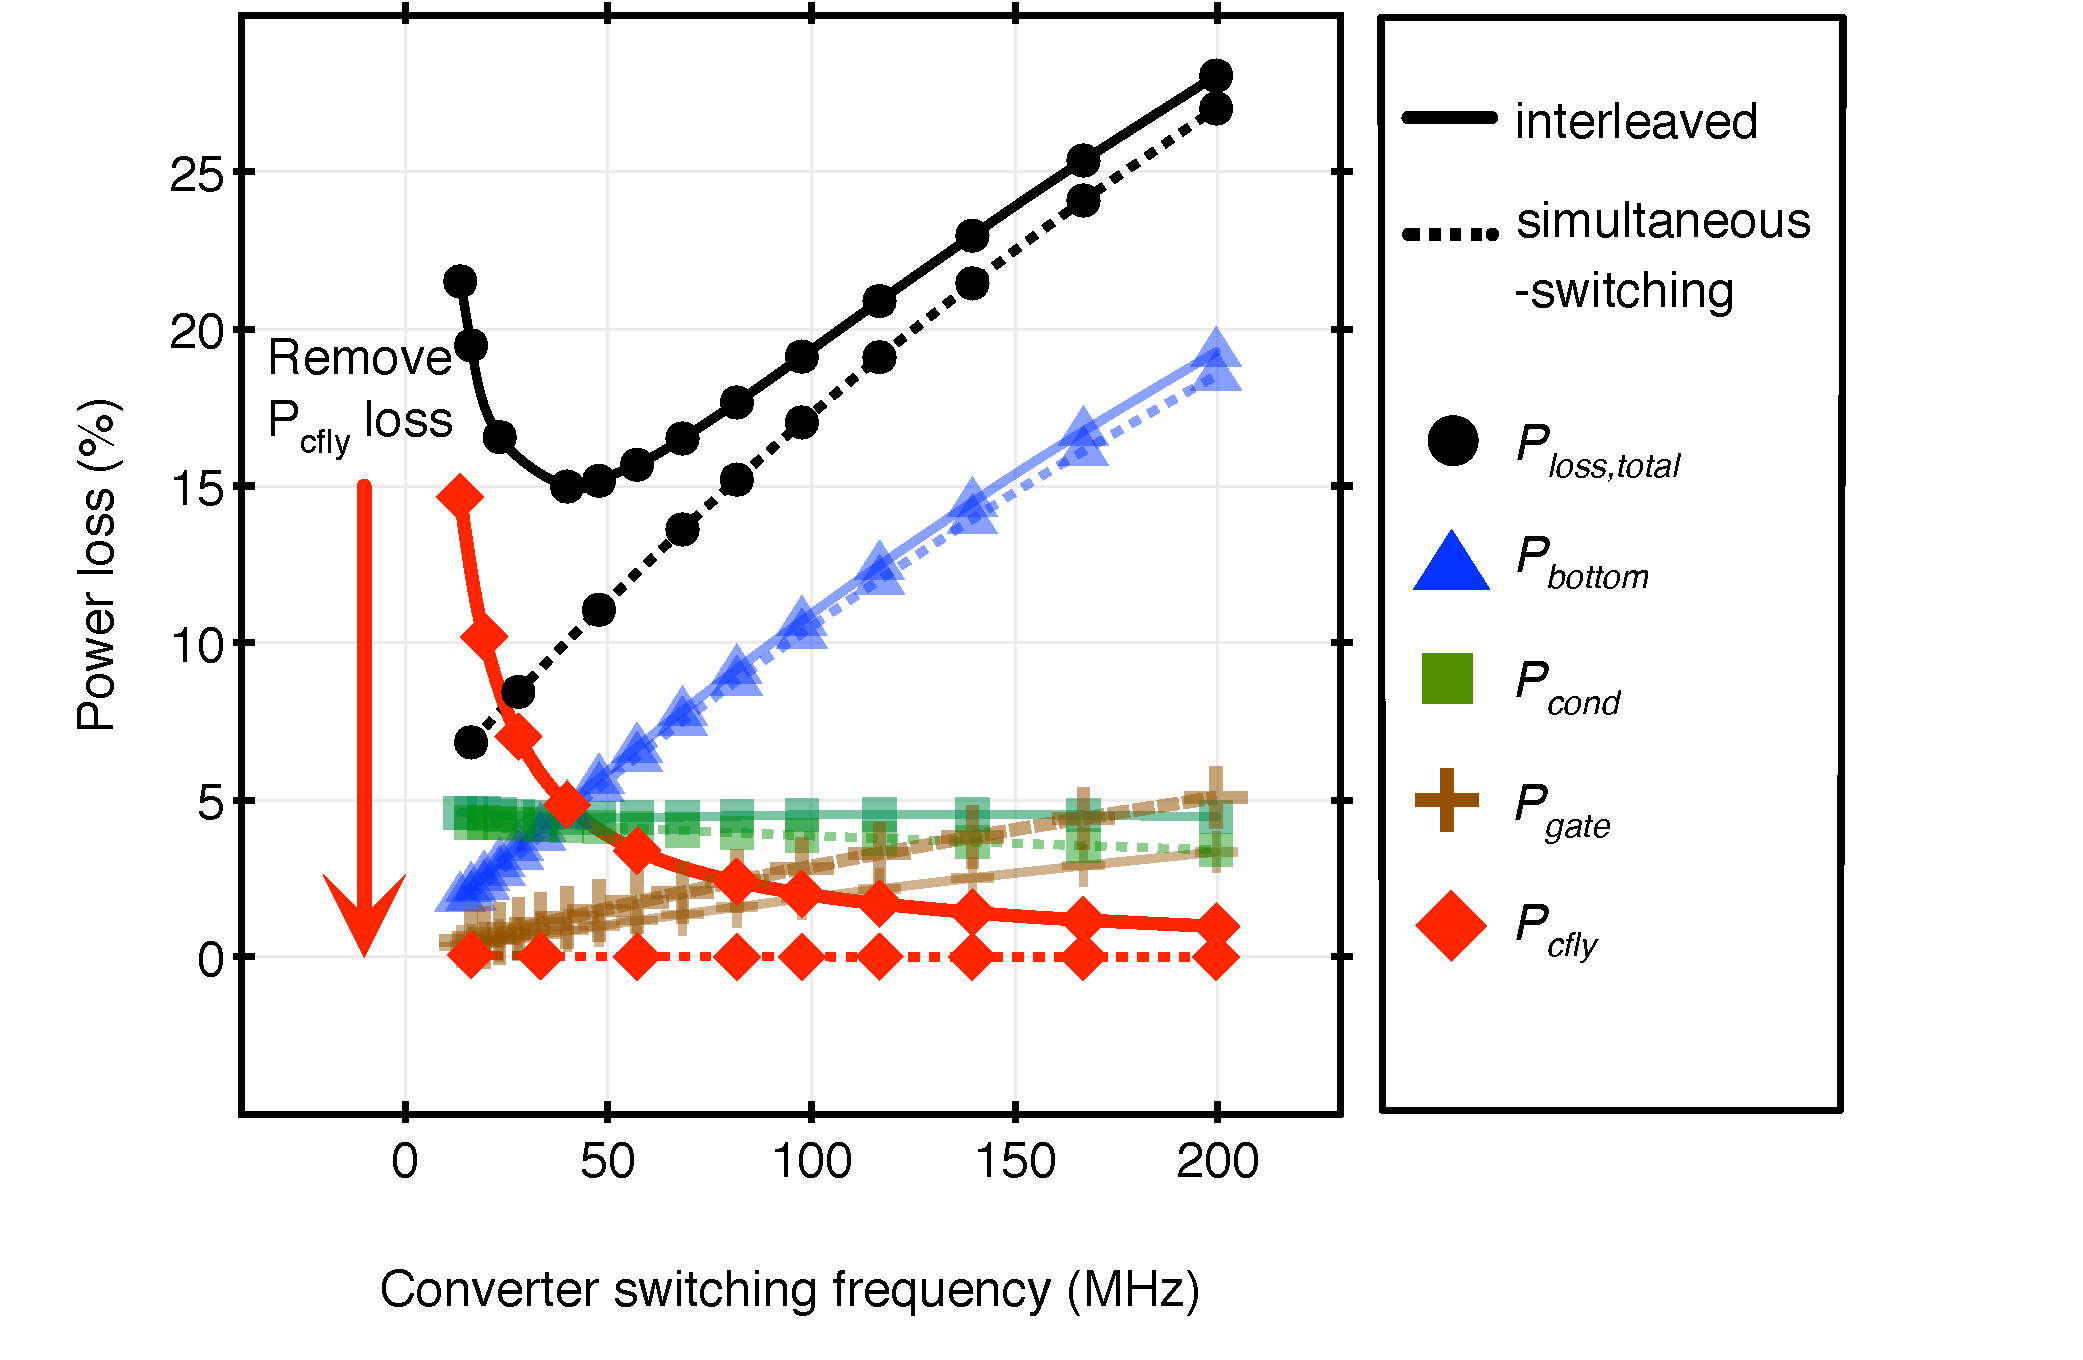
\includegraphics[width=0.8\textwidth]{3-dcdc-analysis}
  \caption{Analytical results showing the efficiency improvement of the simultaneous-switching switched-capacitor voltage regulator~\cite{Zimmer2016} ({\textcopyright} 2016 IEEE, reprinted with permission).}
  \label{fig:3-dcdc-analysis}
\end{figure}

%\begin{figure}
%  \centering
%  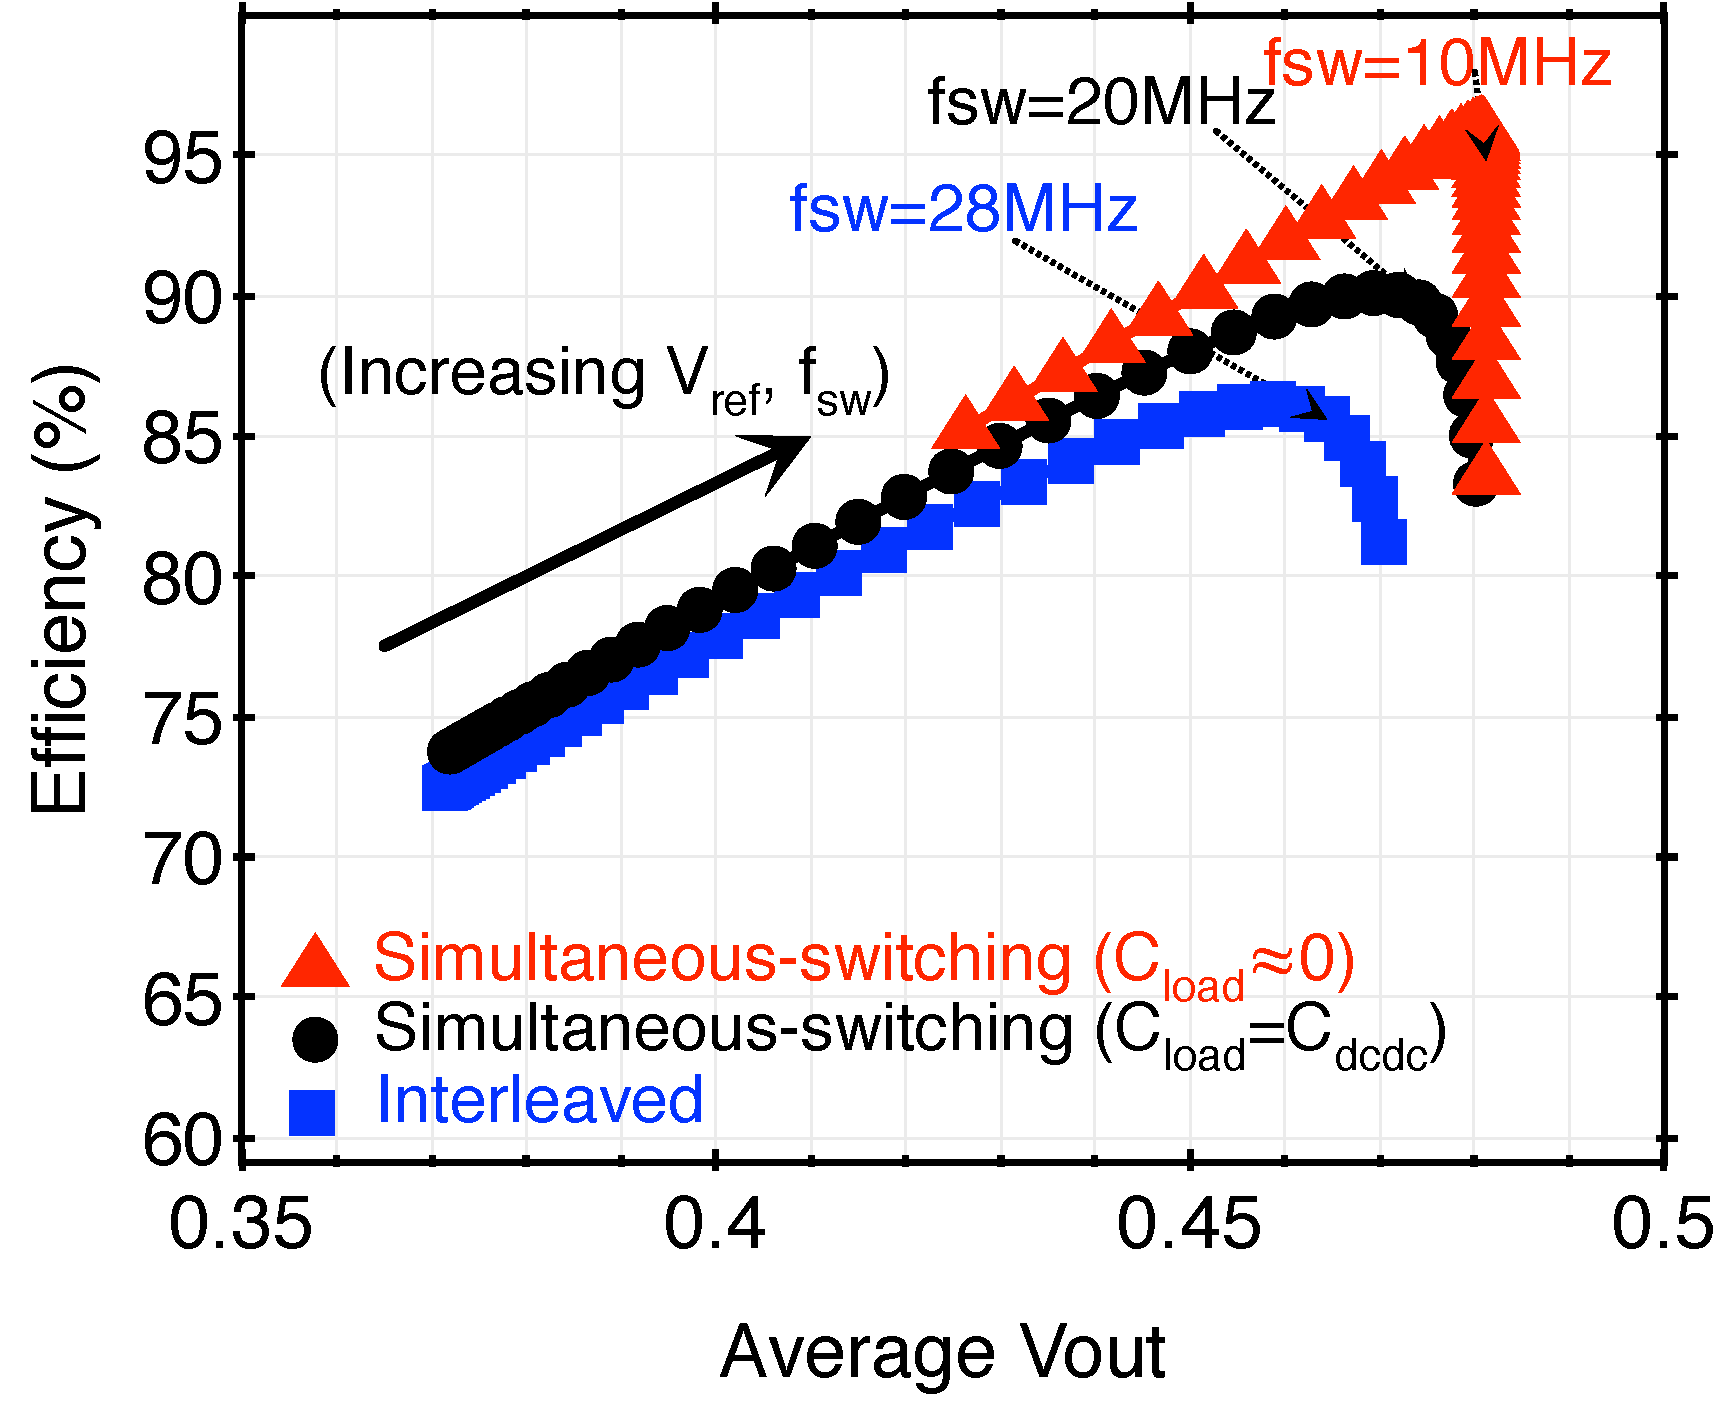
\includegraphics[width=0.6\textwidth]{3-dcdc-analysis-cap}
%  \caption{Simulation results showing the impact of load capacitance on converter efficiency and switching frequency~\cite{Zimmer2016} ({\textcopyright} 2016 IEEE).}
%  \label{fig:3-dcdc-analysis-cap}
%\end{figure}

Simultaneous-switching designs reduce the loss components associated with switched-capacitor regulation, but they generate an output voltage that ripples substantially around an average.
This rippling supply is not well-suited to a traditional synchronous digital system operating at a fixed clock frequency, because the digital clock must operate at a slower frequency corresponding to the lowest voltage of the ripple in order to guarantee safe operation.
This would result in wasted energy as the rippling voltage exceeds its minimum, as shown in Figure~\ref{fig:3-ripple-clocking-a}, and these over-voltage losses would exceed the savings from the elimination of charge sharing.
Systems employing SS-SC regulators therefore require the clock supplied to the digital load to adapt to the changing voltage in order to achieve reasonable efficiencies~\cite{Jevtic2014}.
As shown in Figure~\ref{fig:3-ripple-clocking-b}, by changing the clock on a cycle-by-cycle basis to match the instantaneous operating conditions of the load, the over-voltage losses can be eliminated.
Raven-3 and Raven-4 each implement this combination of simultaneous-switching conversion and adaptive clocking.

\begin{figure}
  \centering
%  \hspace*{\fill}
  \begin{subfigure}[t]{0.6\textwidth}
  \centering
  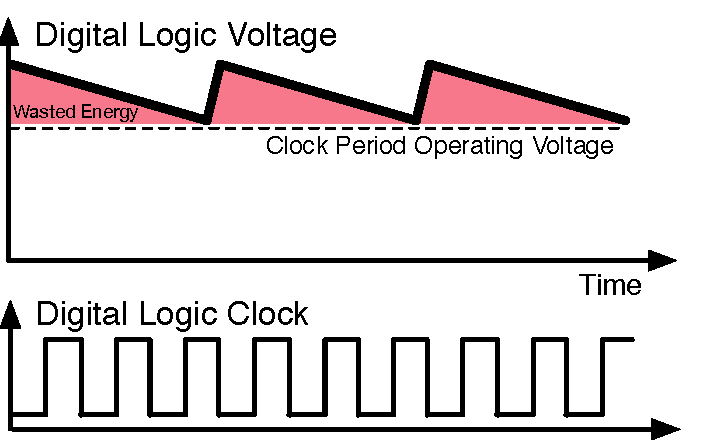
\includegraphics[width=\textwidth]{3-ripple-clocking-a}
  \caption{}
  \label{fig:3-ripple-clocking-a}
  \end{subfigure}
%  \hspace*{\fill}
  \par\bigskip
  \begin{subfigure}[t]{0.6\textwidth}
  \centering
  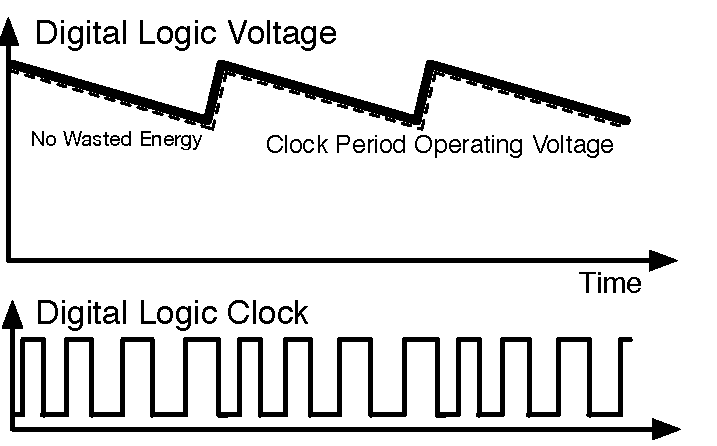
\includegraphics[width=\textwidth]{3-ripple-clocking-b}
  \caption{}
  \label{fig:3-ripple-clocking-b}
  \end{subfigure}
%  \hspace*{\fill}
  \caption{Sample voltage and clock waveforms of SS-SC systems.  In (\subref{fig:3-ripple-clocking-a}), the clock does not adapt to the voltage ripple, so it must be margined for the lowest supply voltage, resulting in wasted energy at higher voltages.  In (\subref{fig:3-ripple-clocking-b}), the clock adapts to the voltage ripple, allowing the circuit to speed up when the voltage is higher than the minimum.}
  \label{fig:3-ripple-clocking}
\end{figure}
 
Traditional switched-capacitor regulators achieve peak efficiencies when supplying output voltages at discrete levels determined by their topology.
While SS-SC regulators do not generate a fixed output voltage, their efficiency still peaks at a particular average output level.
As a wide range of voltages are desirable for FG-AVS, a reconfigurable switching network with a topology similar to that of \cite{Le2011} was implemented.
The design can operate in four different modes that generate voltages from fixed \SI{1}{\volt} and \SI{1.8}{\volt} supplies.
The \SI{1.8}{\volt} 1/2 mode downconverts the \SI{1.8}{\volt} input in a 2:1 ratio, resulting in an average output voltage around \SI{900}{\milli\volt}.
The \SI{1}{\volt} 2/3 mode and \SI{1}{\volt} 1/2 mode each downconvert the 1.0V input, resulting in average output voltages of roughly \SI{667}{\milli\volt} and \SI{500}{\milli\volt} respectively.
A bypass mode connects the \SI{1}{\volt} input directly to the output rail.
The design re-uses the flying capacitance and switches, reconfiguring the switching pattern between each topology to avoid area overhead (see Figure~\ref{fig:3-dcdc-topologies}).

\begin{figure}
  \centering
  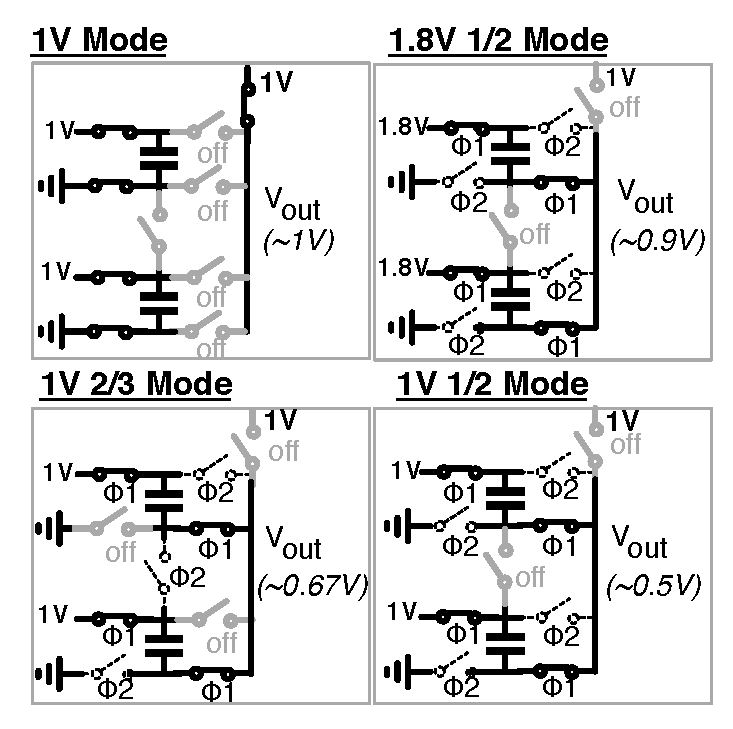
\includegraphics[width=0.6\textwidth]{3-dcdc-topologies}
  \caption{The four topologies of the reconfigurable SS-SC converter~\cite{Zimmer2016} ({\textcopyright} 2016 IEEE, reprinted with permission).}
  \label{fig:3-dcdc-topologies}
\end{figure}

The phases and configurations of the switches in the SS-SC regulator are set by a finite-state-machine controller.
This logic is responsible for configuring and reconfiguring the topology of the regulator, as well as switching between the two operating phases to pump charge onto the output of the converter.
The regulator topology is determined by setting a control register that, when changed, triggers a reconfiguration between voltage modes.
To generate the toggle clock that is distributed to the switches in the regulator, a comparator circuit acting on a \SI{2}{\GHz} clock detects when the regulated output voltage drops below a fixed external reference.
When the comparator triggers, control logic produces the next toggle clock edge, switching the SS-SC toggle clock phase and causing more charge to be supplied, boosting the voltage.
As a different reference voltage is needed for each mode, different comparators must be implemented to function in the appropriate voltage ranges (see Figure~\ref{fig:3-dcdc-comparators}).
In the event that one switching event does not sufficiently increase the generated voltage to bring it above the reference voltage, additional logic triggers further switching events after a delay, ensuring that the voltage will eventually be boosted back up to nominal levels.
%The state machine controller is diagrammed in Figure~\ref{fig:3-dcdc-state-machine}.

\begin{figure}
  \centering
  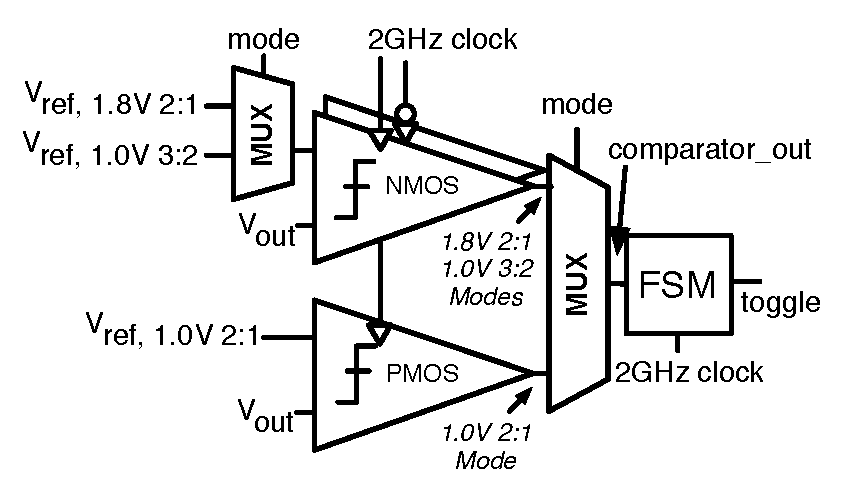
\includegraphics[width=0.6\textwidth]{3-dcdc-comparators}
  \caption{A diagram of the comparators used in the SS-SC controller~\cite{Zimmer2016} ({\textcopyright} 2016 IEEE, reprinted with permission).  Different comparators are needed to accommodate the voltage ranges of the references for the three different switching modes.}
  \label{fig:3-dcdc-comparators}
\end{figure}

%\begin{figure}
%  \centering
%  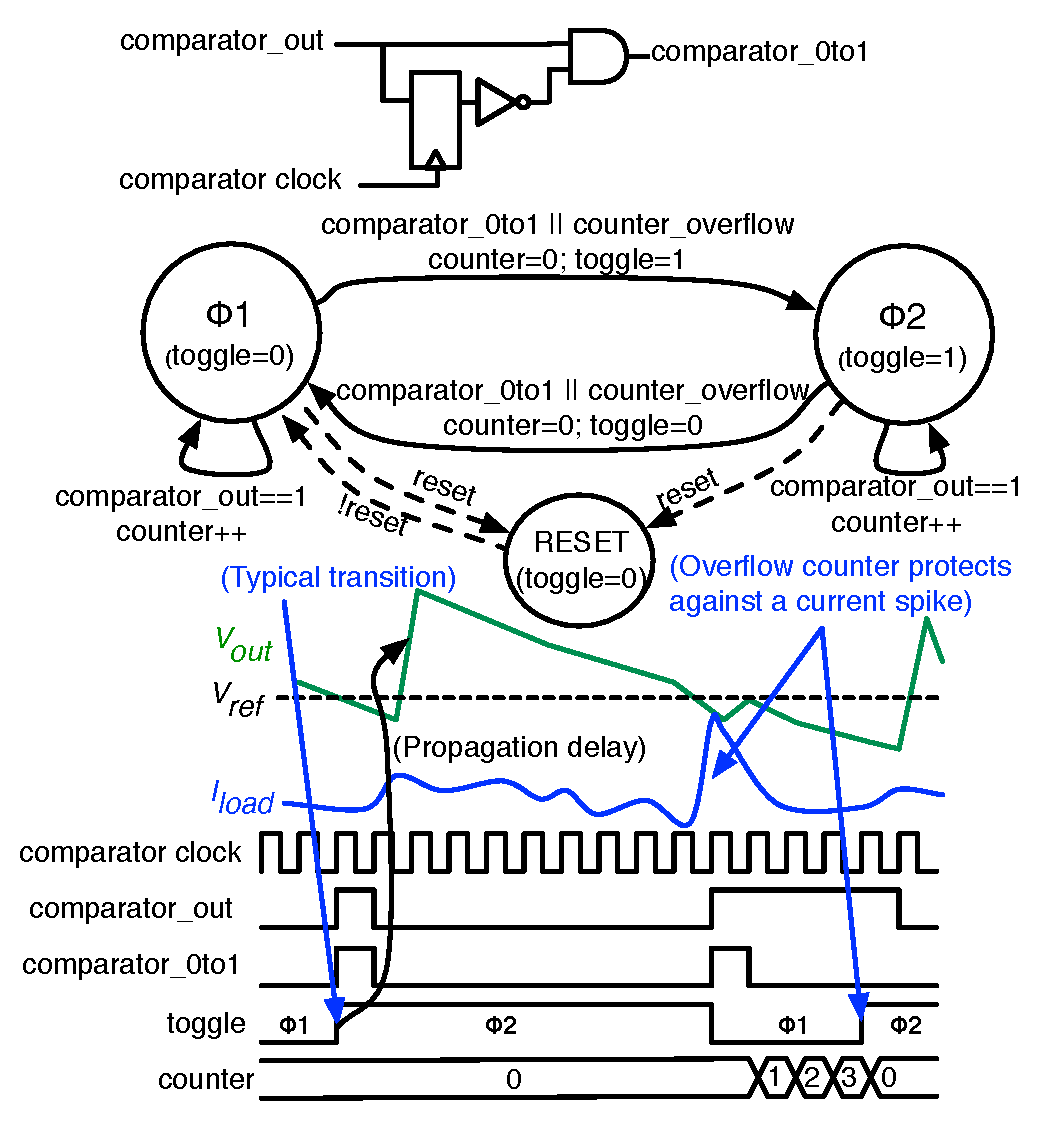
\includegraphics[width=0.8\textwidth]{3-dcdc-state-machine}
%  \caption{The state machine used in the SS-SC controller and example waveforms of its operation~\cite{Zimmer2016} ({\textcopyright} 2016 IEEE).  If the current demand increases as the converter is toggling, the voltage may not rise about $V_{ref}$, so an additional counter triggers further switching until the voltage increases.}
%  \label{fig:3-dcdc-state-machine}
%\end{figure}

%-------------------------------------%
\section{Body-Bias Generation}

The ultra-thin body and box (UTBB) FDSOI technology features a high sensitivity (>70mV/V) of transistor threshold voltages to body bias.
Forward well bias further lowers the thresholds and offers the opportunity for trading off active for leakage power for overall energy efficiency.
Optimal body bias can be used for run-time compensation of process, aging, temperature and supply-voltage variations, and to improve energy efficiency.

In contrast to adaptive voltage scaling (AVS), enabling adaptive body-bias (ABB) requires only two additional power grid lines.
The load for body biasing is almost purely capacitive with low static current.
Optimal body bias can be used for run-time compensation of process, aging, temperature and supply-voltage variations, or to improve energy efficiency~\cite{Tschanz2002}, but a compact, low power, fast body-bias generator (BBG) is required.
Raven-4 implements a fully-integrated switched-capacitor solution with a fine voltage step and sub-100ns response time that enables fast, fine-granularity threshold control~\cite{Blagojevic2016}.

The block diagram of the body-bias generator is shown in Figure~\ref{fig:bbgen-blockdiagram}, illustrating its two main modules, the controller and the driver unit.
The control unit contains a body voltage sensor and control logic.
Multiple drivers are placed across the chip to provide rapid response.
The controller has two main operating modes: transition or ON-mode, and keep-the-value or STEADY-mode.
In the ON-mode, a body bias sensor is employed.
This is a direct voltage sample-and-compare circuit clocked at 1 or 2GHz, enabling sub-ns closed loop control over the driver units.
A p-well sampler employs a -1:0.8 switched capacitor structure with 20\% gain-error to compensate for the lower PMOS body factor.
The outputs of the analog upper- and lower-bound rail-to-rail comparators are used to generate mutually exclusive charge or discharge commands.

\begin{figure}
  \centering
%  \hspace*{\fill}
  \begin{subfigure}[t]{0.6\textwidth}
  \centering
  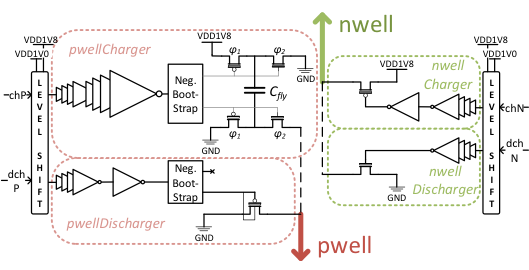
\includegraphics[width=\textwidth]{bbgen-blockdiagram-a}
  \caption{}
  \label{fig:bbgen-blockdiagram-a}
  \end{subfigure}
%  \hspace*{\fill}
  \par\bigskip
  \begin{subfigure}[t]{0.6\textwidth}
  \centering
  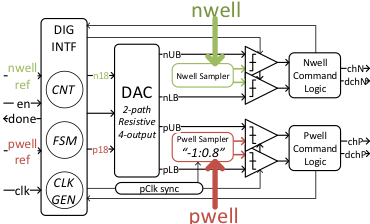
\includegraphics[width=\textwidth]{bbgen-blockdiagram-b}
  \caption{}
  \label{fig:bbgen-blockdiagram-b}
  \end{subfigure}
%  \hspace*{\fill}
  \caption{Block diagrams of the controller (\subref{fig:bbgen-blockdiagram-a}) and driver (\subref{fig:bbgen-blockdiagram-b}) of the integrated body-bias generator~\cite{Blagojevic2016} ({\textcopyright} 2016 IEEE, reprinted with permission).}
  \label{fig:bbgen-blockdiagram}
\end{figure}

Once the voltages settle inside the bounds, the control unit switches to low-power STEADY-mode and a 0.5MHz clock.
The analog reference voltages are generated with 5-bit two-path poly-resistor DACs in the slow path and a combination of MOS and poly resistors in the fast path.
This enables 2ns settling of the new upper-bound/lower-bound values and only 400nA of DAC static consumption in STEADY-mode.
The size of upper-bound/lower-bound window is programmable with a default value of 58mV.
When new digital target values are received, or when voltages leak out of the window, the fast clock unit is engaged within a cycle and the control unit switches into ON-mode to set new body-bias voltages.

The driver units receive four 1-bit digital commands from the control unit to toggle the charging and discharging of the transistor wells.
The n-well drivers are PMOS and NMOS power switches that provide 0V-1.8V range and high slew rates.
Figure~\ref{fig:bbgen-negative-vgen} shows the negative voltage generator needed for the p-well, which is based on a switched-capacitor (SC) charge-pump.
The driver implements a 1: 1 SC charge pump with a negative bootstrap circuit for the negative gate drive signal $G_{bot}$~\cite{Tsukikawa1993}
The flying capacitor consists of a MOS/MOM stack and occupies the lowest five metal layers to achieve 8fF/?m2 density at 1.8V.
The driver unit design enables straightforward distribution across large body bias domains for a fast and uniform charging profile.

\begin{figure}
  \centering
  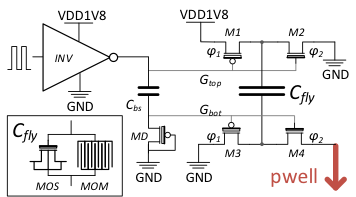
\includegraphics[width=0.6\textwidth]{bbgen-negative-vgen}
  \caption{The negative voltage generator used to generate p-well voltages~\cite{Blagojevic2016} ({\textcopyright} 2016 IEEE, reprinted with permission).}
  \label{fig:bbgen-negative-vgen}
\end{figure}

%-------------------------------------%
\section{Clock Generation}

Because SS-SC converters generate a rippling supply voltage, only a clock that adjusts to this ripple on a cycle-by-cycle basis to supply the digital logic can avoid wasted energy in these systems.
Accordingly, two local adaptive clock generators were implemented that can be paired with the SS-SC converter for FG-AVS systems.

\subsection{DLL-based Adaptive Clocking}

A block diagram of the clock generator implemented in Raven-3 is shown in Figure~\ref{fig:clockgen-block}~\cite{Kwak2016}.
The clock generator has a DLL, a tunable replica circuit (TRC), and a controller.
An external global clock supplies the DLL, which generates the equally-spaced reference clock phases.
By using the reference signals from the DLL and the estimated clock delay from TRC, the control logic generates the clock output signal by selecting one of the DLL outputs.
A watchdog circuit assures that metastability does not interrupt the clock.

\begin{figure}
  \centering
  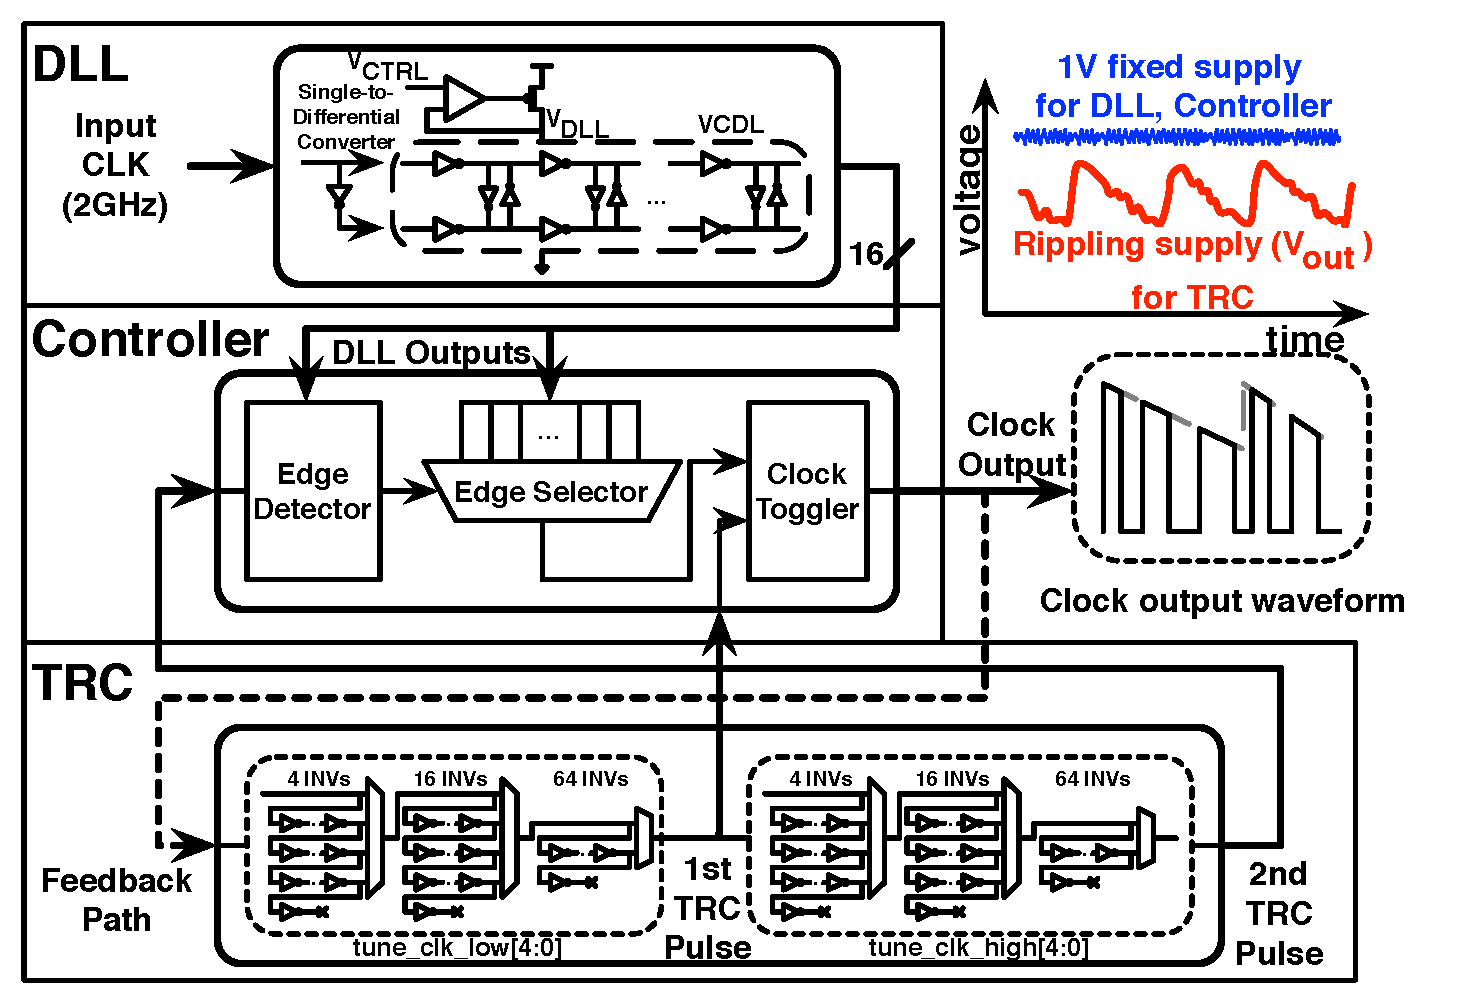
\includegraphics[width=0.6\textwidth]{clockgen-block}
  \caption{A block diagram of the DLL-based adaptive clock generator~\cite{Zimmer2016} ({\textcopyright} 2016 IEEE, reprinted with permission).}
  \label{fig:clockgen-block}
\end{figure}

The DLL contains voltage-controlled delay line (VCDL), the phase detector (PD), and the charge pump (CP) with the loop filter (LF).
The VCDL converts a single-ended global 2 GHz clock signal into 8 differential signals of the same frequency.
The single-ended input is converted to a differential pair by using an inverter, followed by cross-coupled differential inverter chains.
The cross-coupled differential delay unit is composed of two inverters for the main path, and two small inverters that connect the outputs of the main inverters to minimize the phase mismatch between the output nodes.

%The small coupling inverters are a quarter of the size of the main path inverters so as not to distort the signal on the path. To achieve better DLL outputs, the same differential units are used before and after the VCDL as a pre-buffer and a dummy load, respectively. The VCDL generates 16 phase references that have the same interval of 31.25 ps (500 ps/16), where the 16th phase matches the 0th phase. The delay line is designed to have the delay between the 0th reference and the 16th reference to be around 375 ps (75\% of 500 ps) at the nominal voltage of 1 V, so that the rising edge of the 16th reference can be initially located in the low period (between the falling edge and the next rising edge) of the 0th reference. This initial difference must be guaranteed for the correct operation of the DLL. The VCDL is controlled by a low-dropout (LDO) regulator which is composed of a CML- type differential amplifier and a large PMOS cell as a power gate. A large decoupling capacitor is connected to the power node of the VCDL to alleviate the voltage ripple due to logic switching. Since the output voltage level of the VCDL, which is controlled by the local LDO, is usually lower than a nominal voltage (1 V), a level shifter is added to each output signal. The level shifter is followed by a large buffer to minimize interval mismatch between adjacent outputs of the VCDL due to load mismatches.

%The phase detector compares the 0th phase and the 16th phase of the reference signals.
%The detector is composed of two phase detector units which are used to generate the UP and DN signals respectively, by connecting the appropriate phases to the inputs as shown in Fig. 12. The output F is initially zero. UP is asserted when the VCDL needs to be sped up, and DN is asserted when the VCDL needs to be slowed down. In the detector unit, the output F is set to ?1? only when the input B rises faster than the input A, and stays high until the input A is on. The pulse width of the output F is a function of the time difference between the two rising edges. For the DN detector unit, the 16th reference is connected to the input B and the 0th reference is connected to the input A. Similarly, the 0th reference is connected to the input B and the 16th reference is connected to the input A for the UP detector unit. At initialization, the 16th reference has its rising edge when the 0th reference is low, and so the phase detector detects that that the 16th reference has risen faster than the 0th reference and signals the charge pump to slow the VCDL by asserting DN.
%The charge pump determines the reference voltage level of the LDO. Using the UP and DN signals from the phase detector, this block charges or discharges the output node. The 500 fF of capacitance is placed at the output of the CP as a loop filter. To match the speed of charging and discharging, the transistor sizes of the PMOS and the NMOS are carefully
%selected. It also has a reset signal (EN), which forces the output to 1 V immediately as shown in Fig. 13.

The tunable replica circuit shown is placed in the processor core that is adaptively clocked.
The TRC is designed as a configurable inverter chain, and has two units that are independently controlled to set the duty cycle of the output clock.
Each unit consists of 124 identical inverter cells with a 5-bit control signal.
The configuration resolution is 4 FO1 delays, where FO1 is the fanout-of-one inverter delay.
Four inverter cells compose the resolution step, and the control signal determines how many resolution steps are used in the delay path.
%Since the number of inputs increases the mux delay exponentially, the delay path is divided into three stages, with two 4:1 muxes and a 2:1 mux.
%The first stage mux selects 0, 4, 8, or 12 inverter cells, the second stage mux selects 0, 16, 32, or 48 inverter cells, and the last mux selects 0 or 64 inverter cells.
%The minimum delay length is 0 inverters with 3 muxes when the control signal is ?00000,? while the maximum delay length is 124 inverters (12 from the first, 48 from the second, and the 64 from the last stage) with 3 muxes when the control signal is ?11111.?
The first unit sets the high phase of the clock, which starts at the rising edge and generates the falling edge, while the second unit is for the low phase.
With this feature, the period and the duty cycle can be independently adjusted.
%Two TRC units of 5-bit control each are equivalent of 6-bit control delay chains, resulting in a very wide tuning range of 0 to 248 FO1 inverter delays.
The TRC inverters are connected to the processor supply (VPROC) in order to track the critical path under voltage variations, while other logic remains in an isolated 1 V domain (V1V).
Therefore, 4 FO1 resolution is guaranteed at any supply voltage level, while the total delay is self-adjusted as a function of the supply.
TRC resolution is related to the phase resolution of the DLL.
TRC resolution finer than 4 FO1 would eventually be quantized by the DLL with the resolution of 31.25 ps, and will be ignored after passing the quantizer.
In the particular implementation, the 4 FO1 is about 25 ps at 1 V.

At the top level, the output clock signal is connected to the TRC input.
Two TRC units delay the rising edge of the input successively by the estimated critical path of the processor through appropriate digital calibration of the number of delay stages, and convert the delayed edges to pulses of short duration for the controller by using the pulse generators (PG).
The level shifters are located between the TRC and the PG, because the TRC units are on the processor?s voltage domain while the PG and the controller operate at 1 V.
The TRC goes into sleep mode to reduce the energy consumption when not in use by de-asserting the enable signal (EN).
Since the TRC delay directly determines the next clock period without any additional logic, the circuit achieves a response time of a single cycle.

The controller is composed of an edge detector, an edge selector, and a clock flip-flop.
The DLL references and the TRC pulses are the inputs to this block.
The clock output signal (CPOUT) is generated from the flip-flop followed by a large clock buffer.
The flip-flop data input is connected to VDD, its asynchronous reset input is connected to the first TRC output pulse (TP1), and its clock input (CI) is supplied by the edge selector.
%The first TRC output pulse asynchronously resets the flip-flop to generate the falling edge of the clock output.
%The second TRC output pulse (TP2), however, is not directly used to generate the rising edge because the rising edge should be synchronized to the DLL references.
%In the edge detector, the second TRC output pulse samples the DLL references to detect a reference phase that is about to rise.
%Since the reference signals have equivalent intervals, the sampled values(D0?D15) are eight continuing 0?s and eight continuing 1?s circularly, and the first 0 after the sequence of 1?s corresponds to the phase of upcoming rising edge.
%Each sampled signal is reset to zero by the DLL reference which is 4 phases ahead of the input (Pn?4).
%The edge selector picks the correct reference phase by using the result from the previous stage (Sn).
%The dynamic mux gate is used to speed up the operation.
%The gate is in evaluation phase only when the second TRC output pulse is high, and transitions to precharge phase when the pulse from the TRC is low.
%The mux output, which is a pulse, triggers the flip-flop as a clock signal.
%The entire waveform is represented in Fig. 16.

Since the DLL references and the TRC output pulse are asynchronous, the flip-flops in the edge detector may occasionally fail to sample the inputs, resulting in metastability.
%In Fig. 16, TP2 fails to sample Pn if two edges are close, and the output Dn does not settle on time.
%After passing several logic gates, the metastable signal is usually resolved to the stable logic level.
%If the Dn is settled to the incorrect value, Sn+1 is asserted instead of Sn, and CPOUT rises late by one DLL delay which is 31.25 ps.
%In most cases, the metastable outputs are resolved to ?0? or ?1? in a short time, so the entire operation remains correct.
%However, the control logic can malfunction if the selection signal, Sn, remains metastable, and thus the edge selector fails to generate the pulse CI.
%Without enough width of CI, the clock output signal is eventually set to zero, and may remain low.
To avoid this, a watchdog block is implemented.
This logic continuously monitors the status of the clock output signal, and generates an extra pulse for the clock flip-flop input when the clock output signal remains zero for longer than two clock delays of the previous period.
The clock output (CLKOUT) is synchronized to the global 2 GHz clock (CLKREF) which is also used in the DLL.
The sampled clock output is connected to the gate logic which generates the pulse, PU, that is asserted for a cycle when the sampled clock output goes high.
The free running counter is reset when PU is asserted, and sends the value to the reference.
If the clock output is metastable, the counter value exceeds the previous counter value stored in the reference without the PU assertion.
Although two clock signals are asynchronous, it is possible to estimate the clock skew because the CLKOUT is quantized by the DLL outputs which originated from CLKREF.
In the design phase, the skew is adjusted to minimize metastablility.

The clock generator is designed to conform to standard cell design rules to enable tight integration with the core logic.
By using same design style, and thus by embedding the block directly in the processor, the core and the clock generator can share operating conditions such as voltage and temperature.
The signal paths for the DLL references are manually routed, and the wire lengths are carefully matched to minimize any possible discrepancy in the delay intervals. The signal paths in the controller are routed in the same manner.
The watchdog is synthesized and automatically placed and routed.

\subsection{Free-running Adaptive Clocking}

A block diagram of the clock generator circuit implemented in Raven-4 is shown in Figure~\ref{fig:3-clockgen}~\cite{Keller2017}.
The adaptive clock generator is free-running and does not require any external reference.
The circuit generates clock edges via a D flip-flop, which is set or reset with pulse generators to toggle between one and zero.
After a rising clock edge is generated, the edge propagates through the first delay unit and then triggers a reset pulse on the flip-flop, causing the output to fall.
This edge then continues through the second delay unit and triggers a clock pulse on the flip-flop, resulting in a rising edge at the output.
This design allows the duty cycle of the generated clock to be adjusted.

\begin{figure}
  \centering
  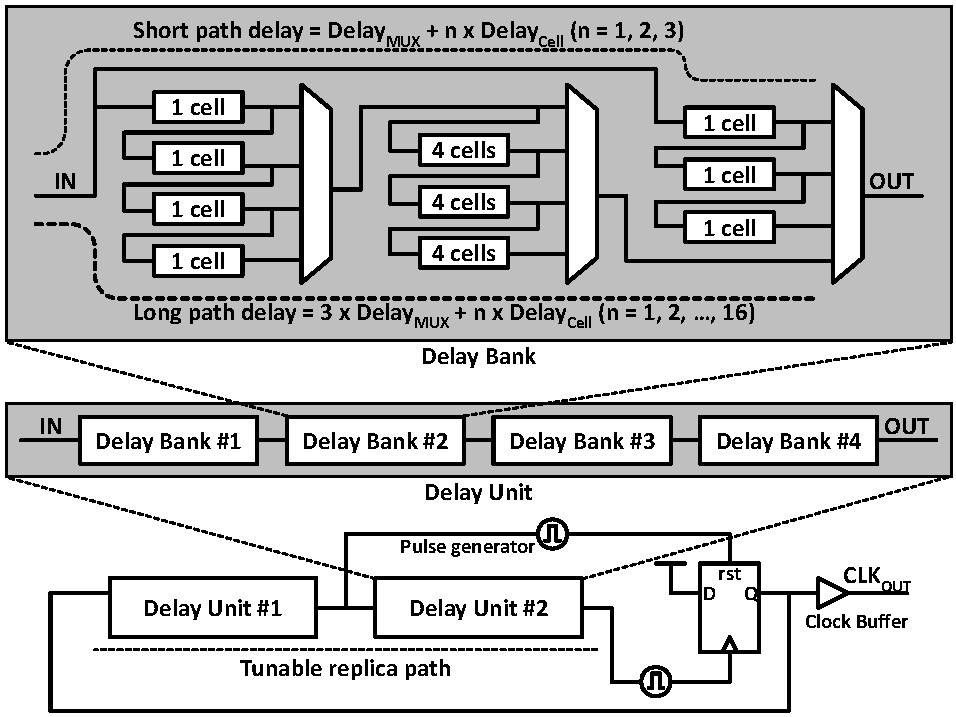
\includegraphics[width=0.8\textwidth]{3-clockgen}
  \caption{A block diagram of the free-running adaptive clock generator~\cite{Keller2017} ~\cite{Keller2016} ({\textcopyright} 2016 IEEE, reprinted with permission).}
  \label{fig:3-clockgen}
\end{figure}

The adaptive clock generator is supplied by the same rippling output voltage that is used to power the digital logic in the system.
The delay units therefore respond to voltage changes similarly to the digital logic; the propagation delays that trigger each clock edge face the same environment as the digital logic paths in the design.
Each delay unit is comprised of four delay banks, and each bank consists of a chain of a particular cell in addition to multiplexors and control logic that allow the number of cells in the delay chain to be selected.
The first bank uses a custom buffer cell design to balance rise and fall times.
Each of the remaining banks consists of a standard cell that was commonly observed in the synthesized critical paths of the digital logic.
Each bank uses a different combination of pMOS/nMOS ratio and gate length, as these characteristics affect the voltage-frequency relationship of the cells.
By selecting different mux settings, the delay paths can be tuned until they match the delay characteristics of the critical paths in the digital logic supplied by the generated clock, ensuring that the clock edges are generated at the appropriate frequency for the instantaneous voltage produced by the regulator.

\section{System Performance}

The Raven-3 and Raven-4 testchips were implemented in 28nm FD-SOI technology.
Measurement results demonstrate the effectiveness of the various systems implemented in the two testchips, showing the utility of FD-SOI technology in designing energy-efficient processor systems.
Table~\ref{tab:raven3-summary} shows a summary of the chip and key measurement results of the Raven-3 testchip, and Table~\ref{tab:raven4-summary} summarizes key features and measurement results of the Raven-4 testchip.

\begin{table}[]
\footnotesize
\renewcommand{\arraystretch}{1.2}
\centering
\begin{tabular}{@{}ll@{}}
\toprule
Technology & \SI{28}{\nano\meter} FDSOI\\ 
Die Area & \SI{1305}{\micro\meter} $\times$ \SI{1818}{\micro\meter} (\SI{2.37}{\milli\meter\squared})\\ 
Core Area & \SI{880}{\micro\meter} $\times$ \SI{1350}{\micro\meter} (\SI{1.19}{\milli\meter\squared})\\ 
Converter Area & 24 $\times$ \SI{90}{\micro\meter} $\times$ \SI{90}{\micro\meter} (\SI{0.19}{\milli\meter\squared})\\ 
Voltage & \SIrange{0.45}{1}{\volt} (1V FBB)\\ 
Frequency & \SIrange{93}{961}{\mega\hertz} (1V FBB) \\ 
Power & \SIrange{8}{173}{\milli\watt} (1V FBB)\\ 
SC density & \SI[per-mode=symbol]{11.0}{\femto\farad\per\micro\meter\squared}\\ 
SC power density &\SI[per-mode=symbol]{0.35}{\watt\per\milli\meter\squared} @ 88\% efficiency \\
\bottomrule
%\hline
\end{tabular}
\caption{A summary of key results and details from the Raven-3 testchip~\cite{Zimmer2016}.}
\label{tab:raven3-summary}
\end{table}

\begin{table}[]
\footnotesize
\renewcommand{\arraystretch}{1.2}
\centering
\begin{tabular}{@{}ll@{}}
\toprule
Technology & \SI{28}{\nano\meter} FDSOI\\
Die Area & \SI{1665}{\micro\meter} $\times$ \SI{1818}{\micro\meter} (\SI{3.03}{\milli\meter\squared})\\
Core Area & \SI{895}{\micro\meter} $\times$ \SI{1193}{\micro\meter} (\SI{1.07}{\milli\meter\squared})\\
Standard Cells & 568K \\
Converter Area & 48 $\times$ \SI{90}{\micro\meter} $\times$ \SI{90}{\micro\meter} (\SI{0.39}{\milli\meter\squared})\\
Core Voltage & \SIrange{0.48}{1}{\volt} (bypass mode)\\
Core Power & \SIrange{1.2}{231}{\milli\watt} (bypass mode)\\
Core Frequency & \SIrange{20}{797}{\mega\hertz} (bypass mode)\\
Peak Energy Efficiency & 41.8 GFLOPS/W (1/2 1V mode)\\
Conversion Efficiency & 82-89\%\\
AVS Transition Time & $<$\SI{1}{\micro\second}\\
Peak AVS Energy Savings & 39.8\%\\
\bottomrule
\end{tabular}
\caption{A summary of key results and details from the Raven-4 testchip~\cite{Keller2017}.}
\label{tab:raven4-summary}
\end{table}


\subsection{Raven-3 Measurement Results}

%The Raven-3 testchip was wirebonded directly to a daughterboard to minimize bond wire inductance.
%A multimeter or oscilloscope connects to sense points on the daughterboard to measure the output voltage rail supplied by the SS-SC converter.
%The daughterboard is connected via an FPGA Mezzanine Card (FMC) connector to a motherboard which generates the necessary clocks, supplies, and reference voltages.
%Additional testpoints on the motherboard connect to a sourcemeter to measure the input power provided to the SS-SC converter.
%The motherboard connects via a second FMC to a ZedBoard~\cite{ZedBoard} that includes an FPGA and a network-accessible ARM core.
%The serialized 16-bit digital interface of the testchip is connected to programmable logic in the FPGA, which can route memory traffic to local DRAM and emulate system calls.
%Software running on the ARM core acts as a host controller for the tethered test chip processor.
%Figure~\ref{fig:6-raven3-test-setup-diagram} shows a block diagram of the test setup, and Figure~\ref{fig:6-raven3-test-setup} shows a photograph of the system configured for test.

%\begin{figure}
%  \centering
%  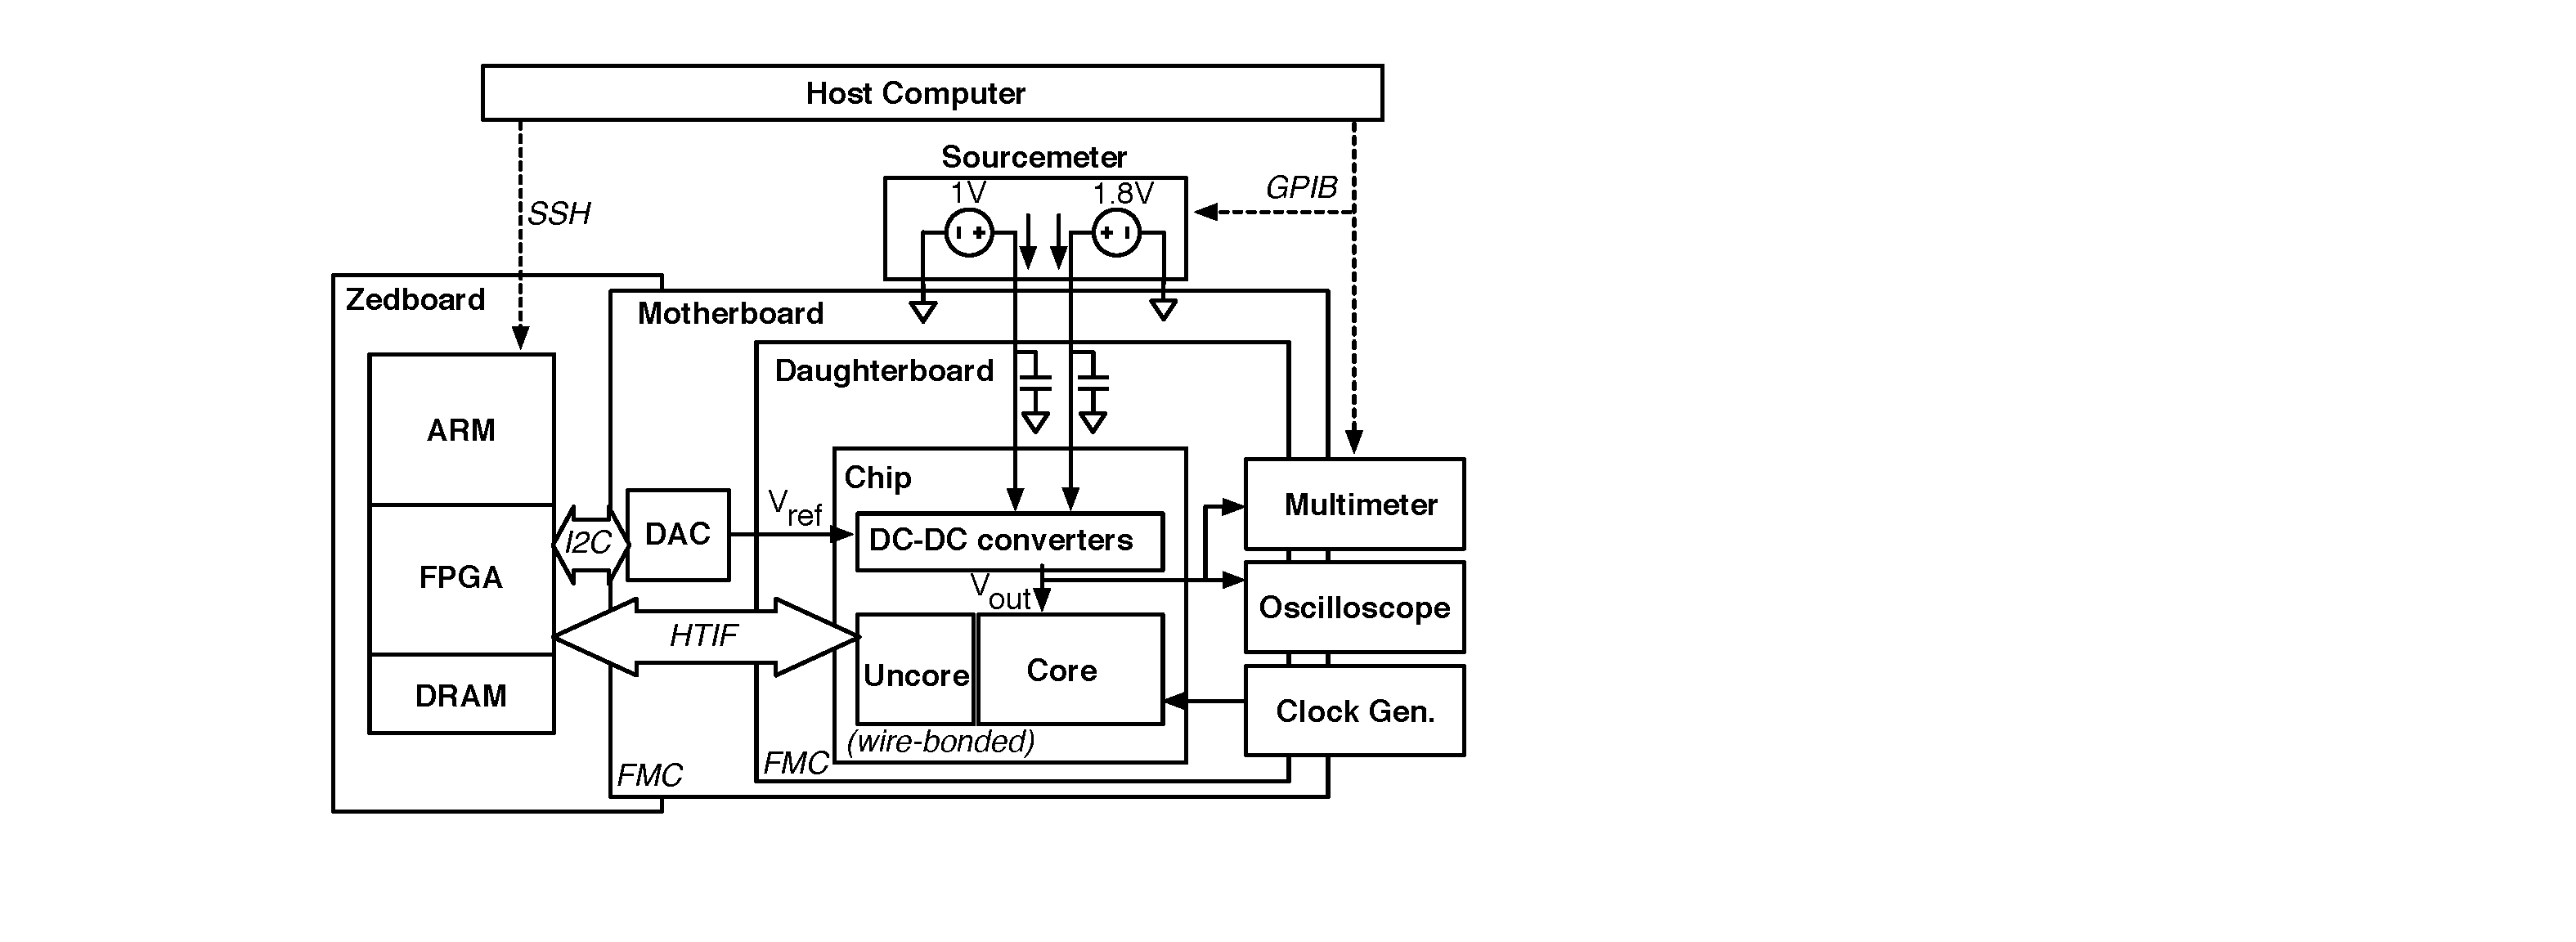
\includegraphics[width=0.8\textwidth]{6-raven3-test-setup-diagram}
%  \caption{A block diagram showing the test setup of the Raven-3 testchip~\cite{Zimmer2016} ({\textcopyright} 2016 IEEE).}
%  \label{fig:6-raven3-test-setup-diagram}
%\end{figure}
%
%\begin{figure}
%  \centering
%  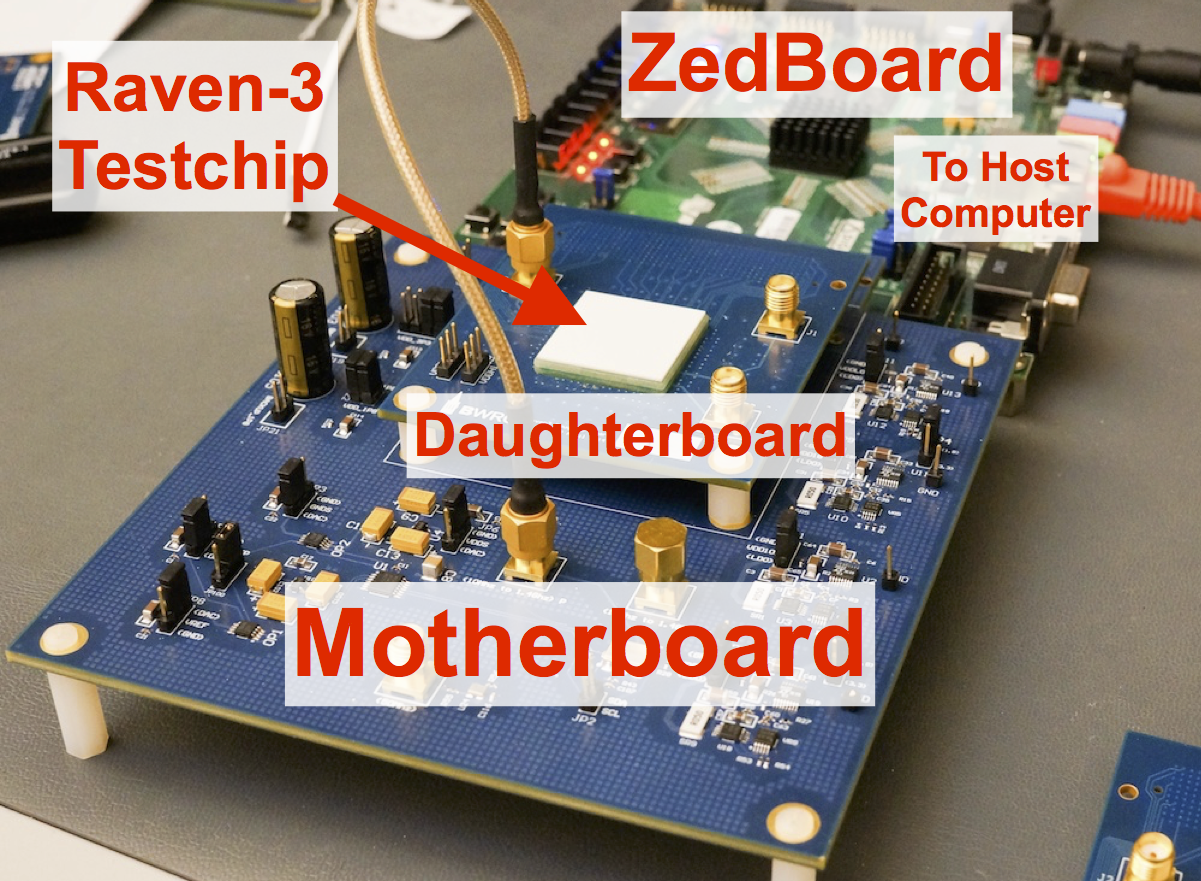
\includegraphics[width=0.7\textwidth]{6-raven3-test-setup}
%  \caption{The Raven-3 testchip and associated infrastructure.  The chip itself is obscured by the white protective covering.}
%  \label{fig:6-raven3-test-setup}
%\end{figure}
%
Figure~\ref{fig:6-raven3-dcdc-waveforms} shows oscilloscope traces of the rippling core voltage domain for all four SS-SC regulator configurations.
As noted in Section~\ref{sec:sc-dcdc}, simultaneous-switching converters do not completely eliminate charge sharing because the load itself has a capacitive component.
This results in observed average output voltages that are lower than the ideal ratios.
Figure~\ref{fig:6-raven3-dcdc-ref} shows the impact of adjusting the lower-bound reference voltage $V_{ref}$ on conversion efficiency.
Changing the reference voltage changes both the average output voltage and the switching rate of the converter, which affects the conversion efficiency.
Each switching mode has a particular $V_{ref}$ that achieves maximum efficiency at a given load.
Different processor loads correspond to different optimal $V_{ref}$ because the processor load affects the switching frequency of the regulators.

\begin{figure}
  \centering
  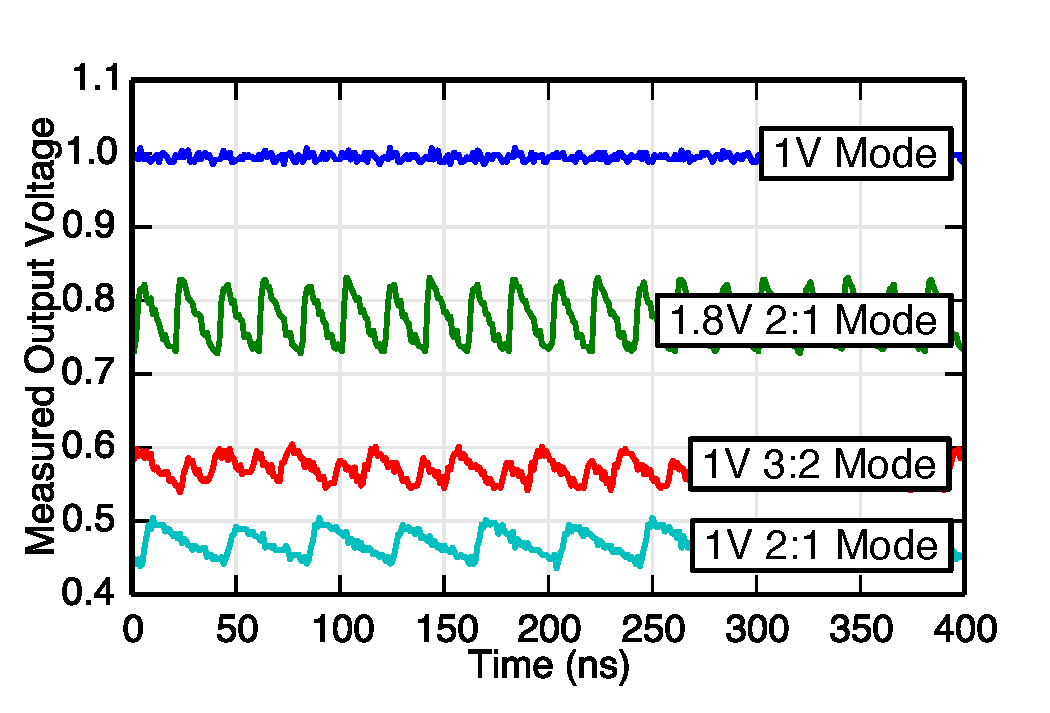
\includegraphics[width=0.6\textwidth]{6-raven3-dcdc-waveforms}
  \caption{Oscilloscope traces of the voltages generated in the four SS-SC operating modes~\cite{Zimmer2016} ({\textcopyright} 2016 IEEE, reprinted with permission).}
  \label{fig:6-raven3-dcdc-waveforms}
\end{figure}

\begin{figure}
  \centering
  \hspace*{\fill}
  \begin{subfigure}[t]{0.45\textwidth}
  \centering
  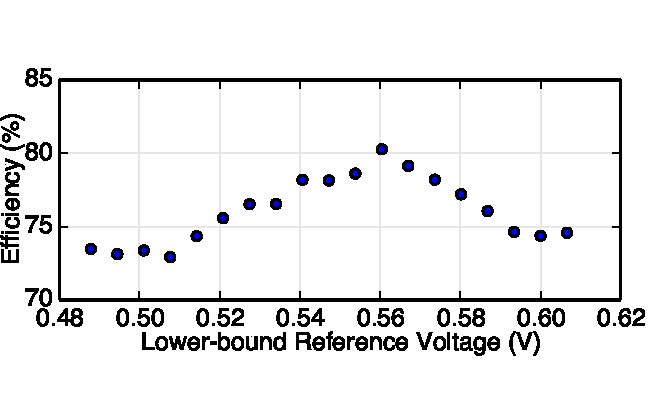
\includegraphics[width=\textwidth]{6-raven3-dcdc-ref-a}
  \caption{}
  \label{fig:6-raven3-dcdc-ref-a}
  \end{subfigure}
  \hspace*{\fill}
  \begin{subfigure}[t]{0.45\textwidth}
  \centering
  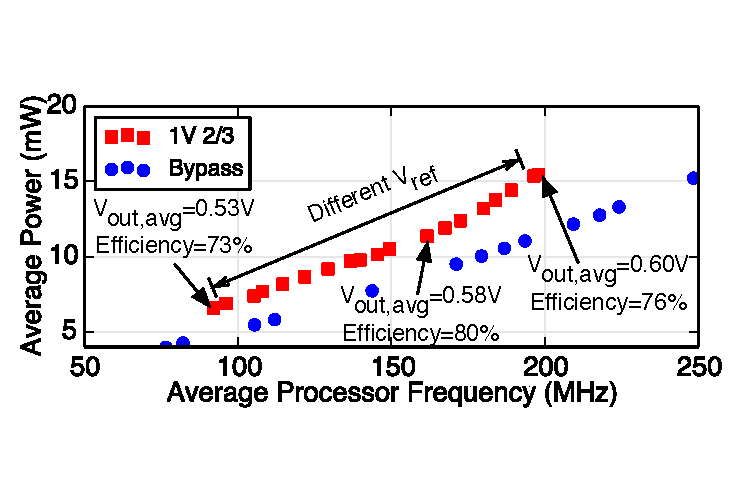
\includegraphics[width=\textwidth]{6-raven3-dcdc-ref-b}
  \caption{}
  \label{fig:6-raven3-dcdc-ref-b}
  \end{subfigure}
  \hspace*{\fill}
  \caption{Figures showing the effect of different lower-bound reference voltages on system operation~\cite{Zimmer2016} ({\textcopyright} 2016 IEEE, reprinted with permission).  (\subref{fig:6-raven3-dcdc-ref-a}) shows the system conversion efficiency as the voltage is swept, and (\subref{fig:6-raven3-dcdc-ref-b}) shows the effect of different $V_{ref}$ on average output voltage and frequency.}
  \label{fig:6-raven3-dcdc-ref}
\end{figure}

For all possible converter topologies with adaptive clocking, the processor successfully boots Linux and runs user applications, demonstrating that complex digital logic operates reliably with an intentionally rippling supply voltage.
Figure~\ref{fig:6-raven3-dcdc-modes} shows the rapid ($<$\SI{20}{\nano\second}) transitions between different voltage modes.
The application core can continue to operate through these mode transitions, demonstrating the utility of integrated regulators for FG-AVS.

\begin{figure}
  \centering
  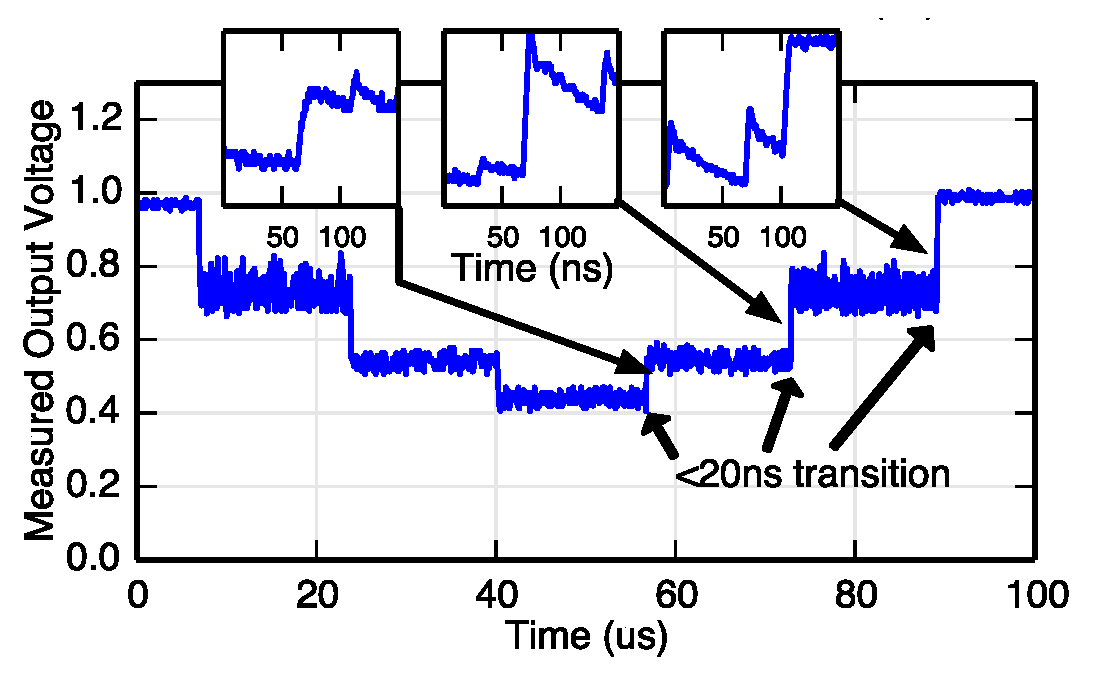
\includegraphics[width=0.6\textwidth]{6-raven3-dcdc-modes}
  \caption{An oscilloscope trace showing the generated core voltage as the SS-SC converter rapidly cycles through each of the four operating modes~\cite{Zimmer2016} ({\textcopyright} 2016 IEEE, reprinted with permission).}
  \label{fig:6-raven3-dcdc-modes}
\end{figure}

%The conversion efficiency of voltage converters is generally computed by measuring the current and voltage on both the input and output of the converter to measure the ratio of power delivered to power supplied.
%The regulator in the Raven-3 testchip cannot be measured in this way because it is it is difficult to measure on-chip voltage and current since the voltage is rippling very quickly.
%Furthermore, even if power output of the converter could be measured, this metric would ignore the impact of imperfect adaptive clock tracking, which is an important loss component.
%Therefore, a different method is required to measure the efficiency of the implemented system.

System conversion efficiency measurements include all sources of overhead, including non-idealities in the adaptive clock.
As shown in Figure~\ref{fig:6-raven3-dcdc-efficiency}, the measured voltage conversion efficiency ranges from 80\% to 86\% for the different output voltage modes.

\begin{figure}
  \centering
  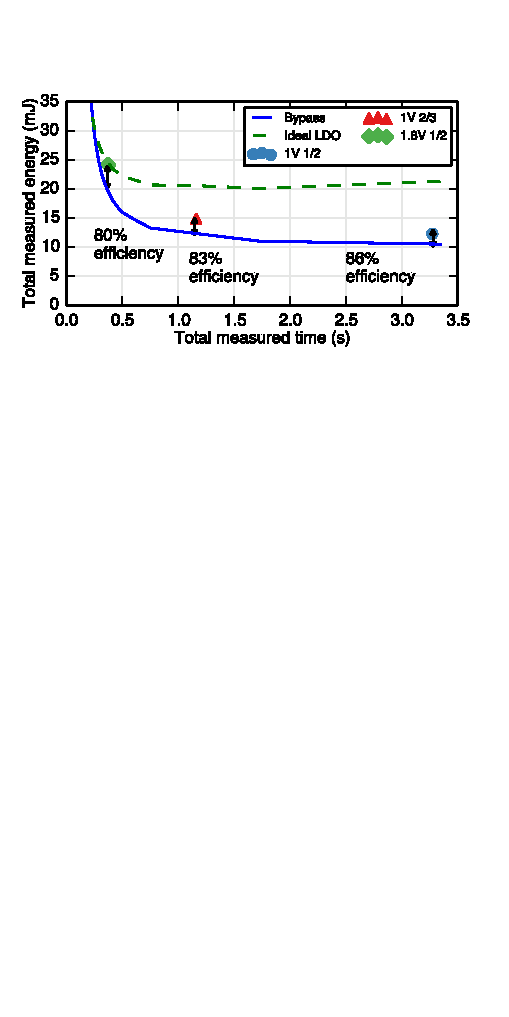
\includegraphics[width=0.65\textwidth]{6-raven3-dcdc-efficiency}
  \caption{A plot demonstrating the system conversion efficiency of the three SS-SC switching modes~\cite{Zimmer2016} ({\textcopyright} 2016 IEEE, reprinted with permission).}
  \label{fig:6-raven3-dcdc-efficiency}
\end{figure}

%We define system conversion efficiency as the ratio of energy required to finish the same workload in the same amount of time under the regulated system as compared to a system without voltage conversion losses.
%In this metric, 100\% efficiency represents a lossless regulator supplying the core as it operates at the maximum frequency achievable at that voltage.
%To determine this 100\%-efficiency baseline, the bypass mode is used to directly supply the core with an ideal off-chip voltage source.
%A self-checking benchmark is run for a fixed number of cycles at different voltages, and a binary search is performed at each voltage point to find the maximum frequency.
%At the maximum frequency, the total elapsed time and total energy to run the fixed-length benchmark is measured, where the energy is computed by measuring the current drawn from the off-chip supply and the delivered voltage is measured from sense points on the core voltage (to remove the voltage drop across the on-chip bypass-mode power gates from the efficiency calculation).
%This baseline provides the blue curve in the Figure~\ref{fig:6-raven3-dcdc-efficiency} and represents a 100\%-efficient off-chip regulator.
%Then, for each SS-SC mode, the same benchmark is run for the same number of cycles, and the total elapsed time and energy is measured.
%Due to non-idealities of the converter, it takes more energy to perform the same task in the same amount of time.
%Therefore, system conversion efficiency is defined as the ratio of energy required to finish the same workload in the same time.

\begin{figure}
  \centering
  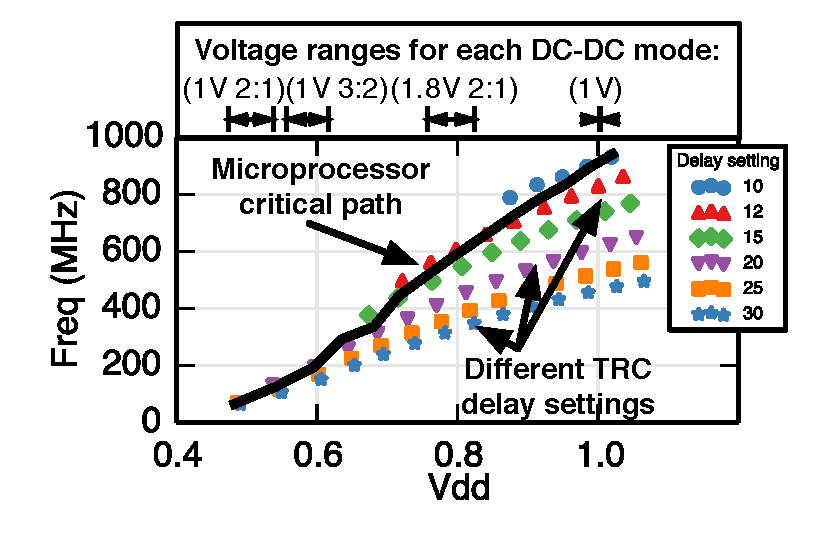
\includegraphics[width=0.55\textwidth]{6-raven3-clock}
  \caption{Measurements of the adaptive clock generator frequency over different voltages and replica path delay settings~\cite{Zimmer2016} ({\textcopyright} 2016 IEEE, reprinted with permission). }
  \label{fig:6-raven3-clock}
\end{figure}

Figure~\ref{fig:6-raven3-clock} shows measured average frequency for different delay settings for the tunable replica circuit across a range of operating voltages (supplied using the bypass mode).
Annotations above the plot indicate the approximate voltage ranges seen in each SS-SC voltage mode.
Because the inverter-based replica path delay characteristics do not match the critical paths of the processor, a single delay setting poorly tracks the processor critical path over the entire voltage range.
At higher voltages, a shorter replica path delay best tracks the processor critical path, while at lower voltages, a longer replica path delay best tracks the processor critical path.
However, manual calibration of specific delay settings for each SS-SC voltage mode allows reasonably accurate tracking within the relatively small ripple of that mode.

\begin{figure}
  \centering
  \hspace*{\fill}
  \begin{subfigure}[t]{0.23\textwidth}
  \centering
  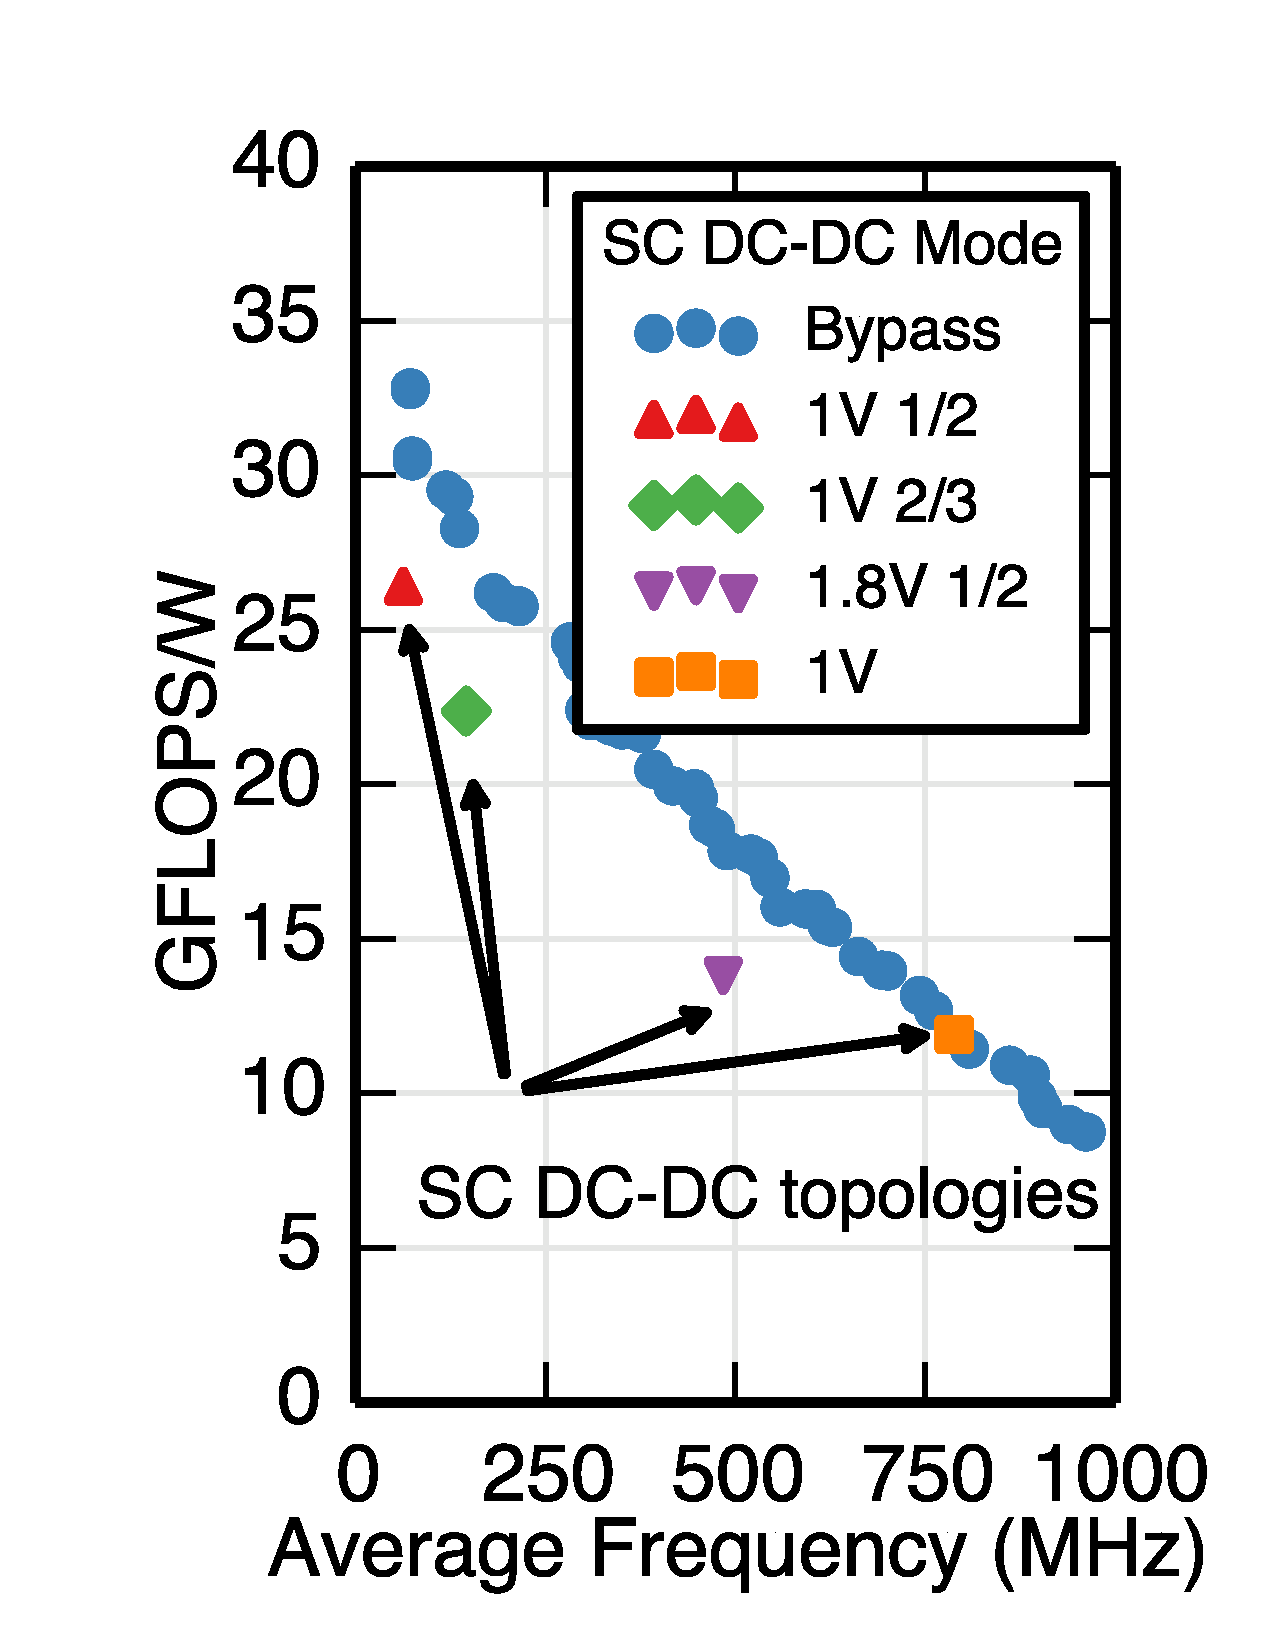
\includegraphics[width=\textwidth]{6-raven3-shmoo-a}
  \caption{}
  \label{fig:6-raven3-shmoo-a}
  \end{subfigure}
  \hspace*{\fill}
  \begin{subfigure}[t]{0.23\textwidth}
  \centering
  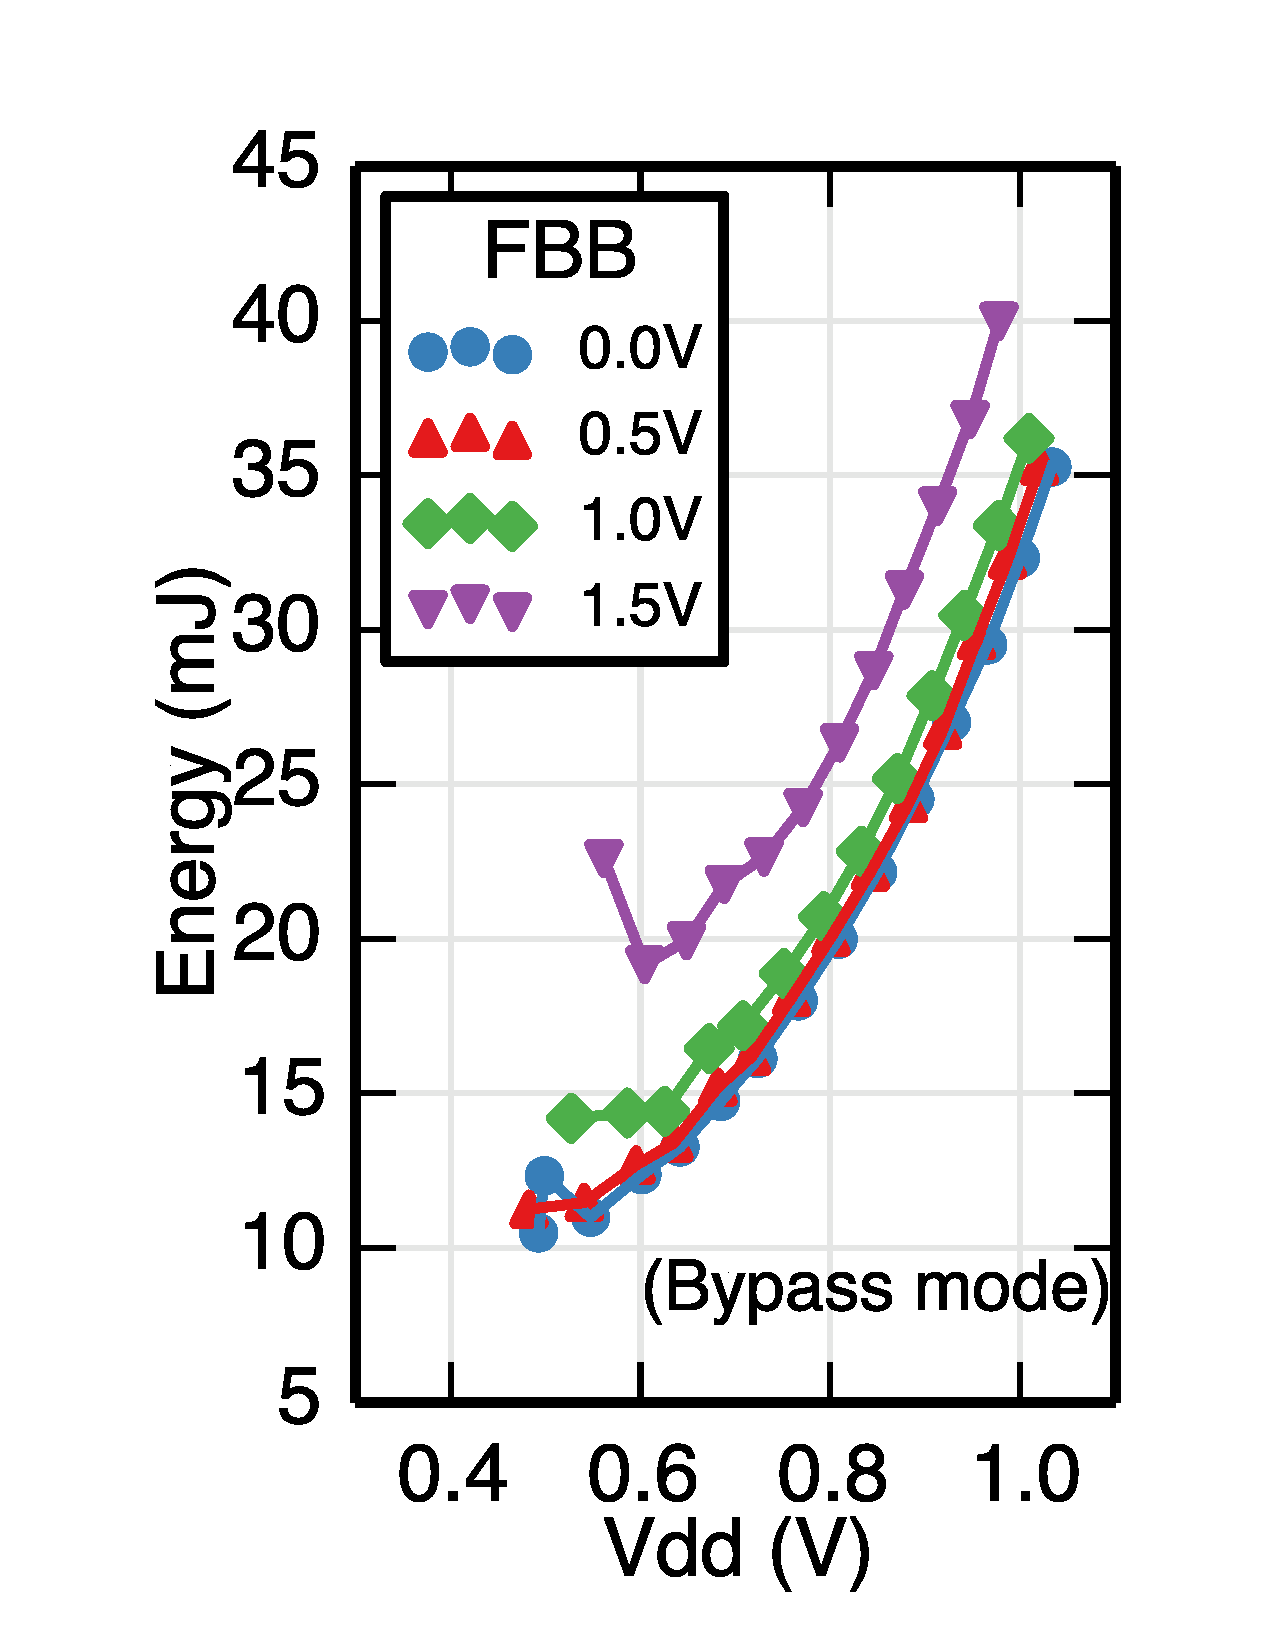
\includegraphics[width=\textwidth]{6-raven3-shmoo-b}
  \caption{}
  \label{fig:6-raven3-shmoo-b}
  \end{subfigure}
  \hspace*{\fill}
  \begin{subfigure}[t]{0.23\textwidth}
  \centering
  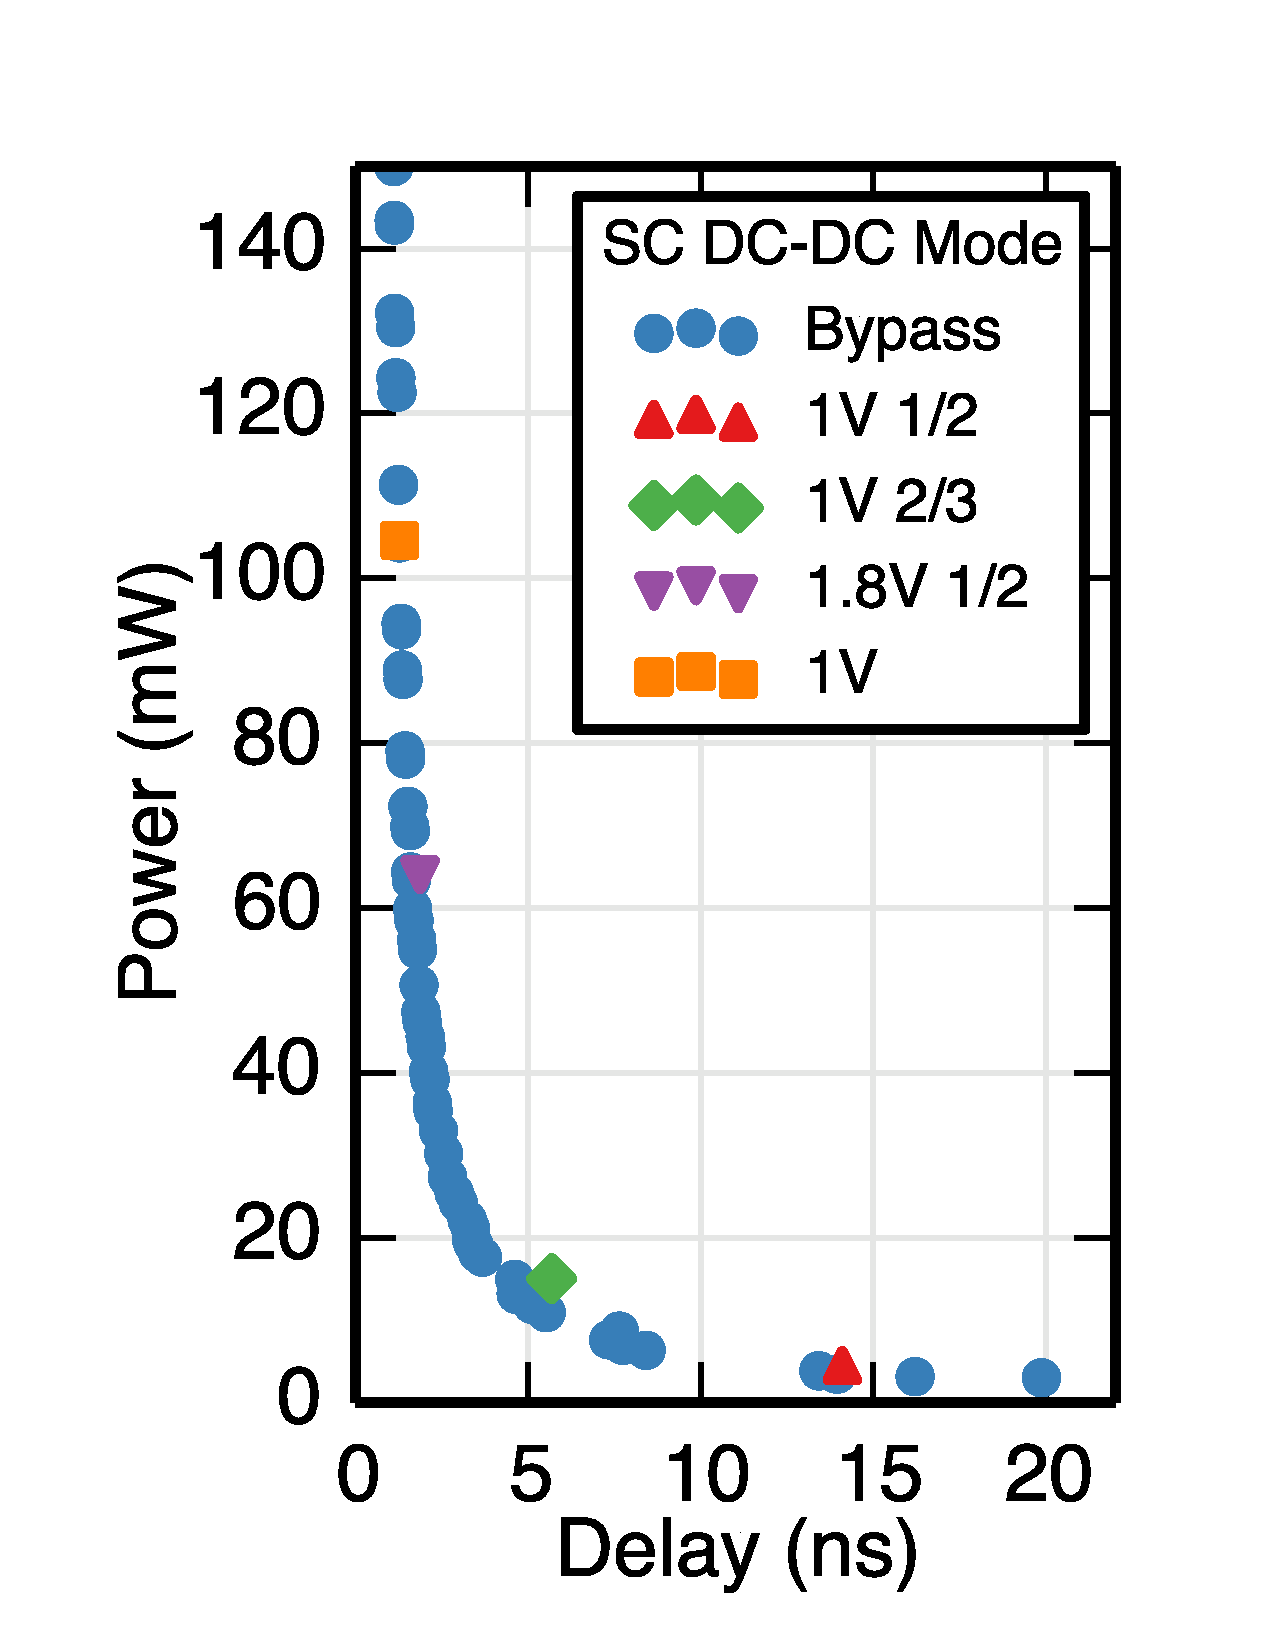
\includegraphics[width=\textwidth]{6-raven3-shmoo-c}
  \caption{}
  \label{fig:6-raven3-shmoo-c}
  \end{subfigure}
  \hspace*{\fill}
  \begin{subfigure}[t]{0.23\textwidth}
  \centering
  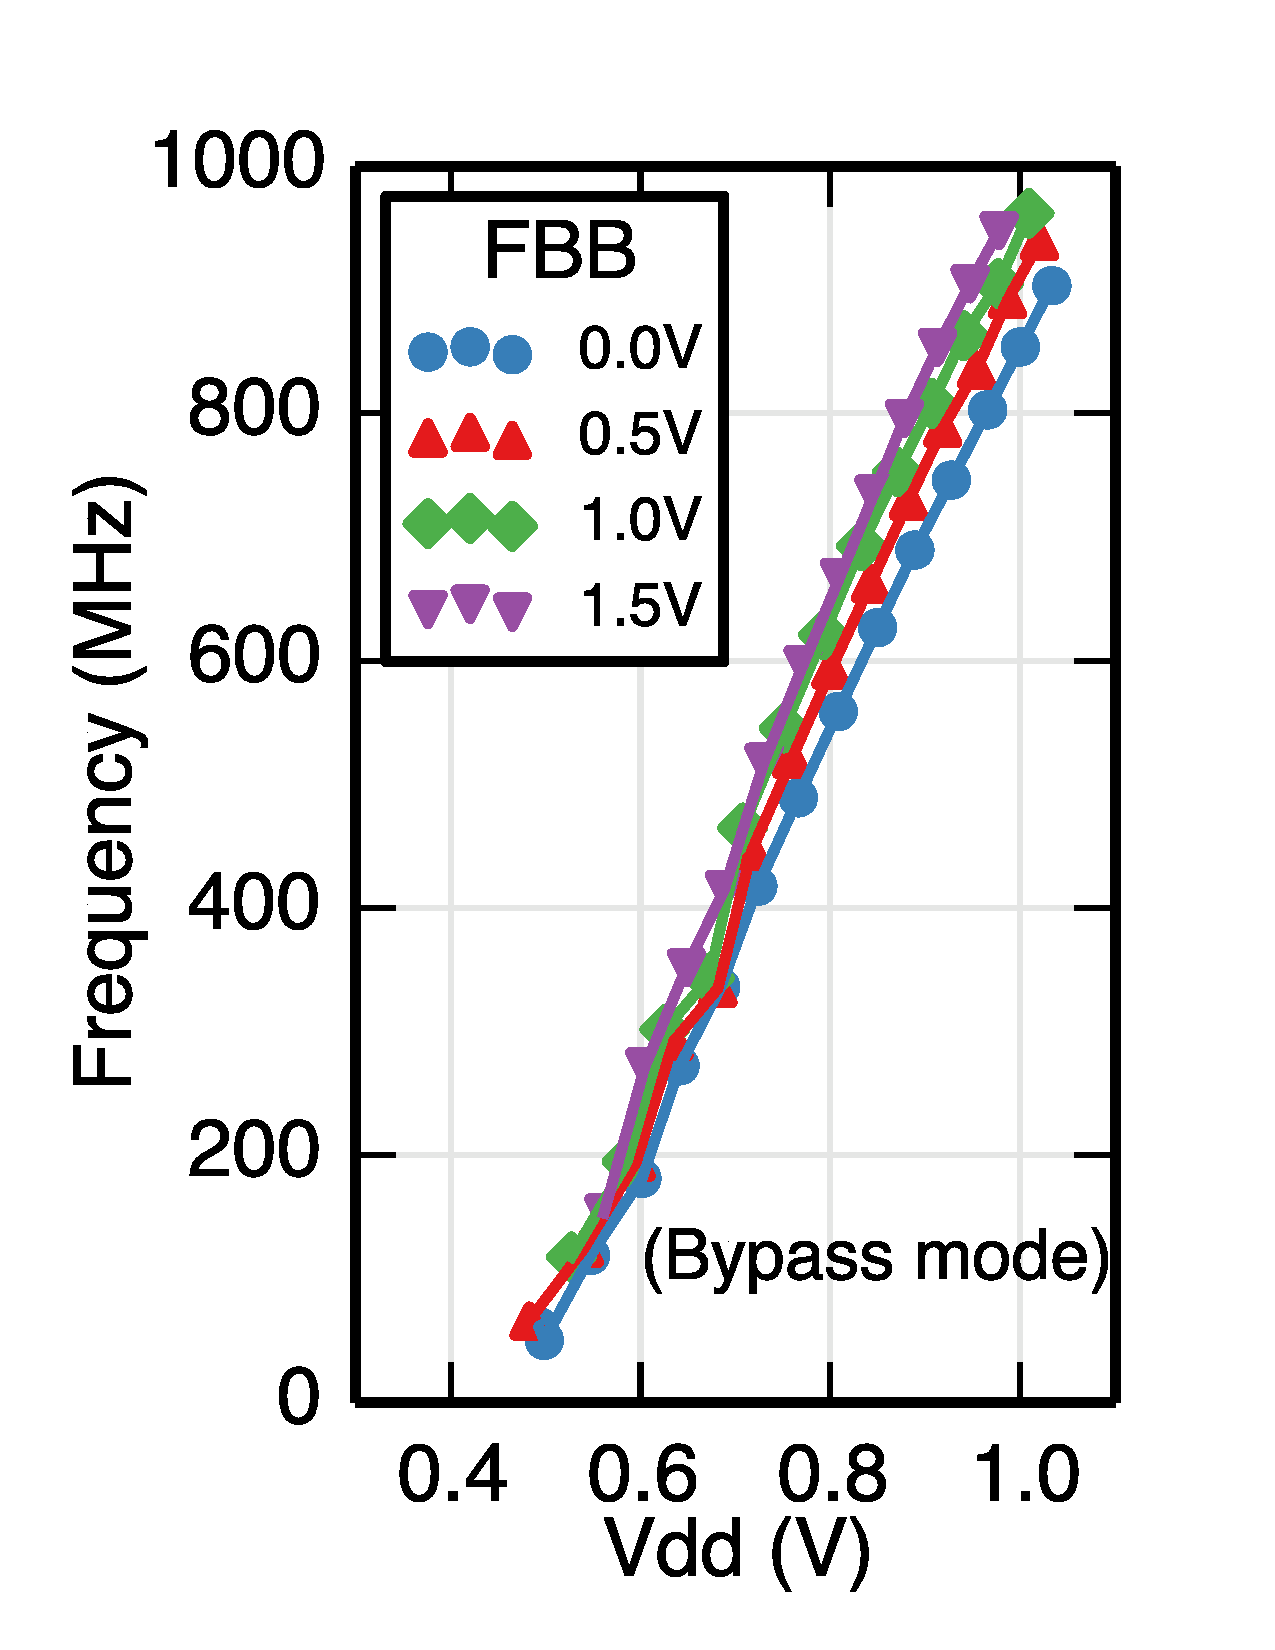
\includegraphics[width=\textwidth]{6-raven3-shmoo-d}
  \caption{}
  \label{fig:6-raven3-shmoo-d}
  \end{subfigure}
  \hspace*{\fill}
  \caption{Plots showing the measured energy, power, and frequency of the processor core in bypass mode and with the switching regulators enabled~\cite{Zimmer2016} ({\textcopyright} 2016 IEEE, reprinted with permission).}
  \label{fig:6-raven3-shmoo}
\end{figure}

Figure~\ref{fig:6-raven3-shmoo} shows various energy-delay curves for the application processor.
Energy efficiency is measured by measuring total core energy consumption while executing a fixed-length double-precision floating-point matrix multiplication kernel on the vector accelerator, and is shown both under bypass mode and when accounting for the losses of the switching regulation modes.
By using the on-chip converter to generate the lowest output voltage, the system achieves a peak efficiency of 26.2 GFLOPS/W.
The FD-SOI technology of the testchip enables up to \SI{1.8}{\volt} of FBB to be safely applied, which trades off improved performance for increased leakage~\cite{Jacquet2014}.
Figures~\ref{fig:6-raven3-shmoo-b} and \ref{fig:6-raven3-shmoo-d} show the impact of FBB on frequency and energy.
In each of the plots, each point represents the best achievable operating frequency at a given voltage.
The integrated system is able to achieve high energy efficiencies under the proposed voltage regulation and clocking scheme, demonstrating the potential utility of FG-AVS.

\subsection{Raven-4 Measurement Results}

%The Raven-4 testchip was wirebonded chip-on-board (see Figure~\ref{fig:6-raven4-wirebond}) and connected to an FPGA controller in a similar manner to Raven-3.

\begin{figure}
  \centering
  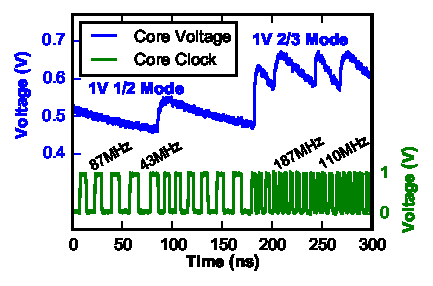
\includegraphics[width=0.5\textwidth]{6-raven4-waveforms}
  \caption{Oscilloscope traces of the core voltage and clock during an SS-SC mode transition~\cite{Keller2017} ~\cite{Keller2016} ({\textcopyright} 2016 IEEE, reprinted with permission).}
  \label{fig:6-raven4-waveforms}
\end{figure}

Figure~\ref{fig:6-raven4-waveforms} shows measured waveforms of the core voltage and core clock during a transition between voltage modes.
The core clock was measured via the output driver, which was not present on Raven-3.
The core clock adapts automatically to the voltage ripples within each mode and to the large voltage transition between modes.
Table~\ref{tab:raven4-efficiency} shows the peak system conversion efficiency of each of the three switching SS-SC modes.
The adaptive clock is tuned at each voltage setting by sweeping the settings of its replica delay path and choosing the fastest setting that still results in correct core functionality.
The adaptive clocking system provides a large improvement in system conversion efficiency because the core is able to operate at a higher average frequency as the supply voltage ripples, reducing the amount of energy required to complete the same amount of work.
When supplied by the SS-SC converter, the processor achieves a peak energy efficiency of 41.8 double-precision GFLOPS/W running an FMA microbenchmark on the vector coprocessor in 1/2 \SI{1}{\volt} mode.
The processor is able to boot Linux and run user programs while powered by the rippling supply voltage and adaptive clock.

\begin{table}[t]
\footnotesize
\renewcommand{\arraystretch}{1.2}
\centering
\begin{tabular}{@{}lll@{}}
\toprule
\textbf{DC-DC Mode} & \textbf{Efficiency (Adaptive Clock)} & \textbf{Efficiency (Fixed Clock)} \\
\midrule
1/2 1.8V & 88.7\% & 76.6\% \\
2/3 1.0V & 85.0\% & 75.4\% \\
1/2 1.0V & 81.6\% & 61.9\% \\
\bottomrule
\hline
\end{tabular}
\caption{Measured system conversion efficiencies achieved by the Raven-4 system~\cite{Keller2017}.}
\label{tab:raven4-efficiency}
\end{table}

\begin{figure}
  \centering
  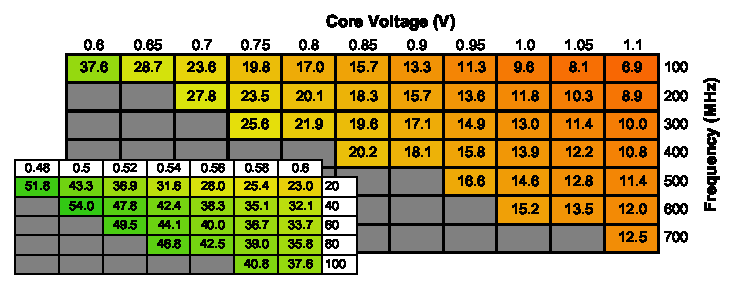
\includegraphics[width=0.8\textwidth]{6-raven4-shmoochart}
  \caption{A shmoo chart showing processor performance while executing a matrix-multiply benchmark under a wide range of operating modes~\cite{Keller2016} ({\textcopyright} 2016 IEEE, reprinted with permission). The number in each box represents the energy efficiency of the application core as measured in double-precision GFLOPS/W.}
  \label{fig:6-raven4-shmoochart}
\end{figure}

Figure~\ref{fig:6-raven4-shmoochart} shows the processor functionality across a wide range of voltages and frequencies.
The SS-SC converter is placed into bypass mode for characterization, allowing the measurement of processor performance under fixed voltage and frequency.
The best energy efficiency in bypass mode of 54.0 double-precision GFLOPS/W is achieved at \SI{500}{\milli\volt} and \SI{40}{\mega\hertz}.
Figure~\ref{fig:6-raven4-shmoo} shows the best frequency achievable at each operating point and the total energy consumed by a fixed-duration matrix-multiply benchmark at that operating point.
The application of FBB increases performance but results in higher leakage power.
The FBB voltage that achieves minimum energy depends on the proportion of switching power to leakage power and is therefore benchmark-dependent.
Figure~\ref{fig:6-raven4-fbb} shows that the energy of more computationally intensive benchmarks is minimized at higher body-bias settings.

\begin{figure}
  \centering
  \hspace*{\fill}
  \begin{subfigure}[t]{0.4\textwidth}
  \centering
  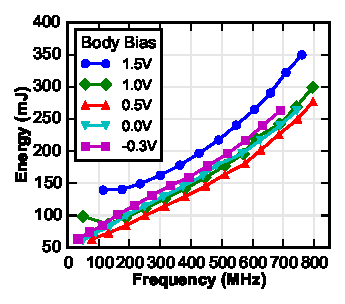
\includegraphics[width=\textwidth]{6-raven4-shmoo-a}
  \caption{}
  \label{fig:6-raven4-shmoo-a}
  \end{subfigure}
  \hspace*{\fill}
  \begin{subfigure}[t]{0.4\textwidth}
  \centering
  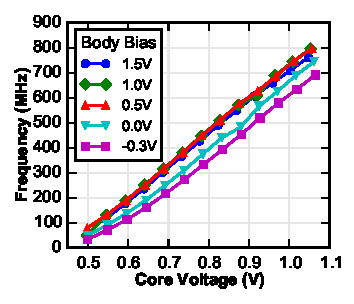
\includegraphics[width=\textwidth]{6-raven4-shmoo-b}
  \caption{}
  \label{fig:6-raven4-shmoo-b}
  \end{subfigure}
  \hspace*{\fill}
  \caption{Plots showing the effects of FBB on core frequency and energy~\cite{Keller2016} ({\textcopyright} 2016 IEEE, reprinted with permission).}
  \label{fig:6-raven4-shmoo}
\end{figure}

\begin{figure}
  \centering
  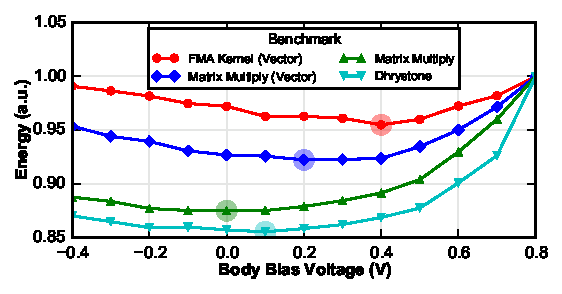
\includegraphics[width=0.7\textwidth]{6-raven4-fbb}
  \caption{The effect of FBB on different benchmarks with a supply voltage of 0.6V (bypass mode)~\cite{Keller2016} ({\textcopyright} 2016 IEEE, reprinted with permission).  The total energy consumed by each benchmark has been normalized so the relative effects of body bias can be compared.  The minimum-energy point is highlighted for each benchmark.}
  \label{fig:6-raven4-fbb}
\end{figure}

\begin{figure}
  \centering
  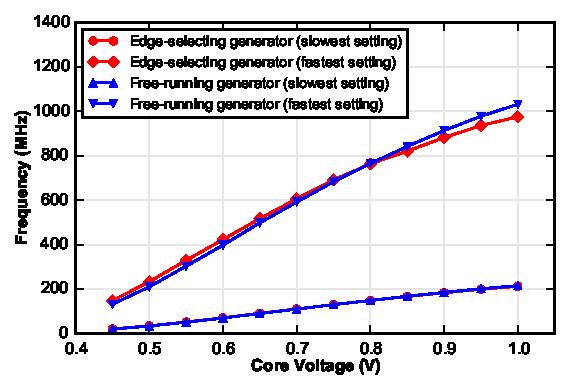
\includegraphics[width=0.7\textwidth]{6-raven4-clockgen}
  \caption{Measured comparison of the two clock generators implemented in the Raven-4 testchip~\cite{Keller2017} ({\textcopyright} 2017 IEEE, reprinted with permission).}
  \label{fig:6-raven4-clockgen}
\end{figure}

Figure~\ref{fig:6-raven4-clockgen} compares the generated frequency of the free-running adaptive clock generator with the design from Raven-3.
Both designs reliably generate a core clock that can supply the core area while a workload is executed on the application core.
The two designs track voltage similarly at the slowest delay settings, but the tracking varies at the fastest setting because the free-running design oscillates entirely in the variable-voltage domain, while part of the timing loop in the edge-selecting design is level-shifted to the fixed \SI{1}{\volt} supply.
The free-running generator achieves the same functionality as the adaptive clocking scheme from Raven-3 while simplifying the design and reducing area and power overhead.

\begin{figure}
  \centering
  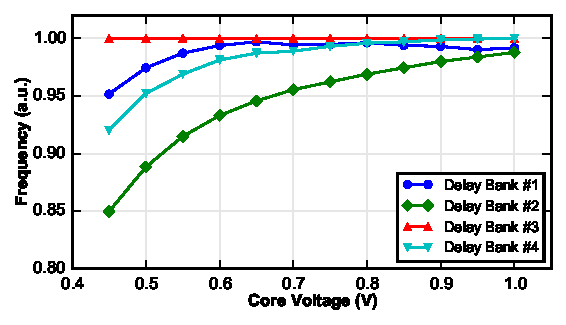
\includegraphics[width=0.7\textwidth]{6-raven4-clockgen-trc}
  \caption{Measurement results showing the relative difference in voltage-dependent frequency behavior of the four delay banks in the adaptive clock generator~\cite{Keller2017, reprinted with permission} ({\textcopyright} 2017 IEEE, reprinted with permission).}
  \label{fig:6-raven4-clockgen-trc}
\end{figure}

Figure~\ref{fig:6-raven4-clockgen-trc} compares the voltage-dependent delay characteristics of the four delay banks, normalized to the delay of the custom buffer cells in Bank 3.
The result for each bank was measured by recording the frequency of the generated clock after selecting the maximum delay through that bank and the minimum delay through the remaining banks.
The cells with small pMOS/nMOS ratios and larger gate lengths have larger delays at lower voltages.
The wide variation in voltage-dependent delays between the different delay banks (up to 18\% at \SI{0.45}{\volt}) validates the need for multiple different standard cells to achieve accurate critical path tracking.

\begin{figure}
  \centering
  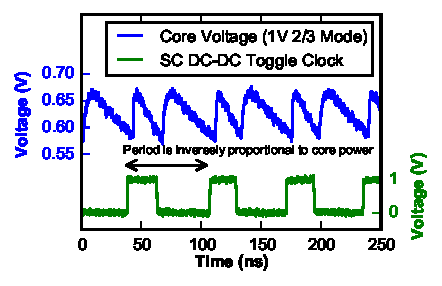
\includegraphics[width=0.5\textwidth]{6-raven4-waveforms-powermeas}
  \caption{Oscilloscope traces showing the rippling core supply voltage and the SS-SC toggle clock~\cite{Keller2016} ({\textcopyright} 2016 IEEE, reprinted with permission).}
  \label{fig:6-raven4-waveforms-powermeas}
\end{figure}

\begin{figure}
  \centering
  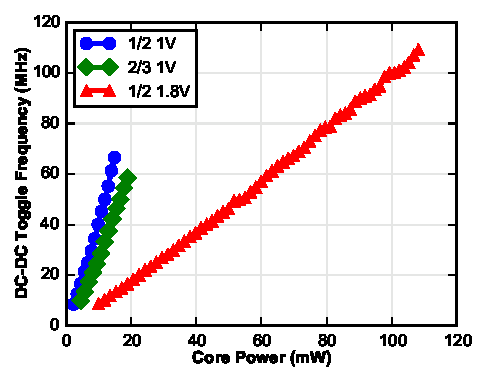
\includegraphics[width=0.6\textwidth]{6-raven4-powermeas}
  \caption{Measurement results showing the correlation between SS-SC toggle frequency and measured core power~\cite{Keller2017} ({\textcopyright} 2017 IEEE, reprinted with permission).}
  \label{fig:6-raven4-powermeas}
\end{figure}

Figure~\ref{fig:6-raven4-waveforms-powermeas} shows the measured core voltage and SS-SC toggle clock, and Figure~\ref{fig:6-raven4-powermeas} compares the core power measured by the bench equipment with the SS-SC toggle frequency measured by the integrated counter.
The correlation is monotonic and approximately linear for each of the three conversion modes, confirming the practicality of using this toggle frequency to estimate core power and system load.

\begin{figure}
  \centering
  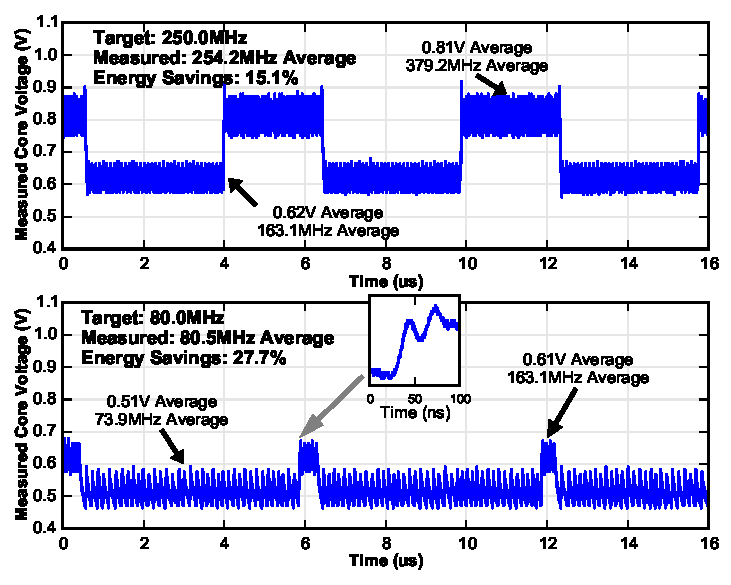
\includegraphics[width=0.8\textwidth]{6-raven4-freqhopping}
  \caption{Oscilloscope traces showing the core voltage as the frequency hopping algorithm is applied with two different frequency targets~\cite{Keller2016} ({\textcopyright} 2016 IEEE, reprinted with permission).}
  \label{fig:6-raven4-freqhopping}
\end{figure}

The programmable PMU allows the implementation of a wide variety of power management algorithms to improve energy efficiency.
Several different experiments demonstrate the flexibility of the system in implementing common energy-saving techniques.
In one experiment, dithering between two voltages to achieve an arbitrary target core frequency is implemented.
To implement this algorithm, the PMU first calibrates the system by using the core clock counter to measure the average operating frequency at each voltage mode.
Then a target frequency is provided to the PMU, which polls the core clock counter and dithers the voltage setting to achieve the target frequency in aggregate.
The results of the experiment are shown in Figure~\ref{fig:6-raven4-freqhopping}.
Without dithering, the processor would need to operate only in the higher mode to guarantee that the performance target is met, which would consume up to 40\% more energy than the dithered approach.

The choice of hopping frequency presents a tradeoff between increased fidelity to the target effective frequency and the more frequent occurrence of transition overheads, which can increase energy consumption.
In the testchip SS-SC implementation, the energy cost associated with transitions between voltage modes is small because the processor continues to operate as the clock frequency adjusts during the mode transition.
In high-to-low mode transitions, no charge is wasted, but in some low-to-high transitions, the flying capacitance is charged to \SI{1}{\volt}, consuming wasted energy:
\begin{equation}
E_{loss}=\frac{1}{2}C_{fly}\Delta V^2
\end{equation}
In the worst-case transition from \SI{1}{\volt} 2/3 mode to \SI{1.8}{\volt} 1/2 mode, the flying capacitance is charged from roughly \SI{0.33}{\volt}, resulting in an $E_{loss}$ of roughly \SI{1}{\nano\joule}.
At a typical core operating power of \SI{50}{\milli\watt}, this loss is equivalent to the energy consumed by just \SI{20}{\nano\second} of normal operation.
Accordingly, a hopping frequency of approximately \SI{6}{\micro\second} was chosen.
This frequency is still quite fast, but is slow enough that transition energy costs can be neglected.

\begin{figure}
  \centering
  %\hspace*{\fill}
  \begin{subfigure}[t]{0.8\textwidth}
  \centering
  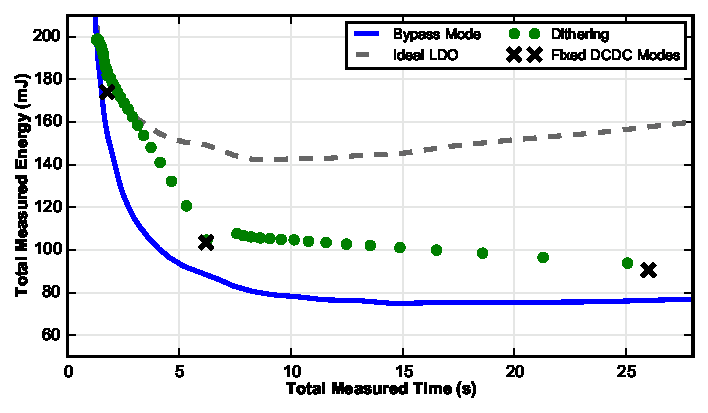
\includegraphics[width=\textwidth]{6-raven4-voltage-dithering-a}
  \caption{}
  \label{fig:6-raven4-voltage-dithering-a}
  \end{subfigure}
  %\hspace*{\fill}
  \par\bigskip
  \begin{subfigure}[t]{0.8\textwidth}
  \centering
  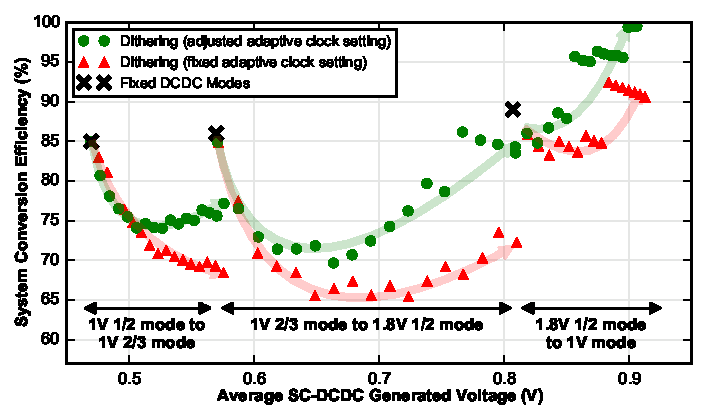
\includegraphics[width=\textwidth]{6-raven4-voltage-dithering-b}
  \caption{}
  \label{fig:6-raven4-voltage-dithering-b}
  \end{subfigure}
  %\hspace*{\fill}
  \caption{Plots showing the effect of voltage dithering on system conversion efficiency~\cite{Keller2017} ({\textcopyright} 2017 IEEE, reprinted with permission).  (\subref{fig:6-raven4-voltage-dithering-a}) compares the energy cost of dithering to the bypass mode baseline (in blue), which represents 100\% efficient regulation.  The dithering operating points linearly interpolate completion time and energy between the fixed SS-SC modes.  (\subref{fig:6-raven4-voltage-dithering-b}) shows the measured system conversion efficiencies under voltage dithering.  The results in green show the benefit of re-tuning the replica timing circuit in the adaptive clock generator after each SS-SC mode transition.}
  \label{fig:6-raven4-voltage-dithering}
\end{figure}

Voltage dithering can suffer reduced conversion efficiency compared to continuous regulation.
This effect is explored in Figure~\ref{fig:6-raven4-voltage-dithering}.
Each measured point in the figures represents the completion of a fixed-length matrix-multiply benchmark.
The dithering algorithm enables a wide operating range for the core, bounded only by the lowest and highest voltage settings of the SS-SC converter. 
Figure~\ref{fig:6-raven4-voltage-dithering-a} shows measurement results of system conversion efficiency, similar to the measured results of Raven-3 as shown in Figure~\ref{fig:6-raven3-dcdc-efficiency}.
Instead of just three conversion points, however, the interpolated time-energy points measured from dithering between each of the neighboring voltages at a fixed ratio are also shown.
Figure~\ref{fig:6-raven4-voltage-dithering-b} quantifies the effects of dithering on system conversion efficiency.
Two different dithering programs were run on the PMU.
The first program simply switches the voltage mode setting of the SS-SC converters, without changing any other system settings; the delay settings of the replica paths in the adaptive clock generator were tuned to the best setting that could function across both operating modes.
The results are shown by the red points in the figure.
Because the best setting of the replica paths changes according to operating mode, the conversion efficiencies of this approach are less than optimal for part of the dithering range.
The second program switches both the voltage mode and the delay settings of the replica paths according to a pre-characterization of the best adaptive clock setting associated with each voltage mode.
This program is able to speed the generated clock at the higher voltage settings, leading to higher conversion efficiencies.
In all, the efficiencies of the second program range from 70\% to 100\%, depending on the voltage mode and dithering ratio.
Conversion efficiencies while dithering are not as high as the efficiencies of the fixed operating modes in Table~\ref{tab:raven4-efficiency} because the external voltage reference used by the comparator cannot be tuned for a particular SS-SC mode.
This implies that in some cases it is more efficient to operate at a single mode than to dither, even if the performance target is somewhat exceeded by the average operating frequency at the fixed mode.

\begin{figure}
  \centering
  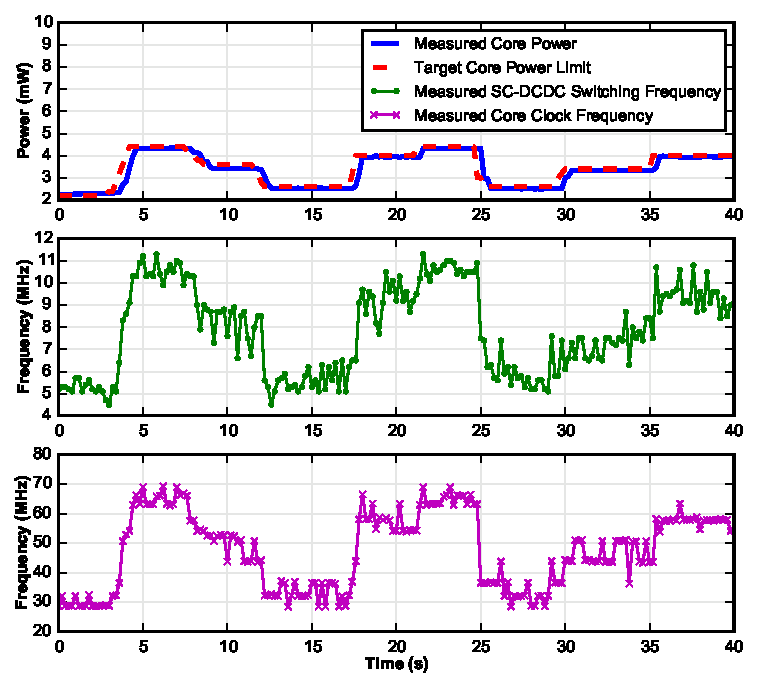
\includegraphics[width=0.8\textwidth]{6-raven4-power-tracking}
  \caption{Measurement results showing a power envelope tracking program executing on the PMU~\cite{Keller2017} ({\textcopyright} 2017 IEEE, reprinted with permission). The frequency of the core is adjusted in response to measured changes in core power so that the core operates as quickly as possible without exceeding a time-varying, user-specified power budget.}
  \label{fig:6-raven4-power-tracking}
\end{figure}

A second experiment demonstrates power envelope tracking, a common requirement for systems that must operate within a user-specified power budget.
Figure~\ref{fig:6-raven4-power-tracking} shows the results of a power management algorithm executed on the PMU that maximizes core performance within a user-specified power budget.
The power management program polls an externally writeable control register that stores the absolute power limit for the program.
The PMU core then monitors the SS-SC toggle counter to continuously estimate core power using the quadratic model described in~\cite{Cochet2016} with pre-characterized coefficients.
If the estimated core power is above the specified limit, core frequency is decreased, and if it is below the limit, core frequency is increased.
In this way, the best possible performance is automatically obtained while the user-specified power budget is respected.

\begin{figure}
  \centering
  \includegraphics[width=0.8\textwidth]{6-raven4-avs}
  \caption{Oscilloscope traces showing an FG-AVS algorithm running on the PMU~\cite{Keller2017} ({\textcopyright} 2017 IEEE, reprinted with permission).}
  \label{fig:6-raven4-avs}
\end{figure}

The PMU can also use the integrated counters to coordinate fine-grained adaptive voltage scaling (AVS) on-chip without any explicit guidance from the programs running on the processor.
In the algorithm used in this experiment, core power is used as a marker of program phase.
When core power is higher, the core is likely executing a compute-intensive program region, and a high voltage is best suited to a race-to-halt strategy. 
When the core power is lower, the core is likely waiting for off-chip communication in a memory-bound program region, and energy can be saved with minimal performance impact by reducing the voltage.
In this experiment, the application core runs a synthetic benchmark that alternates between the compute-intensive and idle phases at a timescale of tens of microseconds.
Figure~\ref{fig:6-raven4-avs} shows the core voltage measured during the execution of the benchmark and the AVS power-management algorithm.
The algorithm switches the core voltage between the \SI{1.8}{\volt} 1/2 mode and the \SI{1}{\volt} 2/3 mode, actuated by core power estimates determined by continuously polling the SS-SC toggle counter.
When the core voltage is high and the toggle rate drops below a threshold, this corresponds to an idle program period, so the PMU reduces the core voltage to save energy.
When the core voltage is low and the toggle rate exceeds a threshold, the workload has increased and the PMU increases the core voltage.
The system is able to detect changes in workload in less than \SI{1}{\micro\second} and adjust the core voltage in response.
Without integrated voltage regulators and power management, the system would not be able to respond within the timescales of the workload variation.
The results of the power-management algorithm are therefore compared against continuous operation in the higher voltage mode, which would otherwise be required to meet the same performance target.
The power-management algorithm reduces the energy consumed by 39.8\%, and the fast response incurs negligible ($<$0.2\%) performance penalty compared with this baseline because the fast response minimizes the time spent in the lower voltage mode during a compute-bound region.
This experiment demonstrates the efficacy of fine-grained AVS at improving energy efficiency with fast workload tracking.

The integrated body-bias generator achieves up to \SI{1.48}{\volt} of positive body-bias in the n-well and up to \SI{1.2}{\volt} of negative body-bias in the p-well.
The n-well voltage achieves \SI{58}{\milli\volt} resolution and the p-well voltage achieves \SI{72}{\milli\volt} resolution, corresponding in each case to roughly \SI{5}{\milli\volt} of threshold voltage step.
Figure~\ref{fig:bbgen-results-transient} shows the dynamics of charging and discharging of the wells.
The n-well reaches high slew rates of \SI{-80}{\milli\volt\per\nano\second} and \SI[retain-explicit-plus]{+65}{\milli\volt\per\nano\second} during charging and discharging.
The p-well voltage ramps down from \SI{0}{\volt} to \SI{-1.3}{\volt} in \SI{160}{\nano\second} with one driver unit, and in \SI{90}{\nano\second} with two units, switching at \SI{1}{\giga\hertz} in both cases.
The p-well discharges from \SI{1.4}{\volt} to \SI{0}{\volt} in \SI{70}{\nano\second} with only one unit operating.
During the ON-mode the BBG drives currents in the range of \SIrange[range-phrase = --]{40}{200}{\milli\ampere}, while in STEADY-mode it sources only \SI{3.3}{\micro\ampere} and \SI{1}{\micro\ampere} from the \SI{1.8}{\volt} and \SI{1}{\volt} supplies respectively.
High ON-mode currents are averaged over long periods of STEADY-mode and contribute less than \SI{2}{\micro\ampere} in total average current.
Figure~\ref{fig:bbgen-results-tracking} illustrates the maintenance of target n-well and p-well voltages with short recharge phases when the well voltages drift due to leakage.
In this case, ON-mode recharge of \SI{5}{\nano\second} duration occurs every \SI{1}{\milli\second} and \SI{0.2}{\milli\second} for the n-well and p-well respectively.
Figure~\ref{fig:bbgen-results-compensation} demonstrates the variation-compensation and energy-efficiency optimization capability of the BBG.
The frequency counters are used to extract the switching frequency of the integrated clock generator.
This frequency is influenced both by the core supply voltage and the body-bias effect.
A feedback loop adjusts the body-bias voltage so that a constant frequency is maintained even as supply voltage changes.
The design is able to maintain the target frequency within 1\% while dynamically changing the digital supply voltage in the range of \SIrange[range-phrase = --]{760}{970}{\milli\volt}.
Note that the p-well and n-well voltages can be asymmetric to achieve robust compensation.

\begin{figure}
  \centering
  %\hspace*{\fill}
  \begin{subfigure}[t]{0.8\textwidth}
  \centering
  \includegraphics[width=\textwidth]{bbgen-results-transient-a}
  \caption{}
  \label{fig:bbgen-results-transient-a}
  \end{subfigure}
  %\hspace*{\fill}
  \par\bigskip
  \begin{subfigure}[t]{0.8\textwidth}
  \centering
  \includegraphics[width=\textwidth]{bbgen-results-transient-b}
  \caption{}
  \label{fig:bbgen-results-transient-b}
  \end{subfigure}
  %\hspace*{\fill}
  \caption{Transient measurements of well charging and discharging of the p-well (\subref{fig:bbgen-results-transient-a}) and n-well (\subref{fig:bbgen-results-transient-b}) voltages~\cite{Blagojevic2016} ({\textcopyright} 2016 IEEE, reprinted with permission).}
  \label{fig:bbgen-results-transient}
\end{figure}

\begin{figure}
  \centering
  \includegraphics[width=0.8\textwidth]{bbgen-results-tracking}
  \caption{Maintaining a constant body bias with occasional recharge to compensate for leakage~\cite{Blagojevic2016} ({\textcopyright} 2016 IEEE, reprinted with permission).}
  \label{fig:bbgen-results-tracking}
\end{figure}

\begin{figure}
  \centering
  \includegraphics[width=0.8\textwidth]{bbgen-results-compensation}
  \caption{Adaptive body bias compensation to supply voltage drift~\cite{Blagojevic2016} ({\textcopyright} 2016 IEEE, reprinted with permission).  A constant frequency is maintained by adjusting body bias as supply voltage changes.}
  \label{fig:bbgen-results-compensation}
\end{figure}

\begin{acknowledgement}
The authors would like to gratefully acknowledge Ben Keller, Brian Zimmer, Martin Cochet, Yunsup Lee, Jaehwa Kwak, Alberto Puggelli, Milovan Blagojevi\'{c}, Ruzica Jevti\'{c}, Pi-Feng Chiu, Stevo Bailey, Palmer Dabbelt, Colin Schmidt, Hanh-Phuc Le, Po-Hung Chen, Nicholas Sutardja, Rimas Avizienis, Andrew Waterman, James Dunn, Brian Richards, Philippe Flatresse, Andrei Vladimirescu, Andreia Cathelin, Elad Alon, and Krste Asanovi\'{c}, who contributed substantially to the research presented in this chapter.
Fabrication of the Raven-3 and Raven-4 testchips was donated by STMicroelectronics.
The research presented in this chapter was supported by the Berkeley Wireless Research Center, the Berkeley ASPIRE Lab, DARPA PERFECT Award Number HR0011-12-2-0016, Intel ARO, AMD, SRC/TxACE, Marie Curie FP7, the NSF GRFP, and the NVIDIA Fellowship.
\end{acknowledgement}

%%%%%%%%%%%%%%%%%%%%%%%% referenc.tex %%%%%%%%%%%%%%%%%%%%%
% sample references
% 
% Use this file as a template for your own input.
%
%%%%%%%%%%%%%%%%%%%%%%%% Springer%%%%%%%%%%%%%%%%%%%%%%%%%%
%
% BibTeX users please use
% \bibliographystyle{}
% \bibliography{}
%
\biblstarthook{References may be \textit{cited} in the text either by number (preferred) or by author/year.\footnote{Make sure that all references from the list are cited in the text. Those not cited should be moved to a separate \textit{Further Reading} section or chapter.} The reference list should ideally be \textit{sorted} in alphabetical order -- even if reference numbers are used for the their citation in the text. If there are several works by the same author, the following order should be used: 
\begin{enumerate}
\item all works by the author alone, ordered chronologically by year of publication
\item all works by the author with a coauthor, ordered alphabetically by coauthor
\item all works by the author with several coauthors, ordered chronologically by year of publication.
\end{enumerate}
The \textit{styling} of references\footnote{Always use the standard abbreviation of a journal's name according to the ISSN \textit{List of Title Word Abbreviations}, see \url{http://www.issn.org/en/node/344}} depends on the subject of your book:
\begin{itemize}
\item The \textit{two} recommended styles for references in books on \textit{mathematical, physical, statistical and computer sciences} are depicted in ~\cite{science-contrib, science-online, science-mono, science-journal, science-DOI} and ~\cite{phys-online, phys-mono, phys-journal, phys-DOI, phys-contrib}.
\item Examples of the most commonly used reference style in books on \textit{Psychology, Social Sciences} are~\cite{psysoc-mono, psysoc-online,psysoc-journal, psysoc-contrib, psysoc-DOI}.
\item Examples for references in books on \textit{Humanities, Linguistics, Philosophy} are~\cite{humlinphil-journal, humlinphil-contrib, humlinphil-mono, humlinphil-online, humlinphil-DOI}.
\item Examples of the basic Springer style used in publications on a wide range of subjects such as \textit{Computer Science, Economics, Engineering, Geosciences, Life Sciences, Medicine, Biomedicine} are ~\cite{basic-contrib, basic-online, basic-journal, basic-DOI, basic-mono}. 
\end{itemize}
}

\begin{thebibliography}{99.}%
% and use \bibitem to create references.
%
% Use the following syntax and markup for your references if 
% the subject of your book is from the field 
% "Mathematics, Physics, Statistics, Computer Science"
%
% Contribution 
\bibitem{science-contrib} Broy, M.: Software engineering --- from auxiliary to key technologies. In: Broy, M., Dener, E. (eds.) Software Pioneers, pp. 10-13. Springer, Heidelberg (2002)
%
% Online Document
\bibitem{science-online} Dod, J.: Effective substances. In: The Dictionary of Substances and Their Effects. Royal Society of Chemistry (1999) Available via DIALOG. \\
\url{http://www.rsc.org/dose/title of subordinate document. Cited 15 Jan 1999}
%
% Monograph
\bibitem{science-mono} Geddes, K.O., Czapor, S.R., Labahn, G.: Algorithms for Computer Algebra. Kluwer, Boston (1992) 
%
% Journal article
\bibitem{science-journal} Hamburger, C.: Quasimonotonicity, regularity and duality for nonlinear systems of partial differential equations. Ann. Mat. Pura. Appl. \textbf{169}, 321--354 (1995)
%
% Journal article by DOI
\bibitem{science-DOI} Slifka, M.K., Whitton, J.L.: Clinical implications of dysregulated cytokine production. J. Mol. Med. (2000) doi: 10.1007/s001090000086 
%
\bigskip

% Use the following (APS) syntax and markup for your references if 
% the subject of your book is from the field 
% "Mathematics, Physics, Statistics, Computer Science"
%
% Online Document
\bibitem{phys-online} J. Dod, in \textit{The Dictionary of Substances and Their Effects}, Royal Society of Chemistry. (Available via DIALOG, 1999), 
\url{http://www.rsc.org/dose/title of subordinate document. Cited 15 Jan 1999}
%
% Monograph
\bibitem{phys-mono} H. Ibach, H. L\"uth, \textit{Solid-State Physics}, 2nd edn. (Springer, New York, 1996), pp. 45-56 
%
% Journal article
\bibitem{phys-journal} S. Preuss, A. Demchuk Jr., M. Stuke, Appl. Phys. A \textbf{61}
%
% Journal article by DOI
\bibitem{phys-DOI} M.K. Slifka, J.L. Whitton, J. Mol. Med., doi: 10.1007/s001090000086
%
% Contribution 
\bibitem{phys-contrib} S.E. Smith, in \textit{Neuromuscular Junction}, ed. by E. Zaimis. Handbook of Experimental Pharmacology, vol 42 (Springer, Heidelberg, 1976), p. 593
%
\bigskip
%
% Use the following syntax and markup for your references if 
% the subject of your book is from the field 
% "Psychology, Social Sciences"
%
%
% Monograph
\bibitem{psysoc-mono} Calfee, R.~C., \& Valencia, R.~R. (1991). \textit{APA guide to preparing manuscripts for journal publication.} Washington, DC: American Psychological Association.
%
% Online Document
\bibitem{psysoc-online} Dod, J. (1999). Effective substances. In: The dictionary of substances and their effects. Royal Society of Chemistry. Available via DIALOG. \\
\url{http://www.rsc.org/dose/Effective substances.} Cited 15 Jan 1999.
%
% Journal article
\bibitem{psysoc-journal} Harris, M., Karper, E., Stacks, G., Hoffman, D., DeNiro, R., Cruz, P., et al. (2001). Writing labs and the Hollywood connection. \textit{J Film} Writing, 44(3), 213--245.
%
% Contribution 
\bibitem{psysoc-contrib} O'Neil, J.~M., \& Egan, J. (1992). Men's and women's gender role journeys: Metaphor for healing, transition, and transformation. In B.~R. Wainrig (Ed.), \textit{Gender issues across the life cycle} (pp. 107--123). New York: Springer.
%
% Journal article by DOI
\bibitem{psysoc-DOI}Kreger, M., Brindis, C.D., Manuel, D.M., Sassoubre, L. (2007). Lessons learned in systems change initiatives: benchmarks and indicators. \textit{American Journal of Community Psychology}, doi: 10.1007/s10464-007-9108-14.
%
%
% Use the following syntax and markup for your references if 
% the subject of your book is from the field 
% "Humanities, Linguistics, Philosophy"
%
\bigskip
%
% Journal article
\bibitem{humlinphil-journal} Alber John, Daniel C. O'Connell, and Sabine Kowal. 2002. Personal perspective in TV interviews. \textit{Pragmatics} 12:257--271
%
% Contribution 
\bibitem{humlinphil-contrib} Cameron, Deborah. 1997. Theoretical debates in feminist linguistics: Questions of sex and gender. In \textit{Gender and discourse}, ed. Ruth Wodak, 99--119. London: Sage Publications.
%
% Monograph
\bibitem{humlinphil-mono} Cameron, Deborah. 1985. \textit{Feminism and linguistic theory.} New York: St. Martin's Press.
%
% Online Document
\bibitem{humlinphil-online} Dod, Jake. 1999. Effective substances. In: The dictionary of substances and their effects. Royal Society of Chemistry. Available via DIALOG. \\
http://www.rsc.org/dose/title of subordinate document. Cited 15 Jan 1999
%
% Journal article by DOI
\bibitem{humlinphil-DOI} Suleiman, Camelia, Daniel C. O�Connell, and Sabine Kowal. 2002. `If you and I, if we, in this later day, lose that sacred fire...�': Perspective in political interviews. \textit{Journal of Psycholinguistic Research}. doi: 10.1023/A:1015592129296.
%
%
%
\bigskip
%
%
% Use the following syntax and markup for your references if 
% the subject of your book is from the field 
% "Computer Science, Economics, Engineering, Geosciences, Life Sciences"
%
%
% Contribution 
\bibitem{basic-contrib} Brown B, Aaron M (2001) The politics of nature. In: Smith J (ed) The rise of modern genomics, 3rd edn. Wiley, New York 
%
% Online Document
\bibitem{basic-online} Dod J (1999) Effective Substances. In: The dictionary of substances and their effects. Royal Society of Chemistry. Available via DIALOG. \\
\url{http://www.rsc.org/dose/title of subordinate document. Cited 15 Jan 1999}
%
% Journal article by DOI
\bibitem{basic-DOI} Slifka MK, Whitton JL (2000) Clinical implications of dysregulated cytokine production. J Mol Med, doi: 10.1007/s001090000086
%
% Journal article
\bibitem{basic-journal} Smith J, Jones M Jr, Houghton L et al (1999) Future of health insurance. N Engl J Med 965:325--329
%
% Monograph
\bibitem{basic-mono} South J, Blass B (2001) The future of modern genomics. Blackwell, London 
%
\end{thebibliography}


\printbibliography

\end{document}





% Original Springer template is below


%\section{Section Heading}
%\label{sec:1}
%Use the template \emph{chapter.tex} together with the Springer document class SVMono (monograph-type books) or SVMult (edited books) to style the various elements of your chapter content in the Springer layout.
%
%Instead of simply listing headings of different levels we recommend to let every heading be followed by at least a short passage of text. Further on please use the \LaTeX\ automatism for all your cross-references and citations. And please note that the first line of text that follows a heading is not indented, whereas the first lines of all subsequent paragraphs are.
%
%\section{Section Heading}
%\label{sec:2}
%% Always give a unique label
%% and use \ref{<label>} for cross-references
%% and \cite{<label>} for bibliographic references
%% use \sectionmark{}
%% to alter or adjust the section heading in the running head
%Instead of simply listing headings of different levels we recommend to let every heading be followed by at least a short passage of text. Further on please use the \LaTeX\ automatism for all your cross-references and citations.
%
%Please note that the first line of text that follows a heading is not indented, whereas the first lines of all subsequent paragraphs are.
%
%Use the standard \verb|equation| environment to typeset your equations, e.g.
%%
%\begin{equation}
%a \times b = c\;,
%\end{equation}
%%
%however, for multiline equations we recommend to use the \verb|eqnarray|
%environment\footnote{In physics texts please activate the class option
%\texttt{vecphys} to depict your vectors in \textbf{\itshape
%boldface-italic} type - as is customary for a wide range of physical
%subjects}.
%\begin{eqnarray}
%a \times b = c \nonumber\\
%\vec{a} \cdot \vec{b}=\vec{c}
%\label{eq:01}
%\end{eqnarray}
%
%\subsection{Subsection Heading}
%\label{subsec:2}
%Instead of simply listing headings of different levels we recommend to let every heading be followed by at least a short passage of text. Further on please use the \LaTeX\ automatism for all your cross-references\index{cross-references} and citations\index{citations} as has already been described in Sect.~\ref{sec:2}.
%
%\begin{quotation}
%Please do not use quotation marks when quoting texts! Simply use the \verb|quotation| environment -- it will automatically render Springer's preferred layout.
%\end{quotation}
%
%
%\subsubsection{Subsubsection Heading}
%Instead of simply listing headings of different levels we recommend to let every heading be followed by at least a short passage of text. Further on please use the \LaTeX\ automatism for all your cross-references and citations as has already been described in Sect.~\ref{subsec:2}, see also Fig.~\ref{fig:1}\footnote{If you copy text passages, figures, or tables from other works, you must obtain \textit{permission} from the copyright holder (usually the original publisher). Please enclose the signed permission with the manuscript. The sources\index{permission to print} must be acknowledged either in the captions, as footnotes or in a separate section of the book.}
%
%Please note that the first line of text that follows a heading is not indented, whereas the first lines of all subsequent paragraphs are.
%
%% For figures use
%%
%\begin{figure}[b]
%\sidecaption
%% Use the relevant command for your figure-insertion program
%% to insert the figure file.
%% For example, with the graphicx style use
%\includegraphics[scale=.65]{figure}
%%
%% If no graphics program available, insert a blank space i.e. use
%%\picplace{5cm}{2cm} % Give the correct figure height and width in cm
%%
%\caption{If the width of the figure is less than 7.8 cm use the \texttt{sidecapion} command to flush the caption on the left side of the page. If the figure is positioned at the top of the page, align the sidecaption with the top of the figure -- to achieve this you simply need to use the optional argument \texttt{[t]} with the \texttt{sidecaption} command}
%\label{fig:1}       % Give a unique label
%\end{figure}
%
%
%\paragraph{Paragraph Heading} %
%Instead of simply listing headings of different levels we recommend to let every heading be followed by at least a short passage of text. Further on please use the \LaTeX\ automatism for all your cross-references and citations as has already been described in Sect.~\ref{sec:2}.
%
%Please note that the first line of text that follows a heading is not indented, whereas the first lines of all subsequent paragraphs are.
%
%For typesetting numbered lists we recommend to use the \verb|enumerate| environment -- it will automatically render Springer's preferred layout.
%
%\begin{enumerate}
%\item{Livelihood and survival mobility are oftentimes coutcomes of uneven socioeconomic development.}
%\begin{enumerate}
%\item{Livelihood and survival mobility are oftentimes coutcomes of uneven socioeconomic development.}
%\item{Livelihood and survival mobility are oftentimes coutcomes of uneven socioeconomic development.}
%\end{enumerate}
%\item{Livelihood and survival mobility are oftentimes coutcomes of uneven socioeconomic development.}
%\end{enumerate}
%
%
%\subparagraph{Subparagraph Heading} In order to avoid simply listing headings of different levels we recommend to let every heading be followed by at least a short passage of text. Use the \LaTeX\ automatism for all your cross-references and citations as has already been described in Sect.~\ref{sec:2}, see also Fig.~\ref{fig:2}.
%
%For unnumbered list we recommend to use the \verb|itemize| environment -- it will automatically render Springer's preferred layout.
%
%\begin{itemize}
%\item{Livelihood and survival mobility are oftentimes coutcomes of uneven socioeconomic development, cf. Table~\ref{tab:1}.}
%\begin{itemize}
%\item{Livelihood and survival mobility are oftentimes coutcomes of uneven socioeconomic development.}
%\item{Livelihood and survival mobility are oftentimes coutcomes of uneven socioeconomic development.}
%\end{itemize}
%\item{Livelihood and survival mobility are oftentimes coutcomes of uneven socioeconomic development.}
%\end{itemize}
%
%\begin{figure}[t]
%\sidecaption[t]
%% Use the relevant command for your figure-insertion program
%% to insert the figure file.
%% For example, with the option graphics use
%\includegraphics[scale=.65]{figure}
%%
%% If no graphics program available, insert a blank space i.e. use
%%\picplace{5cm}{2cm} % Give the correct figure height and width in cm
%%
%%\caption{Please write your figure caption here}
%\caption{If the width of the figure is less than 7.8 cm use the \texttt{sidecapion} command to flush the caption on the left side of the page. If the figure is positioned at the top of the page, align the sidecaption with the top of the figure -- to achieve this you simply need to use the optional argument \texttt{[t]} with the \texttt{sidecaption} command}
%\label{fig:2}       % Give a unique label
%\end{figure}
%
%\runinhead{Run-in Heading Boldface Version} Use the \LaTeX\ automatism for all your cross-references and citations as has already been described in Sect.~\ref{sec:2}.
%
%\subruninhead{Run-in Heading Italic Version} Use the \LaTeX\ automatism for all your cross-refer\-ences and citations as has already been described in Sect.~\ref{sec:2}\index{paragraph}.
%% Use the \index{} command to code your index words
%%
%% For tables use
%%
%\begin{table}
%\caption{Please write your table caption here}
%\label{tab:1}       % Give a unique label
%%
%% Follow this input for your own table layout
%%
%\begin{tabular}{p{2cm}p{2.4cm}p{2cm}p{4.9cm}}
%\hline\noalign{\smallskip}
%Classes & Subclass & Length & Action Mechanism  \\
%\noalign{\smallskip}\svhline\noalign{\smallskip}
%Translation & mRNA$^a$  & 22 (19--25) & Translation repression, mRNA cleavage\\
%Translation & mRNA cleavage & 21 & mRNA cleavage\\
%Translation & mRNA  & 21--22 & mRNA cleavage\\
%Translation & mRNA  & 24--26 & Histone and DNA Modification\\
%\noalign{\smallskip}\hline\noalign{\smallskip}
%\end{tabular}
%$^a$ Table foot note (with superscript)
%\end{table}
%%
%\section{Section Heading}
%\label{sec:3}
%% Always give a unique label
%% and use \ref{<label>} for cross-references
%% and \cite{<label>} for bibliographic references
%% use \sectionmark{}
%% to alter or adjust the section heading in the running head
%Instead of simply listing headings of different levels we recommend to let every heading be followed by at least a short passage of text. Further on please use the \LaTeX\ automatism for all your cross-references and citations as has already been described in Sect.~\ref{sec:2}.
%
%Please note that the first line of text that follows a heading is not indented, whereas the first lines of all subsequent paragraphs are.
%
%If you want to list definitions or the like we recommend to use the Springer-enhanced \verb|description| environment -- it will automatically render Springer's preferred layout.
%
%\begin{description}[Type 1]
%\item[Type 1]{That addresses central themes pertainng to migration, health, and disease. In Sect.~\ref{sec:1}, Wilson discusses the role of human migration in infectious disease distributions and patterns.}
%\item[Type 2]{That addresses central themes pertainng to migration, health, and disease. In Sect.~\ref{subsec:2}, Wilson discusses the role of human migration in infectious disease distributions and patterns.}
%\end{description}
%
%\subsection{Subsection Heading} %
%In order to avoid simply listing headings of different levels we recommend to let every heading be followed by at least a short passage of text. Use the \LaTeX\ automatism for all your cross-references and citations citations as has already been described in Sect.~\ref{sec:2}.
%
%Please note that the first line of text that follows a heading is not indented, whereas the first lines of all subsequent paragraphs are.
%
%\begin{svgraybox}
%If you want to emphasize complete paragraphs of texts we recommend to use the newly defined Springer class option \verb|graybox| and the newly defined environment \verb|svgraybox|. This will produce a 15 percent screened box 'behind' your text.
%
%If you want to emphasize complete paragraphs of texts we recommend to use the newly defined Springer class option and environment \verb|svgraybox|. This will produce a 15 percent screened box 'behind' your text.
%\end{svgraybox}
%
%
%\subsubsection{Subsubsection Heading}
%Instead of simply listing headings of different levels we recommend to let every heading be followed by at least a short passage of text. Further on please use the \LaTeX\ automatism for all your cross-references and citations as has already been described in Sect.~\ref{sec:2}.
%
%Please note that the first line of text that follows a heading is not indented, whereas the first lines of all subsequent paragraphs are.
%
%\begin{theorem}
%Theorem text goes here.
%\end{theorem}
%%
%% or
%%
%\begin{definition}
%Definition text goes here.
%\end{definition}
%
%\begin{proof}
%%\smartqed
%Proof text goes here.
%\qed
%\end{proof}
%
%\paragraph{Paragraph Heading} %
%Instead of simply listing headings of different levels we recommend to let every heading be followed by at least a short passage of text. Further on please use the \LaTeX\ automatism for all your cross-references and citations as has already been described in Sect.~\ref{sec:2}.
%
%Note that the first line of text that follows a heading is not indented, whereas the first lines of all subsequent paragraphs are.
%%
%% For built-in environments use
%%
%\begin{theorem}
%Theorem text goes here.
%\end{theorem}
%%
%\begin{definition}
%Definition text goes here.
%\end{definition}
%%
%\begin{proof}
%\smartqed
%Proof text goes here.
%\qed
%\end{proof}
%

%
%\section*{Appendix}
%\addcontentsline{toc}{section}{Appendix}
%%
%%
%When placed at the end of a chapter or contribution (as opposed to at the end of the book), the numbering of tables, figures, and equations in the appendix section continues on from that in the main text. Hence please \textit{do not} use the \verb|appendix| command when writing an appendix at the end of your chapter or contribution. If there is only one the appendix is designated ``Appendix'', or ``Appendix 1'', or ``Appendix 2'', etc. if there is more than one.
%
%\begin{equation}
%a \times b = c
%\end{equation}

